%% Copernicus Publications Manuscript Preparation Template for LaTeX Submissions
%% ---------------------------------
%% This template should be used for copernicus.cls
%% The class file and some style files are bundled in the Copernicus Latex Package, which can be downloaded from the different journal webpages.
%% For further assistance please contact Copernicus Publications at: production@copernicus.org
%% https://publications.copernicus.org/for_authors/manuscript_preparation.html


%% Please use the following documentclass and journal abbreviations for preprints and final revised papers.

%%2-column papers and preprints
\documentclass[journal abbreviation, manuscript]{copernicus}



%% Journal abbreviations (please use the same for preprints and final revised papers)


% Advances in Geosciences (adgeo)
% Advances in Radio Science (ars)
% Advances in Science and Research (asr)
% Advances in Statistical Climatology, Meteorology and Oceanography (ascmo)
% Annales Geophysicae (angeo)
% Archives Animal Breeding (aab)
% ASTRA Proceedings (ap)
% Atmospheric Chemistry and Physics (acp)
% Atmospheric Measurement Techniques (amt)
% Biogeosciences (bg)
% Climate of the Past (cp)
% DEUQUA Special Publications (deuquasp)
% Drinking Water Engineering and Science (dwes)
% Earth Surface Dynamics (esurf)
% Earth System Dynamics (esd)
% Earth System Science Data (essd)
% E&G Quaternary Science Journal (egqsj)
% European Journal of Mineralogy (ejm)
% Fossil Record (fr)
% Geochronology (gchron)
% Geographica Helvetica (gh)
% Geoscience Communication (gc)
% Geoscientific Instrumentation, Methods and Data Systems (gi)
% Geoscientific Model Development (gmd)
% History of Geo- and Space Sciences (hgss)
% Hydrology and Earth System Sciences (hess)
% Journal of Bone and Joint Infection (jbji)
% Journal of Micropalaeontology (jm)
% Journal of Sensors and Sensor Systems (jsss)
% Magnetic Resonance (mr)
% Mechanical Sciences (ms)
% Natural Hazards and Earth System Sciences (nhess)
% Nonlinear Processes in Geophysics (npg)
% Ocean Science (os)
% Primate Biology (pb)
% Proceedings of the International Association of Hydrological Sciences (piahs)
% Scientific Drilling (sd)
% SOIL (soil)
% Solid Earth (se)
% The Cryosphere (tc)
% Weather and Climate Dynamics (wcd)
% Web Ecology (we)
% Wind Energy Science (wes)


%% \usepackage commands included in the copernicus.cls:
%\usepackage[german, english]{babel}
%\usepackage{tabularx}
%\usepackage{cancel}
%\usepackage{multirow}
%\usepackage{supertabular}
%\usepackage{algorithmic}
%\usepackage{algorithm}
%\usepackage{amsthm}
%\usepackage{float}
%\usepackage{subfig}
%\usepackage{rotating}



\begin{document}


\title{DisReserv (v1.0): Analytical displacement solution due to reservoir compaction with arbitrary geometry and under arbitrary pressure changes}


% \Author[affil]{given_name}{surname}

\Author[1]{Valeria}{C. F. Barbosa}
\Author[1]{Vanderlei}{C. Oliveira Jr.}
\Author[1,2]{Andre}{D. Arelaro}

\affil[1]{Department of Geophysics, Observat\'{o}rio Nacional, Rio de Janeiro, Brazil}
\affil[2]{PETROBRAS, Rio de Janeiro, Brazil}


%% The [] brackets identify the author with the corresponding affiliation. 1, 2, 3, etc. should be inserted.

%% If an author is deceased, please mark the respective author name(s) with a dagger, e.g. "\Author[2,$\dag$]{Anton}{Aman}", and add a further "\affil[$\dag$]{deceased, 1 July 2019}".

%% If authors contributed equally, please mark the respective author names with an asterisk, e.g. "\Author[2,*]{Anton}{Aman}" and "\Author[3,*]{Bradley}{Bman}" and add a further affiliation: "\affil[*]{These authors contributed equally to this work.}".


\correspondence{Valeria C. F. Barbosa (valcris@on.br)}

\runningtitle{Displacement due to reservoir compaction}

\runningauthor{Barbosa, V. C. F., Oliveira Jr., V. C. and Arelaro, A. D.}



\received{}
\pubdiscuss{} %% only important for two-stage journals
\revised{}
\accepted{}
\published{}

%% These dates will be inserted by Copernicus Publications during the typesetting process.


\firstpage{1}

\maketitle


%%\twocolumn
\begin{abstract}
We have presented analytical solutions for the displacement due to reservoir compaction with arbitrary geometry and under arbitrary pressure changes.
These solutions are based on the similarity between the gravitational potential yielded 
by a volume source under a density variation and the thermoelastic displacement 
potential yielded by a volume source in a half-space under a pressure variation.
This similarity enables the use of closed expressions of the gravitational potential 
and its derivatives for calculating the displacement and stress fields due to a volume 
source under a pressure variation.
We discretized the reservoir as a grid of 3D right rectangular prisms  juxtaposed in 
the horizontal and vertical directions.
Each prism has homogeneous pressure; however, pressure variations among different 
prisms are allowed. 
This parametrization of the reservoir yields a piecewise-constant distribution of 
pressure in the subsurface. 
The discrete reservoir modeling to calculate the displacement and stress fields due to 
this pressure variation follows the nucleus-of-strain concept.
The nucleus of strain is considered an infinitesimal reservoir volume element.
The displacement and stress fields due each prism are calculated by integrating the 
nucleus of strain over the volume of the prism.
Finally, the displacement and stress due to the reservoir are computed by the sum of 
the contributions of each prism.
We provide a Python implementation (DisReserv) of our method to calculate the 
displacement and stress fields due to a reservoir with arbitrary shape and distribution 
of pressure changes. 
Our expressions are valid both inside and outside the reservoir. 
We calculate the displacement and stress fields in three scenarios: i) cylindrical 
reservoir under uniform depletion; ii) cylindrical reservoir under non uniform
depletion and iii) reservoir with arbitrary geometry and under arbitrary pressure 
distribution.
The results obtained for the three scenarios show that our method produces null 
stress field components at the free surface.
\end{abstract}


\copyrightstatement{}


\introduction  %% \introduction[modified heading if necessary]
The surface subsidence due to oil or gas withdrawal from a reservoir in the subsurface may occur as a result of geomechanical changes caused by pressure drop.
The phenomenon of subsidence by fluid extraction  has been observed in a variety of oil fields, e.g., the Ekofisk field, southern North Sea \citep{Borges2020} and the Groningen gas field in the northeast Netherlands \citep{vanThienen-visser&Fokker17}.
Because the subsidence close to hydrocarbon fields under production can induce earthquakes (e.g., \citeauthor{Dahmetal15}, \citeyear{Dahmetal15}; \citeauthor{Grigolietal17}, \citeyear{Grigolietal17}), the petroleum companies  have been an increased interest in monitoring the magnitude and distribution of subsidence resulting from reservoir depletion.
The subsidence monitoring is accomplished by means of calculating the displacement field for a given set of  reservoir properties.

The possibility of occurrence of catastrophic events, related to subsidence due to extraction or injection of fluids in reservoir, has stimulated efforts to  develop analytical methods for modeling the displacement and stress fields due to reservoir compactation.
The physical foundation of the displacement, stress and strain fields in the subsurface due to a reduction of pressure in the reservoir comes from the theory of thermoelasticity.
Theory of thermoelasticity has been laid in the first half of the nineteenth century to describe the interaction between the thermal field and elastic bodies.
In the uncoupled thermoelasticity theory for quasi-static problems (i.e., problems with negligible inertia effects), \cite{Goodier37} employed the method of superposition using
displacement potential functions and introduced the  concept of nucleus of thermoelastic strain in an infinite space.
Specifically, Goodier’s (\citeyear{Goodier37}) method simplified the thermoelastic problem by replacing it by an isothermal elastic problem with different boundary conditions together with the solution of a Poisson’s equation \citep{Tao71}. 
\cite{Mindlin&Cheng50} and \cite{Sen51} extended the Goodier's method to a homogenous half-space.
\cite{Sharma56} deduced the displacement and stress fields in an infinite elastic plate due to a nucleus of thermoelastic strain located at a point inside it by using infinite integrals involving Bessel functions.

The subsidence resulting from reservoir depletion is in the context of poroelastic theory. 
\cite{Geertsma57} remarked the analogy between the theories of thermoelasticity and poroelasticity.
To our knowledge, \cite{Geertsma73} was the first to solve the poroelastic problem by using the nucleus-of-strain concept in the half-space, which in turn was proposed by \cite{Mindlin&Cheng50} and \cite{Sen51} in the theory of thermoelasticity.
\cite{Geertsma73} derived analytical expressions for the stress and displacement fields for a thin disk-shaped reservoir. 
\cite{Segall92} followed \cite{Geertsma73} and extended the analytical solutions of the displacement and stress fields assuming general axisymmetric geometries and an arbitrary radial pressure distribution. 

\cite{Geertsma&Opstal73} applied the nucleus-of-strain concept in the half-space 
to calculate the spatial subsidence distribution due to the production of reservoir with an arbitrary 3D shape.
By assuming a producing reservoir embedded in an a homogeneous, isotropic, and elastic medium, and a reservoir model in which the pressure perturbations are related to the displacement field by a linear relationship, \cite{Geertsma&Opstal73} discretized the reservoir into a grid of  prisms and calculated the displacement due to the pressure change in the whole reservoir  by the superposition of the displacement due to the constant pressure change in each prism.
\cite{Tempone10} adopted the same reservoir model used in \cite{Geertsma&Opstal73} and 
extended the nucleus-of-strain concept in the half-space to consider the effects of a rigid basement. 
Similarly, \cite{Tempone10} assumed a reservoir embedded in an a homogeneous, isotropic, and elastic medium and calculated the displacement, stress and strain fields subject to uniform depletion.
The main drawbacks in \cite{Geertsma&Opstal73} and \cite{Tempone10} are the assumption of homogeneous reservoir and the solution is only valid outside the reservoir.
In this case, the displacements within the reservoir are calculated by a linear interpolation of the displacements at the upper and lower edges of the reservoir \citep{Tempone12}.

Considering an inhomogeneous poroelastic model consists of layered stratigraphy, \cite{Mehrabian&Abousleiman15} developed closed-form formulae for the  displacement and stress  fields outside and inside of the reservoir embedded within elastic strata with different mechanical properties and subjected to pore pressure disturbances due to fluid extraction or injection. 
By assuming a linear elastic semi-infinite medium, \cite{Munoz&Roehl17} developed analytical solution for the  displacement field  outside and inside of an arbitrarily-shaped reservoir under arbitrary distribution of pressure changes. 
\cite{Munoz&Roehl17} parametrized the reservoir into a grid of 3D prisms and used the nucleus-of-strain concept. 
The nucleus of strain is taking as an infinitesimal volume element  for each prism and the displacement solution due to each prism is obtained by a three-dimensional integration over the prism volume. 
The displacement field outside and inside of the reservoir is given by the summation of the displacement fields of the displacements produced by all prisms setting up the reservoir model.
 
The present work assumes a linear elastic semi-infinite medium and provides an analytical solution for displacement field due to an arbitrarily-shaped reservoir under arbitrary distribution of pressure changes. 
Like \cite{Munoz&Roehl17} we used the nucleus-of-strain concept and discretized the
reservoir into a grid of 3D prisms along the $x-$, $y-$ and $-z$ directions.
We also consider the nucleus of strain as an infinitesimal volume element  for each prism and the displacement solution due to each prism is obtained by a three-dimensional integration over the prism volume. 
The final displacement field due to the whole reservoir is the sum of the displacements produced by the prisms. 
In contrast with \cite{Munoz&Roehl17}'s method we take advantage the similarity between 
the  equations for calculating the displacement field due to a volume source in a half-space under a pressure variation and the gravitational potential due to a volume source under a density variation.
This similarity makes possible the use of closed expressions of the gravitational potential and its derivatives produced by the 3D right rectangular prism derived by \cite{Nagyetal2000} and (\citeyear{Nagyetal2002}) and \cite{Fukushima2020}  for calculating the displacement field due to a volume source under a pressure variation.
The adopted exact analytical formulae of the gravitational field  are valid expressions either outside or inside the prisms because the implemented expressions make use of  modified arctangent function proposed by \cite{Fukushima2020}. 
We present routines written in Python language (Python 3.7.6)  to calculate the displacement fields due to a reservoir with arbitrary shape and distribution of pressure changes. 
We validate our equations by verifying that at the free surface the stress fields are null.
Tests with synthetic data validate our approach. 

\section{THEORY}

The displacement, stress and strain fields in the subsurface caused by reservoir compactation due to hydrocarbon production are grounded on the theory of thermoelasticity. 

The Goodier’s thermoelastic displacement potential $\phi$ satisfies the Poisson's equation \citep{Goodier37}, i.e.:
\begin{equation}
\nabla^{2} \phi =  m \: T,
\label{eq:poisson}
\end{equation}
where $\nabla^{2}$ is the Laplacian operator, $T $ is the temperature variation and 
\begin{equation}
m =  \:  \alpha \: \frac{1 + \nu}{ 1 -\nu},
\label{eq:m}
\end{equation}
where $\alpha$ is the coefficient of linear thermal expansion and $\nu$ is the Poisson's ratio.

From the potential theory, a particular solution of equation \ref{eq:poisson} is
\begin{equation}
\phi(x,y,z) = -  \frac{m}{4 \pi} \int\int\limits_{v}\int \frac{T(x^{\prime}, y^{\prime}, z^{\prime} )}{\sqrt{(x - x^{\prime})^{2} + (y - y^{\prime})^{2} + (z - z^{\prime})^{2}}} \: dv^{\prime},
\label{eq:phi}
\end{equation}
where $\phi(x,y,z)$ represents the Newtonian gravitational potential \citep{Kellogg29} that would be produced at the coordinates $x, y$ and $z$ by a continuous density distribution $- \frac{m}{4 \pi}  \: T( x^{\prime}, y^{\prime}, z^{\prime} )$. 
The integral in equation \ref{eq:phi} is conducted over the coordinates $x^{\prime}$,$y^{\prime}$ and $z^{\prime}$, denoting, respectively, the $x-$, $y-$ and $-z$ coordinates of an arbitrary point belonging to the interior of the volume $v$ of the solid. 


From equation \ref{eq:phi} and the potential theory, \citet{Goodier37} showed that, if an element of volume $dv$ in the infinite solid is at a temperature $T(x^{\prime}, y^{\prime}, z^{\prime}) $, the remainder being at temperature zero, the displacement vector $\bf{u}$ caused by this temperature is the gradient of the Goodier’s thermoelastic displacement potential, i.e.,
\begin{equation}
{\bf{u}} = {\bf {\nabla}} \phi(x,y,z) \: ,
\label{eq:displacement-general}
\end{equation}
where $\bf{\nabla}$ is the gradient operator.  

To a homogenous half-space, \citet{Mindlin&Cheng50} showed that the method proposed by  \citet{Goodier37} can be extended by the displacement solution given by:
\begin{equation}
\bf{u} = {\bf{\nabla}} \: \phi_{1} \: + \: {\bf{{\nabla}_{2}}} \phi_{2}, 
\label{eq:displacement-solution}
\end{equation}
where $\phi_{1} \equiv \phi_{1}(x,y,z)$ is the potential defined in equation \ref{eq:phi}, 
$\phi_{2} \equiv  \phi_{2}(x,y,z)$
is defined as "image potential" \citep{Segall92} due to a image point at the coordinates
$(x^{\prime}, y^{\prime}, -z^{\prime} )$ and the operator $\bf{{\nabla}_{2}}$ is expressed by
\begin{equation}
{\bf{{\nabla}_{2}}} = (3 - 4\nu){\bf{\nabla}} + 2 {\bf{\nabla}} z \frac{\partial }{\partial z}  - 4(1- \nu){\bf{\hat{z}}} {\bf{{\nabla}^{2}_{z}}},
\label{eq:nabla2}
\end{equation}
where ${\bf{\hat{z}}}$ is the unit vector in the $z-$direction and 
${\bf{{\nabla}^{2}_{z}}}$ is a scalar operator in which the operand is firstly
multiplied by $z$ and then operated upon by the Laplacian ${\bf{\nabla}^{2}}$. 

Equation \ref{eq:displacement-solution} is the displacement solution for the variation of temperature due to a single nucleus of strain buried at depth $z^{\prime}$ in a
semi-infinite homogeneous medium. 
In the right hand side of equation \ref{eq:displacement-solution}, the first term 
$ {\bf{\nabla}} \: \phi_{1} $ represents the displacement in an infinite medium, and the second term represents a correction of the displacement due a half-space, also known as "image nucleus solution".

\section{METHODOLOGY}

Let's assume that a reservoir in the interior of the Earth is subject to a compactation due to hydrocarbon production. 
The compactation is caused by the pressure change within the reservoir, which in turn causes  a surface subsidence (or surface displacement). 
Here, we use a Cartesian coordinate system with the $x-$axis pointing to north, the $y-$axis pointing to east and the $z-$axis pointing downward.
We discretize the reservoir into an $ m_{x} \times m_{y} \times m_{z} $ grid of 3D vertical juxtaposed prisms $(m_{x} \cdot m_{y} \cdot m_{z} = M)$ along the 
$x$, $y$ and $z$ axes, respectively, in which the pressure within each prism is 
assumed to be constant and known. 
Each prism in the reservoir model may undergo a distinct pressure change.
The subsidence effect is the displacement field due to the pressure change throughout the reservoir and is calculated by the sum of the displacement produced by each prism.


The discrete forward modeling to calculate the displacement and stress fields due to a piecewise-constant distribution of the pressure contrast within a reservoir follows the nucleus-of-strain approach. 
We assume that a nucleus of strain represents an infinitesimal reservoir volume 
element. The displacement solution for a single nucleus of strain in a homogeneous elastic semi-infinite medium (equation \ref{eq:displacement-solution}) will be used as an element of the displacement.
Then we calculate the displacement field due to the pressure contrast of a prism by integrating the nucleus of strain over its volume. The same approach is used to 
compute the stress field due to a prism.


\subsection{The discrete forward modeling due to a nucleus of strain in a homogeneous elastic semi-infinite medium}\label{solution-nucleus}

By considering the discrete form of equation \ref{eq:displacement-solution}, the displacement vector  $ {\bf{u}}_{ij} \equiv  {\bf{u}}(x_{i}, y_{i}, z_{i}, x^{\prime}_{j}, y^{\prime}_{j}, z^{\prime}_{j})$ at an arbitrary point $(x_{i}, y_{i}, z_{i})$ due to the $j$th nucleus of strain at the coordinates 
$(x^{\prime}_{j}, y^{\prime}_{j}, z^{\prime}_{j})$ will be calculated by
\begin{equation}
{\bf{u}}_{ij}  = {\bf{u_{1}}}_{ij} + {\bf{u_{2}}}_{ij} \: ,
\label{eq:displacement_ui}
\end{equation}
where ${\bf{u_{1}}}_{ij}$ is the displacement vector at the point $(x_{i}, y_{i}, z_{i})$ due to the $j$th single nucleus in the infinite space and ${\bf{u_{2}}}_{ij}$ 
is the correction of the displacement considering a semi-space (image nucleus solution).
The term ${\bf{u_{1}}}_{ij}$ (equation \ref{eq:displacement_ui}) is given by
\begin{equation}
{\bf{u_{1}}}_{ij} = \frac{A  \: (1 + \nu)}{E} \: {\bf{\nabla}} \bigg( {\frac{1}{{R_1}_{ij}}} \bigg) 
\: \Delta p_{j} \: \:dv_j^{\prime}
\label{eq:nucleus-u1}
\end{equation}
and represents the gradient of the potential
\begin{equation}
\phi_{1} = - \frac{C_m}{4 \pi}  \frac{\Delta p_{j} \: \:dv_j^{\prime}}{ {R_1}_{ij} } \: .
\label{eq:nucleus-phi1}
\end{equation}
The term ${\bf{u_{2}}}_{ij}$ (equation \ref{eq:displacement_ui}) is given by
\begin{equation}
{\bf{u_{2}}}_{ij} = \frac{A  \: (1 + \nu)}{E} \: 
\bigg[ 
(3 - 4\nu){\bf{\nabla}} \bigg(  {\frac{1}{{R_2}_{ij}}} \bigg)     
+ 2 {\bf{\nabla}} \bigg( z \frac{\partial }{\partial z} {\frac{1}{{R_2}_{ij}}} \bigg)  
- 4(1- \nu){\bf{\hat{z}}} {\bf{{\nabla}^{2}}}  \bigg( {\frac{z}{{R_2}_{ij}}} \bigg)
\bigg]   \: \Delta p_{j}  \:dv_j^{\prime}
\label{eq:nucleus-u2}
\end{equation}
and is obtained by applying the operator ${\bf{{\nabla}_{2}}}$ (equation 
\ref{eq:nabla2}) to the image potential
\begin{equation}
\phi_{2} = - \frac{C_m}{4 \pi}  \frac{\Delta p_{j} \: \:dv_j^{\prime}}{ {R_2}_{ij} } \: .
\label{eq:nucleus-phi2}
\end{equation}
In equations \ref{eq:nucleus-u1}--\ref{eq:nucleus-phi2}, 
all derivatives are computed with respect to the coordinates of the point 
$(x_{i}, y_{i}, z_{i})$, 
$\Delta p_j$  is the pressure contrast of the $j$th nucleus, $dv_j^{\prime}$ is an 
infinitesimal element of volume centered at the $j$th nucleus of strain 
$(x^{\prime}_{j}, y^{\prime}_{j}, z^{\prime}_{j})$, $A$ is the constant
\begin{equation}
A = - \frac{C_m E}{4 \pi (1 + \nu)} \: ,
\label{eq:nucleus-A}
\end{equation}
$C_m$ is the uniaxial compaction coefficient (see \citeauthor{Geertsma66}, 
\citeyear{Geertsma66}; \citeauthor{Tempone10}, \citeyear{Tempone10} and 
\citeauthor{Munoz&Roehl17}, \citeyear{Munoz&Roehl17}) 
\begin{equation}
C_m = \frac{1}{E} \: \frac{(1 + \nu) (1  - 2\nu)}{(1-\nu)} \: ,
\label{eq:Cm}
\end{equation}
and $E$ is the Young’s modulus.
In equation \ref{eq:nucleus-phi1}, $ {R_1}_{ij}$ is the distance from the $i$th point $ (x_{i}, y_{i}, z_{i})$ to the $j$th nucleus of strain $(x^{\prime}_{j}, y^{\prime}_{j}, z^{\prime}_{j})$, i.e.:
\begin{equation}
{R_1}_{ij} = {\sqrt{(x_{i}- x^{\prime}_{j})^{2} + (y_{i} - y^{\prime}_{j})^{2} + 
(z_{i} - z^{\prime}_{j})^{2}}}.
\label{eq:R1}
\end{equation}
In equation \ref{eq:nucleus-phi2}, $ {R_2}_{ij}$ is the distance from the $i$th point $ (x_{i}, y_{i}, z_{i})$ to the $j$th image nucleus $(x^{\prime}_{j}, y^{\prime}_{j}, - z^{\prime}_{j})$, i.e.:
\begin{equation}
{R_2}_{ij} = {\sqrt{(x_{i}- x^{\prime}_{j})^{2} + (y_{i} - y^{\prime}_{j})^{2} + 
(z_{i} + z^{\prime}_{j})^{2}}} \: .
\label{eq:R2}
\end{equation}
Figure \ref{fig:nucleus_strain} shows a schematic representation of the geometry
of the nucleus of strain problem in a semi-infinite medium. 
The horizontal plane $z = 0$ is called "free surface".
The $x-$, $y-$ and $z-$components of the vectors ${\bf{u_{1}}}_{ij}$ (equation \ref{eq:nucleus-u1}) and ${\bf{u_{2}}}_{ij}$ (equation \ref{eq:nucleus-u2}) 
can be explicitly defined as follows:
\begin{equation}
{\bf{u_{1}}}_{ij} = 
\frac{A  \: (1 + \nu)}{E} \: 
\begin{bmatrix} 
\frac{\partial }{\partial x} {\frac{1}{{R_1}_{ij}}}  \\
\frac{\partial }{\partial y} {\frac{1}{{R_1}_{ij}}}  \\
\frac{\partial }{\partial z} {\frac{1}{{R_1}_{ij}}} 
\end{bmatrix}
 \: \Delta p_{j} \: \:dv_j^{\prime}
\label{eq:nucleus-u1-vector}
\end{equation}
and
\begin{equation}
{\bf{u_{2}}}_{ij} = 
\frac{A  \: (1 + \nu)}{E} \: \left\{   (3  - 4 \nu)
\begin{bmatrix} 
  \: \frac{\partial }{\partial x} {\frac{1}{{R_2}_{ij}}}  \\
  \: \frac{\partial }{\partial y} {\frac{1}{{R_2}_{ij}}}  \\
 - \frac{\partial }{\partial z} {\frac{1}{{R_2}_{ij}}}  
\end{bmatrix}
+ 2 \: z_{i}
\begin{bmatrix} 
\frac{\partial^{2}  }{\partial x \partial z} {\frac{1}{{R_2}_{ij}}} \\
\frac{\partial^{2} }{\partial y \partial z} {\frac{1}{{R_2}_{ij}}} \\
\frac{\partial^{2} }{\partial z^{2}} {\frac{1}{{R_2}_{ij}}} 
\end{bmatrix}
\right\}
\: \Delta p_{j} \: \:dv_j^{\prime} \: .
\label{eq:nucleus-u2-vector}
\end{equation}

By following \cite{Sharma56} and \cite{Tempone10}, 
the stress vector 
$\mbox{\boldmath$\sigma$}_{ij} \equiv \mbox{\boldmath$\sigma$}(x_{i}, y_{i}, z_{i}, x^{\prime}_{j}, y^{\prime}_{j}, z^{\prime}_{j})$ 
at the point $(x_{i}, y_{i}, z_{i})$ due to the $j$th single nucleus of strain buried 
in the half space is given by
\begin{equation}
\mbox{\boldmath$\sigma$}_{ij} = \mbox{\boldmath$\sigma_{1}$}_{ij} + 
\mbox{\boldmath$\sigma_{2}$}_{ij} \: ,
\label{eq:stress_nucleus}
\end{equation}
where 
$\mbox{\boldmath$\sigma_{1}$}_{ij} \equiv \mbox{\boldmath$\sigma_{1}$}(x_{i}, y_{i}, z_{i}, x^{\prime}_{j}, y^{\prime}_{j}, z^{\prime}_{j})$ is the stress vector 
at the point $(x_{i}, y_{i}, z_{i})$ due to the $j$th single nucleus in the infinite space and $\mbox{\boldmath$\sigma_{2}$}_{ij} \equiv \mbox{\boldmath$\sigma_{2}$}(x_{i}, y_{i}, z_{i}, x^{\prime}_{j}, y^{\prime}_{j}, z^{\prime}_{j})$ is the stress vector 
at the point $(x_{i}, y_{i}, z_{i})$ that gives the correction of the stress due to the 
$j$th image nucleus considering a semi-space. These two vectors are given by
\begin{equation}
\mbox{\boldmath$\sigma_{1}$}_{ij} =
A  \: 
\begin{bmatrix} 
\frac{\partial^{2} }{\partial x \partial z} {\frac{1}{{R_1}_{ij}}}  \\
\frac{\partial^{2} }{\partial y \partial z} {\frac{1}{{R_1}_{ij}}}  \\
\frac{\partial^{2} }{\partial z^{2}} {\frac{1}{{R_1}_{ij}}} 
\end{bmatrix}
\: \Delta p_{j} \: \:dv_j^{\prime} \: ,
\label{eq:nucleus-stress1-vector}
\end{equation}
and 
\begin{equation}
\mbox{\boldmath$\sigma_{2}$}_{ij} = 
A  \: 
\left\{
\begin{bmatrix} 
\frac{\partial^{2}  }{\partial x \partial z} {\frac{1}{{R_2}_{ij}}} \\
\frac{\partial^{2} }{\partial y \partial z} {\frac{1}{{R_2}_{ij}}} \\
- \frac{\partial^{2} }{\partial z^{2}} {\frac{1}{{R_2}_{ij}}}   
\end{bmatrix}
+ 2 \: z_{i}
\begin{bmatrix} 
\frac{\partial^{3}  }{\partial x \partial z^{2}} {\frac{1}{{R_2}_{ij}}} \\
\frac{\partial^{3} }{\partial y \partial z^{2}} {\frac{1}{{R_2}_{ij}}} \\
\frac{\partial^{3} }{\partial z^{3}} {\frac{1}{{R_2}_{ij}}} 
\end{bmatrix}
\right\}
\: \Delta p_{j} \: \:dv_j^{\prime} \: .
\label{eq:nucleus-stress2-vector}
\end{equation}
According to \cite{Sharma56} and \cite{Tempone10}, the Beltrami’s equations \citep{Beltrami} and the equilibrium equations must be satisfied to obtain the contribution of the stress field in the half space. 
Additionally, the boundary condition 
$\mbox{\boldmath$\sigma$}_{ij} = \mbox{ \boldmath$0$}$ (equation \ref{eq:stress_nucleus}), where $\mbox{ \boldmath$0$}$ is the zero vector, must be satisfied at the free surface ($z_i = 0$).
%\begin{equation}
%\mbox{\boldmath$\sigma$}_{ij} = \mbox{\boldmath$\sigma_{1}$}_{ij} + 
%\mbox{\boldmath$\sigma_{2}$}_{ij} = \mbox{ \boldmath$0$},
%\label{eq:null_stress}
%\end{equation}
%where $\mbox{ \boldmath$0$}$ is the null vector.
This condition can be easily verified by adding the vectors 
$\mbox{\boldmath$\sigma_{1}$}_{ij}$ (equation \ref{eq:nucleus-stress1-vector}) and 
$\mbox{\boldmath$\sigma_{2}$}_{ij}$ (equation \ref{eq:nucleus-stress2-vector}) 
computed at any point on the free surface $(x_i, y_i, z_i = 0)$.


\subsection{The discrete displacement forward modeling due to a reservoir in a homogeneous elastic semi-infinite medium} \label{u-model}


We parameterize the reservoir as a grid of juxtaposed right rectangular prisms.
Each grid prism has a constant pressure contrast $\Delta p_{j}$; however, pressure variations among different prisms are allowed. 
To calculate the displacement field produced by the $j$th prism
at the $i$th coordinates  $(x_i, y_i, z_i)$, we integrate the solution deduced for a single nucleus of strain (equation \ref{eq:displacement_ui})
over its volume and obtain
\begin{equation}
{\bf{\tilde{u}}}_{ij} = 
\iiint\limits_{{v_{1}}_{j}}
{\bf{u_{1}}}_{ij} \: \:  dv_{j}^{\prime}
\: + \:
\iiint\limits_{{v_{2}}_{j}}
{\bf{u_{2}}}_{ij} \:\:  dv_{j}^{\prime} \: ,
\label{eq:nucleus-ui_jth_prism}
\end{equation}
where both integrals are conducted with respect to the variables 
$(x^{\prime}_{j}, y^{\prime}_{j}, z^{\prime}_{j})$. The first integral in equation 
\ref{eq:nucleus-ui_jth_prism} is conducted over the volume ${v_{1}}_{j}$ of the $j$th
prism and the second is conducted over the volume 
${v_{2}}_{j}$ of a different prism symmetrically positioned above the free surface 
and conveniently called $j$th "image prism".
Volume ${v_{1}}_{j}$ is defined by ${x_1}_{j}$, ${x_2}_{j}$, ${y_1}_{j}$, ${y_2}_{j}$,
${z_1}_{j}$, and ${z_2}_{j}$, which represent, respectively, the south, north, west, 
east, top, and bottom borders of the $j$th prism.
Volume ${v_{2}}_{j}$ of the $j$th image prism is defined in a similar way, but with 
top and bottom given by ${z_1}_{j} - 2 \, {z_c}_{j}$ and ${z_2}_{j} - 2 \, {z_c}_{j}$, where 
${z_c}_{j} = \frac{1}{2}({z_1}_{j} + {z_2}_{j})$ is the center depth of the $j$th prism.

The total displacement vector at the point $(x_i, y_i, z_i)$ due to the
pressure change in the whole reservoir is defined as the sum of the displacements 
${\bf{u}}_{ij}$ (equation \ref{eq:nucleus-ui_jth_prism}) yielded by each prism 
with constant pressure $\Delta p_{j}$:
\begin{equation}
{\bf{\tilde{u}}}_{i} = \sum_{j=1}^{M} {\bf{\tilde{u}}}_{ij} \: ,
\label{eq:nucleus-ui_M_prisms}
\end{equation}
where $M$ is the number of prisms setting up the reservoir model.
The horizontal component of the total displacement vector ${\bf{\tilde{u}}}_{i}$ 
(equation \ref{eq:nucleus-ui_M_prisms}) is calculated by 
\begin{equation}
{\tilde{u}}_{{i}_h} = \sqrt{ {\tilde{u}}_{{i}_x}^{2}  +  {\tilde{u}}_{{i}_y}^{2} } 
\: ,
\label{eq:horizontal_displacement}
\end{equation}
where ${\tilde{u}}_{{i}_x}$ and ${\tilde{u}}_{{i}_y}$ are the $x-$ and $y-$ components.

By substituting equations \ref{eq:nucleus-u1-vector} and \ref{eq:nucleus-u2-vector} 
into equation \ref{eq:nucleus-ui_jth_prism}, we obtain
\begin{equation}
{\tilde{u}}_{{ij}_\alpha} = \frac{A  \: (1 + \nu)}{E} 
\: \Delta p_{j}  \: \left[ \iiint\limits_{{v_{1}}_{j}} 
\frac{\partial }{\partial \alpha} {\frac{1}{{R_1}_{ij}}} \:  dv_{j}^{\prime} 
\: + \: 
(3  - 4 \nu)  \iiint\limits_{{v_{2}}_{j}}
\: \frac{\partial }{\partial \alpha} {\frac{1}{{R_2}_{ij}}}\:  dv_j
+ \: 2 \: z_{i} \:  \iiint\limits_{{v_{2}}_{j}}
\frac{\partial^{2}  }{\partial \alpha \partial z} {\frac{1}{{R_2}_{ij}}}  \:\:  dv_{j}^{\prime} 
\right] \: , 
\label{eq:u_til_alpha}
\end{equation}
where $\alpha = x, y$, and
\begin{equation}
{\tilde{u}}_{{ij}_z} = \frac{A  \: (1 + \nu)}{E} 
\: \Delta p_{j}  \: \left[ \iiint\limits_{{v_{1}}_{j}}
\frac{\partial }{\partial z} {\frac{1}{{R_1}_{ij}}} \: dv_{j}^{\prime} 
\: - \: (3  - 4 \nu)  \iiint\limits_{{v_{2}}_{j}}
\: \frac{\partial }{\partial z} {\frac{1}{{R_2}_{ij}}}\: dv_{j}^{\prime}
+ \: 2 \: z_{i} \:  \iiint\limits_{{v_{2}}_{j}}
\frac{\partial^{2}  }{\partial z^{2}} {\frac{1}{{R_2}_{ij}}}  \:\: dv_{j}^{\prime} 
\right] \: .
\label{eq:u_til_z}
\end{equation}
In the right-hand side of equations \ref{eq:u_til_alpha} and \ref{eq:u_til_z}, the three integrals have the same form of derivatives of the gravitational potential produced by the $j$th prism and image prism. 
The first integral corresponds to the $\alpha-$component of the gravitational attraction 
produced by the $j$th prism.
The second and third integrals correspond, respectively, to the $\alpha-$component of the gravitational attraction and to the $\alpha \:z-$component of the gravitational 
gradient tensor produced by the $j$th image prism. 
The similarity between the displacement fields due to a volume source in a half-space and the gravitational field allows the use of closed expressions of the gravitational potential and its derivatives produced by the 3D right rectangular prism.  

In equations  \ref{eq:u_til_alpha} and \ref{eq:u_til_z}, the integrals depending on 
first derivatives of ${\frac{1}{{R_1}_{ij}}}$ have the following closed solutions 
\citep{Nagyetal2000, Nagyetal2002}:
\begin{equation}
\int\limits_{{x_{1}}_{j}}^{{x_{2}}_{j}} \int\limits_{{y_{1}}_{j}}^{{y_{2}}_{j}} \int\limits_{{z_{1}}_{j}}^{{z_{2}}_{j}}
\frac{\partial }{\partial x} {\frac{1}{{R_1}_{ij}}} dv_{j}^{\prime} =
\Bigg|\Bigg|\Bigg| 
y \ln(z + R) + z \ln(y + R) -  x  \tan^{-1} \Bigg( \frac{yz}{x \: R} \Bigg) 
\Bigg|_{{X_1}_{j}}^{{X_2}_{j}} \Bigg|_{{Y_1}_{j}}^{{Y_2}_{j}} \Bigg|_{{Z_1}_{j}}^{{Z_2}_{j}} \quad ,
\label{dx1}
\end{equation}
\begin{equation}
\int\limits_{{x_{1}}_{j}}^{{x_{2}}_{j}} \int\limits_{{y_{1}}_{j}}^{{y_{2}}_{j}} \int\limits_{{z_{1}}_{j}}^{{z_{2}}_{j}}
\frac{\partial }{\partial y} {\frac{1}{{R_1}_{ij}}} dv_{j}^{\prime} =
\Bigg|\Bigg|\Bigg|
x \ln(z + R) + z \ln(x + R) -  y  \tan^{-1} \Bigg( \frac{xz}{y \: R} 
\Bigg)
\Bigg|_{{X_1}_{j}}^{{X_2}_{j}} \Bigg|_{{Y_1}_{j}}^{{Y_2}_{j}} \Bigg|_{{Z_1}_{j}}^{{Z_2}_{j}} \quad ,
\label{dy1}
\end{equation}
and
\begin{equation}
\int\limits_{{x_{1}}_{j}}^{{x_{2}}_{j}} \int\limits_{{y_{1}}_{j}}^{{y_{2}}_{j}} \int\limits_{{z_{1}}_{j}}^{{z_{2}}_{j}}
\frac{\partial }{\partial z} {\frac{1}{{R_1}_{ij}}} dv_{j}^{\prime} =
\Bigg|\Bigg|\Bigg|
x \ln(y + R) + y \ln(x + R) -  z  \tan^{-1} \Bigg( \frac{xy}{z \: R} \Bigg) 
\Bigg|_{{X_1}_{j}}^{{X_2}_{j}} \Bigg|_{{Y_1}_{j}}^{{Y_2}_{j}} \Bigg|_{{Z_1}_{j}}^{{Z_2}_{j}} \quad ,
\label{dz1}
\end{equation}
where all derivatives are computed with respect to the coordinates of the $i$th point 
$(x_i, y_i, z_i)$, $R = \sqrt{x^{2} + y^{2} + z^{2}}$, and
\begin{equation}
\begin{array}{ll}
{X_1}_{j} &= x_i - {x_1}_{j} \\
{X_2}_{j} &= x_i - {x_2}_{j} \\
{Y_1}_{j} &= y_i - {y_1}_{j} \\
{Y_2}_{j} &= y_i - {y_2}_{j} \\
{Z_1}_{j} &= z_i - {z_1}_{j} \\
{Z_2}_{j} &= z_i - {z_2}_{j}
\end{array} \quad .
\label{eq:Nagy_limits_1}
\end{equation}
The remaining integrals, in the right-hand side of equations 
\ref{eq:u_til_alpha} and \ref{eq:u_til_z}, depend on first and second derivatives 
of ${\frac{1}{{R_2}_{ij}}}$.
These integrals are conducted over the volume ${v_{2}}_{j}$ of the $j$th image prism and have the following closed solutions \citep{Nagyetal2000, Nagyetal2002}:
\begin{equation}
\int\limits_{{x_{1}}_{j}}^{{x_{2}}_{j}} \int\limits_{{y_{1}}_{j}}^{{y_{2}}_{j}} \int\limits_{{z_{1}}_{j} - 2 \, z_c}^{{z_{2}}_{j} - 2 \, z_c}
\frac{\partial }{\partial x} {\frac{1}{{R_2}_{ij}}} dv_{j}^{\prime} =
\Bigg|\Bigg|\Bigg| 
y \ln(z + R) + z \ln(y + R) -  x  \tan^{-1} \Bigg( \frac{yz}{x \: R} \Bigg) 
\Bigg|_{{X_1}_{j}}^{{X_2}_{j}} \Bigg|_{{Y_1}_{j}}^{{Y_2}_{j}} \Bigg|_{{Z_1}_{j}}^{{Z_2}_{j}} \quad ,
\label{dx2}
\end{equation}
\begin{equation}
\int\limits_{{x_{1}}_{j}}^{{x_{2}}_{j}} \int\limits_{{y_{1}}_{j}}^{{y_{2}}_{j}} \int\limits_{{z_{1}}_{j} - 2 \, z_c}^{{z_{2}}_{j} - 2 \, z_c}
\frac{\partial }{\partial y} {\frac{1}{{R_2}_{ij}}} dv_{j}^{\prime} =
\Bigg|\Bigg|\Bigg|
x \ln(z + R) + z \ln(x + R) -  y  \tan^{-1} \Bigg( \frac{xz}{y \: R} 
\Bigg)
\Bigg|_{{X_1}_{j}}^{{X_2}_{j}} \Bigg|_{{Y_1}_{j}}^{{Y_2}_{j}} \Bigg|_{{Z_1}_{j}}^{{Z_2}_{j}} \quad ,
\label{dy2}
\end{equation}
\begin{equation}
\int\limits_{{x_{1}}_{j}}^{{x_{2}}_{j}} \int\limits_{{y_{1}}_{j}}^{{y_{2}}_{j}} \int\limits_{{z_{1}}_{j} - 2 \, z_c}^{{z_{2}}_{j} - 2 \, z_c}
\frac{\partial }{\partial z} {\frac{1}{{R_2}_{ij}}} dv_{j}^{\prime} =
\Bigg|\Bigg|\Bigg|
x \ln(y + R) + y \ln(x + R) -  z  \tan^{-1} \Bigg( \frac{xy}{z \: R} \Bigg) 
\Bigg|_{{X_1}_{j}}^{{X_2}_{j}} \Bigg|_{{Y_1}_{j}}^{{Y_2}_{j}} \Bigg|_{{Z_1}_{j}}^{{Z_2}_{j}} \quad ,
\label{dz2}
\end{equation}
\begin{equation}
\int\limits_{{x_{1}}_{j}}^{{x_{2}}_{j}} \int\limits_{{y_{1}}_{j}}^{{y_{2}}_{j}} \int\limits_{{z_{1}}_{j} - 2 \, z_c}^{{z_{2}}_{j} - 2 \, z_c}
\frac{\partial^{2}  }{\partial x \partial z} {\frac{1}{{R_2}_{ij}}} dv_{j}^{\prime} = \Bigg|\Bigg|\Bigg| 
\ln(y + R)
\Bigg|_{{X_1}_{j}}^{{X_2}_{j}} \Bigg|_{{Y_1}_{j}}^{{Y_2}_{j}} \Bigg|_{{Z_1}_{j}}^{{Z_2}_{j}} \quad ,
\label{dxz2}
\end{equation}
\begin{equation}
\int\limits_{{x_{1}}_{j}}^{{x_{2}}_{j}} \int\limits_{{y_{1}}_{j}}^{{y_{2}}_{j}} \int\limits_{{z_{1}}_{j} - 2 \, z_c}^{{z_{2}}_{j} - 2 \, z_c}
\frac{\partial^{2}  }{\partial y \partial z} {\frac{1}{{R_2}_{ij}}} dv_{j}^{\prime} =
\Bigg|\Bigg|\Bigg|
\ln(x + R)
\Bigg|_{{X_1}_{j}}^{{X_2}_{j}} \Bigg|_{{Y_1}_{j}}^{{Y_2}_{j}} \Bigg|_{{Z_1}_{j}}^{{Z_2}_{j}} \quad ,
\label{dyz2}
\end{equation}
and
\begin{equation}
\int\limits_{{x_{1}}_{j}}^{{x_{2}}_{j}} \int\limits_{{y_{1}}_{j}}^{{y_{2}}_{j}} \int\limits_{{z_{1}}_{j} - 2 \, z_c}^{{z_{2}}_{j} - 2 \, z_c}
\frac{\partial^{2}  }{\partial z \partial z} {\frac{1}{{R_2}_{ij}}} dv_{j}^{\prime} =
\Bigg|\Bigg|\Bigg|
-   \tan^{-1} \Bigg( \frac{xy}{z \: R} \Bigg)
\Bigg|_{{X_1}_{j}}^{{X_2}_{j}} \Bigg|_{{Y_1}_{j}}^{{Y_2}_{j}} \Bigg|_{{Z_1}_{j}}^{{Z_2}_{j}} \quad .
\label{dzz2}
\end{equation}
In these integrals related to the $j$th image prism 
(equations \ref{dx2}--\ref{dzz2}), the integration limits along the $z$ direction
are given by
\begin{equation}
\begin{array}{ll}
{Z_1}_{j} &= z_i - {z_1}_{j} + 2 \, {z_c}_{j} \\
{Z_2}_{j} &= z_i - {z_2}_{j} + 2 \, {z_c}_{j}
\end{array} \quad ,
\label{eq:Nagy_limits_2}
\end{equation}
where ${z_c}_{j} = \frac{1}{2}({z_1}_{j} + {z_2}_{j})$ is the center depth of the $j$th prism. 
The remaining limits along $x$ and $y$ directions are the same defined by equation 
\ref{eq:Nagy_limits_1}.


\subsection{The discrete stress forward modeling due to a reservoir in a homogeneous elastic semi-infinite medium}

By following the similar approach used in the previous subsection, the stress field of each prism assuming constant pressure is calculated by integrating solution for a 
nucleus of strain (equations \ref{eq:stress_nucleus}, \ref{eq:nucleus-stress1-vector},
and \ref{eq:nucleus-stress2-vector}) over its volume. 
This integration leads to a stress vector 
$\mbox{\boldmath$\tilde{\sigma}$}_{ij} \equiv \mbox{\boldmath$\tilde{\sigma}$}(x_{i}, y_{i}, z_{i}, x^{\prime}_{j}, y^{\prime}_{j}, z^{\prime}_{j})$ given by
\begin{equation}
\mbox{\boldmath$\tilde{\sigma}$}_{ij} = 
\iiint\limits_{{v_{1}}_{j}}
\mbox{\boldmath$\sigma_{1}$}_{ij} \: \:  dv_{j}^{\prime}
\: + \:
\iiint\limits_{{v_{2}}_{j}}
\mbox{\boldmath$\sigma_{2}$}_{ij} \:\:  dv_{j}^{\prime} \: ,
\label{eq:nucleus-stress_jth_prism}
\end{equation}
where the first and second integrals are conducted, respectively, over the volumes 
${v_{1}}_{j}$ and ${v_{2}}_{j}$ of the $j$th prism and the $j$th image prism.
The total stress vector at the $i$th coordinates  $(x_i, y_i, z_i)$ due to the 
pressure change in the whole reservoir is calculated by 
\begin{equation}
\mbox{\boldmath$\tilde{\sigma}$}_{i} = 
\sum_{j=1}^{M} \mbox{\boldmath$\tilde{\sigma}$}_{ij} \: .
\label{eq:nucleus-stress_M_prisms}
\end{equation}

By substituting equation \ref{eq:nucleus-stress1-vector} and 
\ref{eq:nucleus-stress2-vector} into equation \ref{eq:nucleus-stress_jth_prism}, 
we obtain the $\alpha-$component (where  $\alpha = x$ and $y$) and the $z-$ component 
of the stress vector $\mbox{\boldmath$\tilde{\sigma}$}_{ij}$ as follows:
\begin{equation}
{\tilde{\sigma}}_{{ij}_\alpha} = A \: \Delta p_{j} \: \left[
\iiint\limits_{{v_{1}}_{j}}
\frac{\partial^{2}}{\partial \alpha \partial z} {\frac{1}{{R_1}_{ij}}} \: dv_{j}^{\prime}
\: + \iiint\limits_{{v_{2}}_{j}}
\: \frac{\partial^{2} }{\partial \alpha \partial z} {\frac{1}{{R_2}_{ij}}} \: 
dv_{j}^{\prime}
+ \: 2 \: z_{i} \: \iiint\limits_{{v_{2}}_{j}}
\frac{\partial^{3}  }{\partial \alpha \partial z ^{2}} {\frac{1}{{R_2}_{ij}}}  \:\: 
dv_{j}^{\prime} \right]
\label{eq:stress_til_alpha}
\end{equation}
and 
\begin{equation}
{\tilde{\sigma}}_{{ij}_{z}} = A \: \Delta p_{j} \: \left[
\iiint\limits_{{v_{1}}_{j}}
\frac{\partial^{2}}{\partial z^{2}} {\frac{1}{{R_1}_{ij}}} \: dv_{j}^{\prime}
\: + \iiint\limits_{{v_{2}}_{j}}
\: \frac{\partial^{2} }{\partial z^{2}} {\frac{1}{{R_2}_{ij}}} \: 
dv_{j}^{\prime}
+ \: 2 \: z_{i} \: \iiint\limits_{{v_{2}}_{j}}
\frac{\partial^{3}  }{\partial z^{3}} {\frac{1}{{R_2}_{ij}}}  \:\: 
dv_{j}^{\prime} \right] \: .
\label{eq:stress_til_z}
\end{equation}

Similarly to the displacement field (equations \ref{eq:u_til_alpha} and \ref{eq:u_til_z}), the three integrals in the right-hand side of equations \ref{eq:stress_til_alpha} and \ref{eq:stress_til_z} have the same form of 
derivatives of the gravitational potential produced by the $j$th prism and image prism.
The integrals depending on $\frac{1}{{R_1}_{ij}}$ have the following closed 
solutions \citep{Nagyetal2000, Nagyetal2002}:
\begin{equation}
\int\limits_{{x_{1}}_{j}}^{{x_{2}}_{j}} \int\limits_{{y_{1}}_{j}}^{{y_{2}}_{j}} \int\limits_{{z_{1}}_{j}}^{{z_{2}}_{j}}
\frac{\partial^{2}  }{\partial x \partial z} {\frac{1}{{R_1}_{ij}}} dv_{j}^{\prime} = \Bigg|\Bigg|\Bigg| 
\ln(y + R)
\Bigg|_{{X_1}_{j}}^{{X_2}_{j}} \Bigg|_{{Y_1}_{j}}^{{Y_2}_{j}} \Bigg|_{{Z_1}_{j}}^{{Z_2}_{j}} \quad ,
\label{dxz1}
\end{equation}
\begin{equation}
\int\limits_{{x_{1}}_{j}}^{{x_{2}}_{j}} \int\limits_{{y_{1}}_{j}}^{{y_{2}}_{j}} \int\limits_{{z_{1}}_{j}}^{{z_{2}}_{j}}
\frac{\partial^{2}  }{\partial y \partial z} {\frac{1}{{R_1}_{ij}}} dv_{j}^{\prime} =
\Bigg|\Bigg|\Bigg|
\ln(x + R)
\Bigg|_{{X_1}_{j}}^{{X_2}_{j}} \Bigg|_{{Y_1}_{j}}^{{Y_2}_{j}} \Bigg|_{{Z_1}_{j}}^{{Z_2}_{j}} \quad ,
\label{dyz1}
\end{equation}
and
\begin{equation}
\int\limits_{{x_{1}}_{j}}^{{x_{2}}_{j}} \int\limits_{{y_{1}}_{j}}^{{y_{2}}_{j}} \int\limits_{{z_{1}}_{j}}^{{z_{2}}_{j}}
\frac{\partial^{2}  }{\partial z \partial z} {\frac{1}{{R_1}_{ij}}} dv_{j}^{\prime} =
\Bigg|\Bigg|\Bigg|
-   \tan^{-1} \Bigg( \frac{xy}{z \: R} \Bigg)
\Bigg|_{{X_1}_{j}}^{{X_2}_{j}} \Bigg|_{{Y_1}_{j}}^{{Y_2}_{j}} \Bigg|_{{Z_1}_{j}}^{{Z_2}_{j}} \quad ,
\label{dzz1}
\end{equation}
where the limits ${X_1}_{j}$, ${X_2}_{j}$, ${Y_1}_{j}$, ${Y_2}_{j}$, ${Z_1}_{j}$, and ${Z_2}_{j}$ are defined by equation \ref{eq:Nagy_limits_1}.
The integrals depending on second derivatives of $\frac{1}{{R_2}_{ij}}$ in the 
right-hand side of equations \ref{eq:stress_til_alpha} and \ref{eq:stress_til_z} 
have closed solutions defined by equations \ref{dxz2}, \ref{dyz2}, and \ref{dzz2}.
Finally, the remaining integrals depending on third derivatives of 
$\frac{1}{{R_2}_{ij}}$ have closed solutions given by 
\citep{Nagyetal2000, Nagyetal2002}:
\begin{equation}
\int\limits_{{x_{1}}_{j}}^{{x_{2}}_{j}} \int\limits_{{y_{1}}_{j}}^{{y_{2}}_{j}} \int\limits_{{z_{1}}_{j} - 2 \, z_c}^{{z_{2}}_{j} - 2 \, z_c}
\frac{\partial^{3}}{\partial x \partial z^{2}} {\frac{1}{{R_2}_{ij}}} dv_{j}^{\prime} =
\Bigg|\Bigg|\Bigg| 
\frac{- y z}{R} 
\left( \frac{1}{x^{2} + z^{2}} \right)
\Bigg|_{{X_1}_{j}}^{{X_2}_{j}} \Bigg|_{{Y_1}_{j}}^{{Y_2}_{j}} \Bigg|_{{Z_1}_{j}}^{{Z_2}_{j}} \quad ,
\label{sxzz}
\end{equation}
\begin{equation}
\int\limits_{{x_{1}}_{j}}^{{x_{2}}_{j}} \int\limits_{{y_{1}}_{j}}^{{y_{2}}_{j}} \int\limits_{{z_{1}}_{j} - 2 \, z_c}^{{z_{2}}_{j} - 2 \, z_c}
\frac{\partial^{2}  }{\partial y \partial z^{2}} {\frac{1}{{R_2}_{ij}}} dv_{j}^{\prime} =
\Bigg|\Bigg|\Bigg|
\frac{- x z}{R} 
\left( \frac{1}{y^{2} + z^{2}} \right)
\Bigg|_{{X_1}_{j}}^{{X_2}_{j}} \Bigg|_{{Y_1}_{j}}^{{Y_2}_{j}} \Bigg|_{{Z_1}_{j}}^{{Z_2}_{j}} \quad ,
\label{syzz}
\end{equation}
\begin{equation}
\int\limits_{{x_{1}}_{j}}^{{x_{2}}_{j}} \int\limits_{{y_{1}}_{j}}^{{y_{2}}_{j}} \int\limits_{{z_{1}}_{j} - 2 \, z_c}^{{z_{2}}_{j} - 2 \, z_c}
\frac{\partial^{3}  }{\partial z^{3}} {\frac{1}{{R_2}_{ij}}} dv_{j}^{\prime} =
\Bigg|\Bigg|\Bigg|
\frac{ x y}{R} 
\left( \frac{1}{x^{2} + z^{2}} + \frac{1}{y^{2} + z^{2}} \right)
\Bigg|_{{X_1}_{j}}^{{X_2}_{j}} \Bigg|_{{Y_1}_{j}}^{{Y_2}_{j}} \Bigg|_{{Z_1}_{j}}^{{Z_2}_{j}} \quad ,
\label{sz3}
\end{equation}
where the limits ${X_1}_{j}$, ${X_2}_{j}$, ${Y_1}_{j}$, and ${Y_2}_{j}$, are defined 
by equation \ref{eq:Nagy_limits_1} and the limits ${Z_1}_{j}$, and ${Z_2}_{j}$ by
equation \ref{eq:Nagy_limits_2}.

\subsection{Computation notes}

In equations \ref{dx1}--\ref{dz1}, \ref{dx2}--\ref{dzz2} and \ref{dxz1}--\ref{dzz1}, we adopted the modifications proposed by \cite{Fukushima2020}.
To overcome the zero division in evaluating the arguments of the arctangent function, \cite{Fukushima2020} replaced  $\tan^{-1} \big( \frac{S}{T} \big)$ by 
\begin{equation}
arctan2(S,T) = \begin{cases}
	%\left\{ \begin{aligned}
    atan (S/T) & \:\: \mbox{if} \: \:\:  T \neq 0 \\
    \pi /2 & \:\: \mbox{if} \: \:\:  T = 0  \: \: \mbox{and} \: \:S > 0 \\
    -\pi /2 & \:\: \mbox{if} \: \:\:  T = 0  \: \: \mbox{and} \: \:S < 0 \\
    0 & \:\: \mbox{if} \: \:\:  T = 0  \: \: \mbox{and} \: \:S = 0 \\
    %\end{aligned} \right\}.
    \end{cases}
\label{eq:arctan2}  
\end{equation}
Additionally, if the argument of the logarithm is less than $10^{-10}$, the logarithm is replaced by zero; otherwise the logarithm is  calculated regularly



\section{NUMERICAL APPLICATIONS}

\subsubsection{Disk-shaped reservoir under uniform depletion}

Embedded in a semi-infinite homogenous medium, we simulated a vertical cylinder-like reservoir (Figure \ref{fig:cylinder}) with a radius of 500 m and whose horizontal coordinates of its center along the north-south and east-west directions are 0 m and 0 m, respectively.
The depths to the top and to the bottom of the simulated reservoir are 750 m and 850 m, respectively.
The reservoir is uniformly depleted by $\Delta p = -10$ MPa. 
The Young’s modulus is  3300 (in MPa), the Poisson's coefficient is 0.25, and
the uniaxial compaction coefficient $C_{m}$  (equation \ref{eq:Cm}) is 
$2.2525 \: 10^{-4}$ $\textrm{ MPa}^{-1}$.

To apply our methodology, we  discretized the cylinder  along the $x-$ and $y-$ directions into an $20 \times 20$ grid of prisms. Hence, we totalized 400 prisms all of them centered at 800 m deep, with depths to the top and to the bottom at 750 m and 850 m  and with pressure contrast $\Delta p_j$, $j = 1, ..., 400$ equal to $-10$ MPa.
To apply the Geertsma’s method \citep{Geertsma73}, we used the disk-shaped reservoir described in \cite{Fjaer08} with dimensions and physical properties defined above.
 
Figures \ref{fig:displacement}  and \ref{fig:displacement_Geertsma}  show cross-sections at 
$x  = 0$ m of the displacement fields in 2D contour plots  due to the pressure change in the whole  cylindrical reservoir by using our methodology and Geertsma’s method \citep{Geertsma73}, respectively.

Because we defined the $z-$axis as positive downwards, the positive vertical displacement means a subsidence and the negative vertical displacement means an uplift.
Figure \ref{fig:displacement}  shows the horizontal and vertical displacements  calculated, respectively, with equations \ref{eq:horizontal_displacement} and \ref{eq:u_til_z} by our methodology that uses the closed expressions of the full integrations (equations \ref{eq:u_til_alpha} and \ref{eq:u_til_z}) of \cite{Nagyetal2000} and \cite{Nagyetal2002} (equations \ref{dx1} $-$ \ref{dzz2} ).

Figure \ref{fig:displacement_Geertsma} shows the radial and vertical displacements using Geertsma’s method \citep{Geertsma73}  considering an elastic homogeneous cylindrical reservoir under uniform depletion based on the nucleus-of-strain concept in the half-space, which in turn was proposed by \cite{Mindlin&Cheng50} and \cite{Sen51} in the theory of thermoelasticity.

In both cases (Figures \ref{fig:displacement}b and \ref{fig:displacement_Geertsma}b) the vertical displacements due to the entire the disk-shaped reservoir display a subsidence (positive values) above the reservoir and an uplift (negative values) below the reservoir.
We stress that the proposed volume integrations  (equations \ref{dx1} $-$ \ref{dzz2})  allowed  to evaluate the  vertical displacement (Figure \ref{fig:displacement}b) throughout  the entire reservoir including inside and outside the reservoir.
Rather, the  vertical displacement using Geertsma’s method 
(Figure \ref{fig:displacement_Geertsma}b) is only valid outside the reservoir. 

The radial displacement using Geertsma’s method 
(Figure \ref{fig:displacement_Geertsma}a) shows positive values at the edges of the reservoir ($y= -500$ and $y = 500$) with a singularity at the center of the reservoir 
($x= 0, \: y = 0$ and $z = 800$ m). 
The horizontal displacement with the proposed full integration 
(Figures \ref{fig:displacement}a) shows positive values at the edges of the reservoir ($y= -500$ and $y = 500$); however, it does not present sigularities inside the reservoir.
 
Figure \ref{fig:displacement_z_levels} shows the $x-$component displacement and vertical displacement by our methodology that uses a full volume integrations.
These displacements are calculated along the $x-$axis, at $y = 0$ m and considering four surfaces located at the following depths:  seafloor ($z = 0$ m), reservoir top ($z = 750$ m), reservoir center ($z = 800$ m) and reservoir bottom ($z = 850$ m).
In the $x$-component of the displacement (Figure \ref{fig:displacement_z_levels}a), we can note an increased horizontal contraction from the center of the reservoir ($x = 0$) toward the reservoir edge ($x= 500$ m) where the maximum contraction of all surfaces occur.
In the vertical displacement (Figure \ref{fig:displacement_z_levels}b), we can note a subsidence of the seafloor and the reservoir top (positive values) and an uplift of the reservoir bottom (negative values).
The vertical displacements of the seafloor, the top and bottom of the reservoir for Geertsma’s method (Figure \ref{fig:displacement_z_levels_Geertsma}) show a similar behavior of those obtained by our methodology that uses a full volume integrations (Figure \ref{fig:displacement_z_levels}b). 
However, we note that the subsidence of the seafloor is more attenuated in the Geertsma’s method than in our method.
This fact is important because the moviment of the seafloor should be monitored in hydrocarbon fields under production.

Figure \ref{fig:Null_stress} shows the null stress through the free surface at the 
plane $z=0$ m due to reservoir under uniform depletion.



\subsubsection{Disk-shaped reservoir under non uniform depletion}

Here, we kept the same dimensions of the cylindrical reservoir simulated previously.
We also kept the  reservoir properties, except the pressure.
We simulated a non-uniform depletion scenario where the cylindrical reservoir is composed by two vertically juxtaposed cylinders, each one with a uniform depletion.
The deepest cylinder is uniformly depleted by $\Delta p = -20$ MPa with its top and bottom at, respectively, 800 and 850 m deep.
The shallowest cylinder is uniformly depleted by $\Delta p = -40$ MPa with its top and bottom at, respectively, 750 and 800 m deep.

We  discretized the cylinders  along the $x-$, $y-$ and $z-$ directions into an $20 \times 20 \times 2$ grid of prisms.
This simulation totalized 800 prisms whose thicknesses are 50 m.
The 400 deepest prisms are centered at 825 deep, with pressure contrast equal to $-20$ MPa and the 400 shalowest prisms are centered at 775 deep, with pressure contrast equal to $-40$ MPa  

We calculate the displacement fields due to the pressure change in the whole cylindrical reservoir under non uniform depletion.
Figure \ref{fig:displacement_non_uniform_depletion} shows cross-sections at $x  = 0$ m of the horizontal and vertical displacements, in 2D contour plots, calculated in the whole reservoir by using our methodology.
Figure \ref{fig:displacement_z_levels_non_uniform_depletion} shows the $x-$component displacement and vertical displacement that are calculated by our methodology along the 
$x-$axis, at $y = 0$ m and considering four surfaces located at the following depths:  seafloor ($z = 0$ m), reservoir top ($z = 750$ m), reservoir center ($z = 800$ m) and reservoir bottom ($z = 850$ m).

By comparing Figure \ref{fig:displacement_non_uniform_depletion} with Figures \ref{fig:displacement}, we can note similar behaviours of the displacement fields.
However,  the displacement fields of reservoir under non uniform depletion (Figure \ref{fig:displacement_non_uniform_depletion}) attain higher values because the higher variation of the pressure in the whole cylindrical reservoir.

In general, the displacements on the seafloor, the top, the center and the bottom of the reservoir under non uniform depletion 
(Figure \ref{fig:displacement_z_levels_non_uniform_depletion}) show similar behaviors to the corresponding surfaces of the reservoir under uniform depletion 
(Figure \ref{fig:displacement_z_levels}).
However, we can note higher displacements of  these surfaces in the reservoir under non uniform depletion (Figure \ref{fig:displacement_z_levels_non_uniform_depletion}) due to the higher variation of the pressure in the whole cylindrical reservoir.
Moreover, we can observe that the $x-$component displacements
(Figure \ref{fig:displacement_z_levels_non_uniform_depletion}a)
produced by the top (black line) and the bottom (red line) of the reservoir under non uniform depletion are not coincident to each other and the vertical displacement on the center of the reservoir under non uniform depletion (blue line in (Figure \ref{fig:displacement_z_levels_non_uniform_depletion}b) varies along the $x-$axis.
Finally, we stress that the subsidence on the seafloor due to the reservoir under non uniform depletion 
(green line in Figure  \ref{fig:displacement_z_levels_non_uniform_depletion}b) attains higher values (close to 20 cm) than the subsidence of the seafloor due to the reservoir under uniform depletion (green line in Figure  \ref{fig:displacement_z_levels}b).

We verify that the zero stress condition is satisfied at the free surface 
%(equations \ref{eq:null_stress} and \ref{eq:null_stress_i}) 
due to reservoir under a non uniform depletion as shown in Figure \ref{fig:Null_stress_non_uniform_depletion}.

\subsubsection{Reservoir with arbitrary geometry and under arbitrary pressure changes}

In this numerical application, the reservoir model is a simplification of a realistic reservoir located in a production oil field in offshore Brazil.
The entire reservoir model comprises dimensions of 14 km in the north-axis, 13 km in the
east-axis, and 0.6 km in the down-axis. 
The depths to the top and bottom of the reservoir model are 2,712 m and 3,312 m, respectively. 
The components of the displacements are calculated at 0 m deep, 
on a regular grid of 100 $\times$ 80  observation points along the north- and east-directions, respectively. 
We  discretized the reservoir  along the $x-$, $y-$ and $z-$ directions into an $14 \times 13 \times 2$ grid of prisms.
The Young’s modulus is  3300 (in MPa), the Poisson's coefficient is 0.25, and
the uniaxial compaction coefficient $C_{m}$  (equation \ref{eq:Cm}) is $2.2525 \: 10^{-4}$
$\textrm{ MPa}^{-1}$.
In the 3D perspective view of the pore pressure distribution of the simulated reservoir shown in Figure \ref{fig:pressure_complex_reservoir}, we can see that the pressures vary from $0$ to $-0.72$ MPa.
Figure \ref{fig:displacement_complex_reservoir} shows cross-sections at $x  = 8$ km of the horizontal and vertical displacements, in 2D contour plots, calculated in the whole reservoir by using our methodology.
Figure \ref{fig:Null_stress_complex_reservoir} shows the  null stress through the free surface 
%(equations \ref{eq:null_stress} and \ref{eq:null_stress_i}) 
due to reservoir with arbitrary geometry and under arbitrary pressure disribution.


\conclusions  %% \conclusions[modified heading if necessary]
Grounded on the similarity between the gravitational potential produced by a volume source under a density variation and the displacement field produced by a volume source in a half-space under a pressure variation, we have presented the analytical solution for the displacement field due to reservoir compaction with arbitrary geometry and under non-uniform  pressure distribution.
Our approach calculates the displacement field due to a reservoir by approximating its 3D pressure distribution through a piecewise constant function defined on a user-specified grid of 3D vertical prisms juxtaposed in the $x-$, $y-$ and $z-$directions.
By using the nucleus of strain as an infinitesimal volume element for each prism, 
we have calculated the displacement solution yielded by each prism through a 3D integration over the prism volume. 
The sum of the displacements produced by the prisms is the final displacement field due to the whole reservoir.
The adopted exact analytical formulae, based on the gravitational field,  to carry out the full integrations and calculate the displacement field due to reservoir compaction are valid expressions either outside or inside the prisms because the implemented expressions make use of  modified arctangent function.
We have demonstrated the use of these exact analytical expressions by applying them to calculate the displacement fields due to cylindrical reservoirs with uniform and non-uniform pressure distributions and to realistic reservoir model of a production oil field in offshore Brazil with arbitrary geometry and under arbitrary pressure distribution.
All the numerical applications produced null stress fields  at the free surface
showing that the condition of null tractions at the free surface has been met. 
We have presented routines written in Python language (Python 3.7.6)  to calculate the displacement and stress fields due to a reservoir with arbitrary shape and non-uniform distribution of pressure changes. 
The numerical applications and figures showing the results in this article were produced in
Jupyter Notebook. 

%% The following commands are for the statements about the availability of data sets and/or software code corresponding to the manuscript.
%% It is strongly recommended to make use of these sections in case data sets and/or software code have been part of your research the article is based on.


\codedataavailability{
The current version of our code is freely distributed under the BSD 3-clause licence and it is available for download at Zenodo: http://doi.org/XXXXXXXX. 
The latest development version of our code can be freely downloaded from a repository on GitHub (https://github.com/pinga-lab/DisReserv). 
Instructions for running  the current version of our code are also provided on the repository.
The code is still being improved and we encourage the user to work with the latest development version. 
The code was developed as an open-source Python language (Python 3.7.6).
The numerical applications were produced in Jupyter Notebook. 
The data of the pore pressure distribution simulating a realistic reservoir 
$(realistic-model.pickle)$ are available  in the  above-mentioned repositories.
} %% use this section when having data sets and software code available


%\appendix
%\section{}    %% Appendix A

%\subsection{}     %% Appendix A1, A2, etc.


%\noappendix       %% use this to mark the end of the appendix section. Otherwise the figures might be numbered incorrectly (e.g. 10 instead of 1).

%% Regarding figures and tables in appendices, the following two options are possible depending on your general handling of figures and tables in the manuscript environment:

%% Option 1: If you sorted all figures and tables into the sections of the text, please also sort the appendix figures and appendix tables into the respective appendix sections.
%% They will be correctly named automatically.

%% Option 2: If you put all figures after the reference list, please insert appendix tables and figures after the normal tables and figures.
%% To rename them correctly to A1, A2, etc., please add the following commands in front of them:

%\appendixfigures  %% needs to be added in front of appendix figures

%\appendixtables   %% needs to be added in front of appendix tables

%% Please add \clearpage between each table and/or figure. Further guidelines on figures and tables can be found below.



\authorcontribution{
VCFB and VCOJr deduced the equations in this paper.
VCFB  and ADA implemented the numerical applications presented in this paper.
Most of the python codes were developed by VCOJr with some participation of VCFB.
All authors contributed to the writing of the paper.
} %% this section is mandatory

\competinginterests{The authors declare that they have no conflict of interest.} %% this section is mandatory even if you declare that no competing interests are present


\begin{acknowledgements}
Andre D. Arelaro thanks Petrobras, especially, the Multiphysics Group.
Valeria C.F. Barbosa was supported by fellowships from: CNPq (grant 307135/2014- 4) and FAPERJ (grant E-26/202.582/2019). 
Vanderlei C. Oliveira Jr. was supported by fellowships from: CNPq (grant 308945/2017-4) and FAPERJ (grant E-26/202.729/2018). 
\end{acknowledgements}

\financialsupport{This work is supported by the Brazilian research agencies
Conselho Nacional de Desenvolvimento Científico e Tecnológico (CNPq) and 
Fundação Carlos Chagas Filho de Amparo à Pesquisa do Estado do Rio de Janeiro (FAPERJ).}

%% REFERENCES

%% The reference list is compiled as follows:

\begin{thebibliography}{}


\bibitem[Beltrami(1902–1920)]{Beltrami}
Beltrami,  E.: Opere Matematiche, Hoepli, Milano, 1902–1920.

\bibitem[Borges et al.(2020)]{Borges2020}
Borges, F., Landro M., and  Duffaut, K.: Time-lapse seismic analysis of overburden water injection at the Ekofisk field, southern North Sea, GEOPHYSICS, 85, B9–B21, 2020

\bibitem[Dahm et al.(2015)]{Dahmetal15}
Dahm, T.,  Cesca, S., Hainzl, S., Braun,  T., and Krüger, F.: Discrimination
between induced, triggered, and natural earthquakes close to hydrocarbon reservoirs: A probabilistic approach based on the modeling of depletion-induced stress changes
and seismological source parameters, J. Geophys. Res. Solid Earth, 120,
2491–2509, 2015.


\bibitem[Fjaer et al.(2008)]{Fjaer08}
Faer, E.,  Holt, R. M., Horsrud,P., Raaen,  A.M., and Risnes, R.: Petroleum related rock mechanics: Elsevier, 53, 2008.


\bibitem[Fukushima(2020)]{Fukushima2020} 
Fukushima, T.: Speed and accuracy improvements in standard algorithm for prismatic gravitational field, Geophys. J. Int.,  222, 1898–1908,  2020.


\bibitem[Geertsma(1957)]{Geertsma57} 
Geertsma, J.: A remark on the analogy between thermoelasticity and the
elasticity of saturated porous media. J. Mech. Phys. Solids, 6, 13–16, 1957

\bibitem[Geertsma(1966)]{Geertsma66} 
Geertsma, J.: Problems of rock mechanics in petroleum production engineering, in: Proc. First Cong. Int. Soc. Rock Mech., 1, 585–594, 1966.

\bibitem[Geertsma(1973)]{Geertsma73} 
Geertsma, J.: Land Subsidence above compacting oil and gas reservoirs, J. Pet. Tech. 25, 734-744, 1973.

\bibitem[Geertsma and van Opstal(1973)]{Geertsma&Opstal73} 
Geertsma, J., and van Opstal, G.: A numerical technique for predicting subsidence above compacting reservoirs, based on the nucleus of strain concept,” Verhandelingen Kon.
Ned. Geol. Mijnbouwk., 28, 63–78, 1973.


\bibitem[Goodier(1937)]{Goodier37}
Goodier, J. N.: On the Integration of the Thermo-elasti equations, Phil. Mag. 7, 1017-1032, 1937. 

\bibitem[Grigoli et al.(2017)]{Grigolietal17}
Grigoli, F., Cesca, S., Priolo. E., Rinaldi, A.P., Clinton, J.F., Stabile, T.A., Dost, B., Fernandez, M.G., Wiemer, S. and, Dahm T.: Current challenges in monitoring, discrimination, and management of induced seismicity related to underground industrial activities: a European perspective, Rev, Geophys., 55, 310–340, 2017
 

\bibitem[Kellogg(1929)]{Kellogg29} 
Kellogg, O. D.: Foundations of Potential Theory, rederick Ungar Publishing Company, 1929.

\bibitem[Mehrabian and  Abousleiman(2015)]{Mehrabian&Abousleiman15}
Mehrabian, A., and  Abousleiman,  Y.A.: Geertsma’s subsidence solution extended to layered stratigraphy, J. Pet. Sci. Eng., 130, 68–76, 2015.

\bibitem[Mindlin and Cheng(1950)]{Mindlin&Cheng50}
Mindlin, R.D.  and   Cheng, D.H.: Thermoelastic stress in the semi-infinite solid, J. Appl. Phys. 21, 931–933, 1950.

\bibitem[Muñoz and Roehl(2017)]{Munoz&Roehl17}
Muñoz, L.F.P. and Roehl, D: An analytical solution for displacements due to reservoir
compaction under arbitrary pressure changes, Appl. Math. Modell., 52, 145–159, 2017.


\bibitem[Nagy et al.(2000)]{Nagyetal2000}
Nagy, D.,  Papp, G., and  Benedek, J.: The gravitational potential and its
derivatives for the prism: Journal of Geodesy, 74, 552–560, 2000.


\bibitem[Nagy et al.(2002)]{Nagyetal2002}
Nagy, D.,  Papp, G., and  Benedek, J.: Corrections to "The gravitational potential and its
derivatives for the prism": Journal of Geodesy, 76, 475, 2002.

\bibitem[Segall(1992)]{Segall92}
Segall, P.: Induced stresses due to fluid extraction from
axisymmetric reservoirs. Pure Appl. Phys. 139, 536–560, 1992.

\bibitem[Sen(1951)]{Sen51}
Sen, B.: Note on the Stresses Produced by Nuclei of Thermoelastic Strain
in a Semi-infinite Solid, Quart. Appl. Math., 8, 365–369, 1951. 

\bibitem[Sharma(1956)]{Sharma56}
Sharma, B.D.: Stresses in an infinite slab due to a nucleus of thermoelastic strain in it, Z. Angew. Math. Mech., 36, 565–589, 1956. 

\bibitem[Tao(1971)]{Tao71}
Tao, L.N: Integration of the dynamic thermoelastic equations, 
Int. J. Eng. Sci., 9, 489–505, 1971

\bibitem[Tempone et al.(2010)]{Tempone10}
Tempone, P.,  Fjaer, E., and  Landro, M.: Improved solution of displacements due to a compacting reservoir over a rigid basement, Appl. Math. Modell. 34, 3352–3362, 2010.

\bibitem[Tempone et al.(2012)]{Tempone12}
Tempone, P.,  Landro, M., and Fjaer, E.: 4D gravity response of compacting reservoirs: Analytical approach, Geophysics, 77, G45–G54, 2012.


\bibitem[van Thienen-visser and Fokker(2017)]{vanThienen-visser&Fokker17}
van Thienen-Visser, K. and Fokker, P. A.:The future of subsidence modelling: compaction and subsidence due to gas depletion of the Groningen gas field in the Netherlands, 96, Netherlands Journal of Geosciences, 96, s105–s116, 2017.

\end{thebibliography}

\clearpage

\begin{figure}[ht]
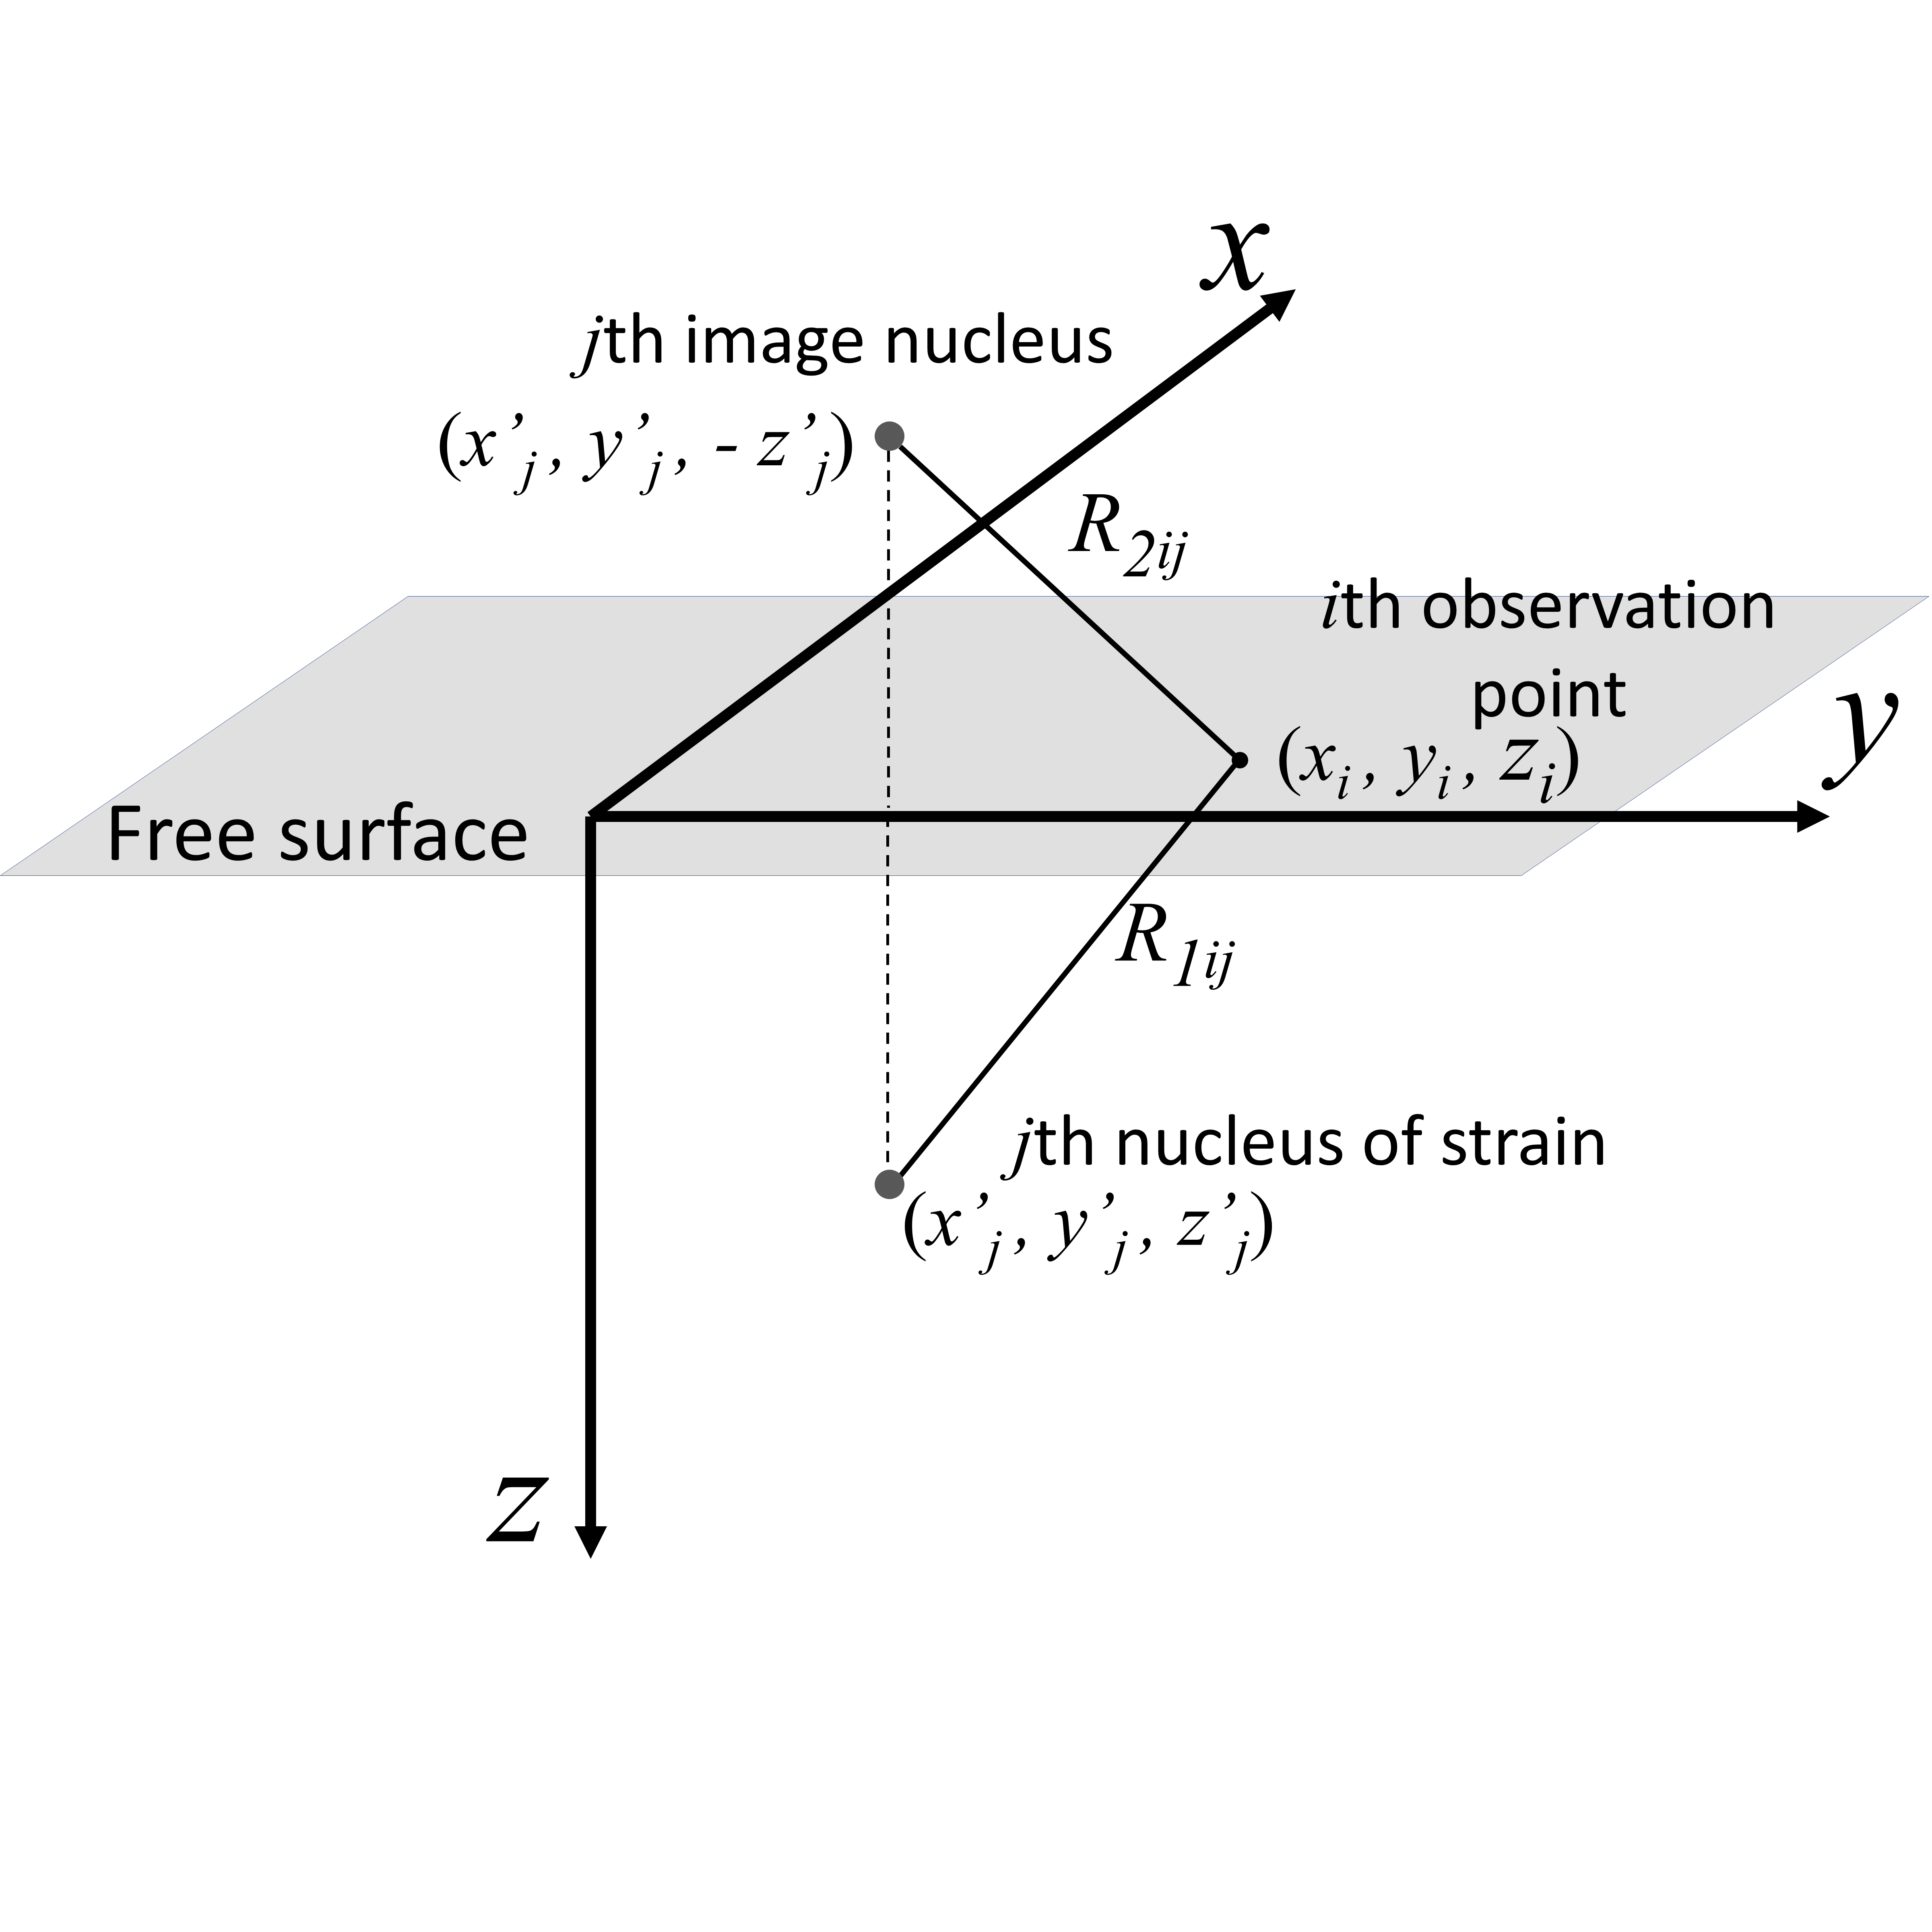
\includegraphics[width=8.3cm]{Fig/Figure_Nucleus_Strain.png}
\caption{Schematic representation of the geometry of the nucleus of strain in a semi-infinite medium. After \cite{Munoz&Roehl17}. 
The adopted Cartesian coordinate system considered the $x-$axis pointing to north, the $y-$axis pointing to east and the $z-$axis pointing downward.} 
\label{fig:nucleus_strain}
\end{figure}

%%% First Test: Disk-shaped reservoir under non uniform depletion

\begin{figure}[ht]
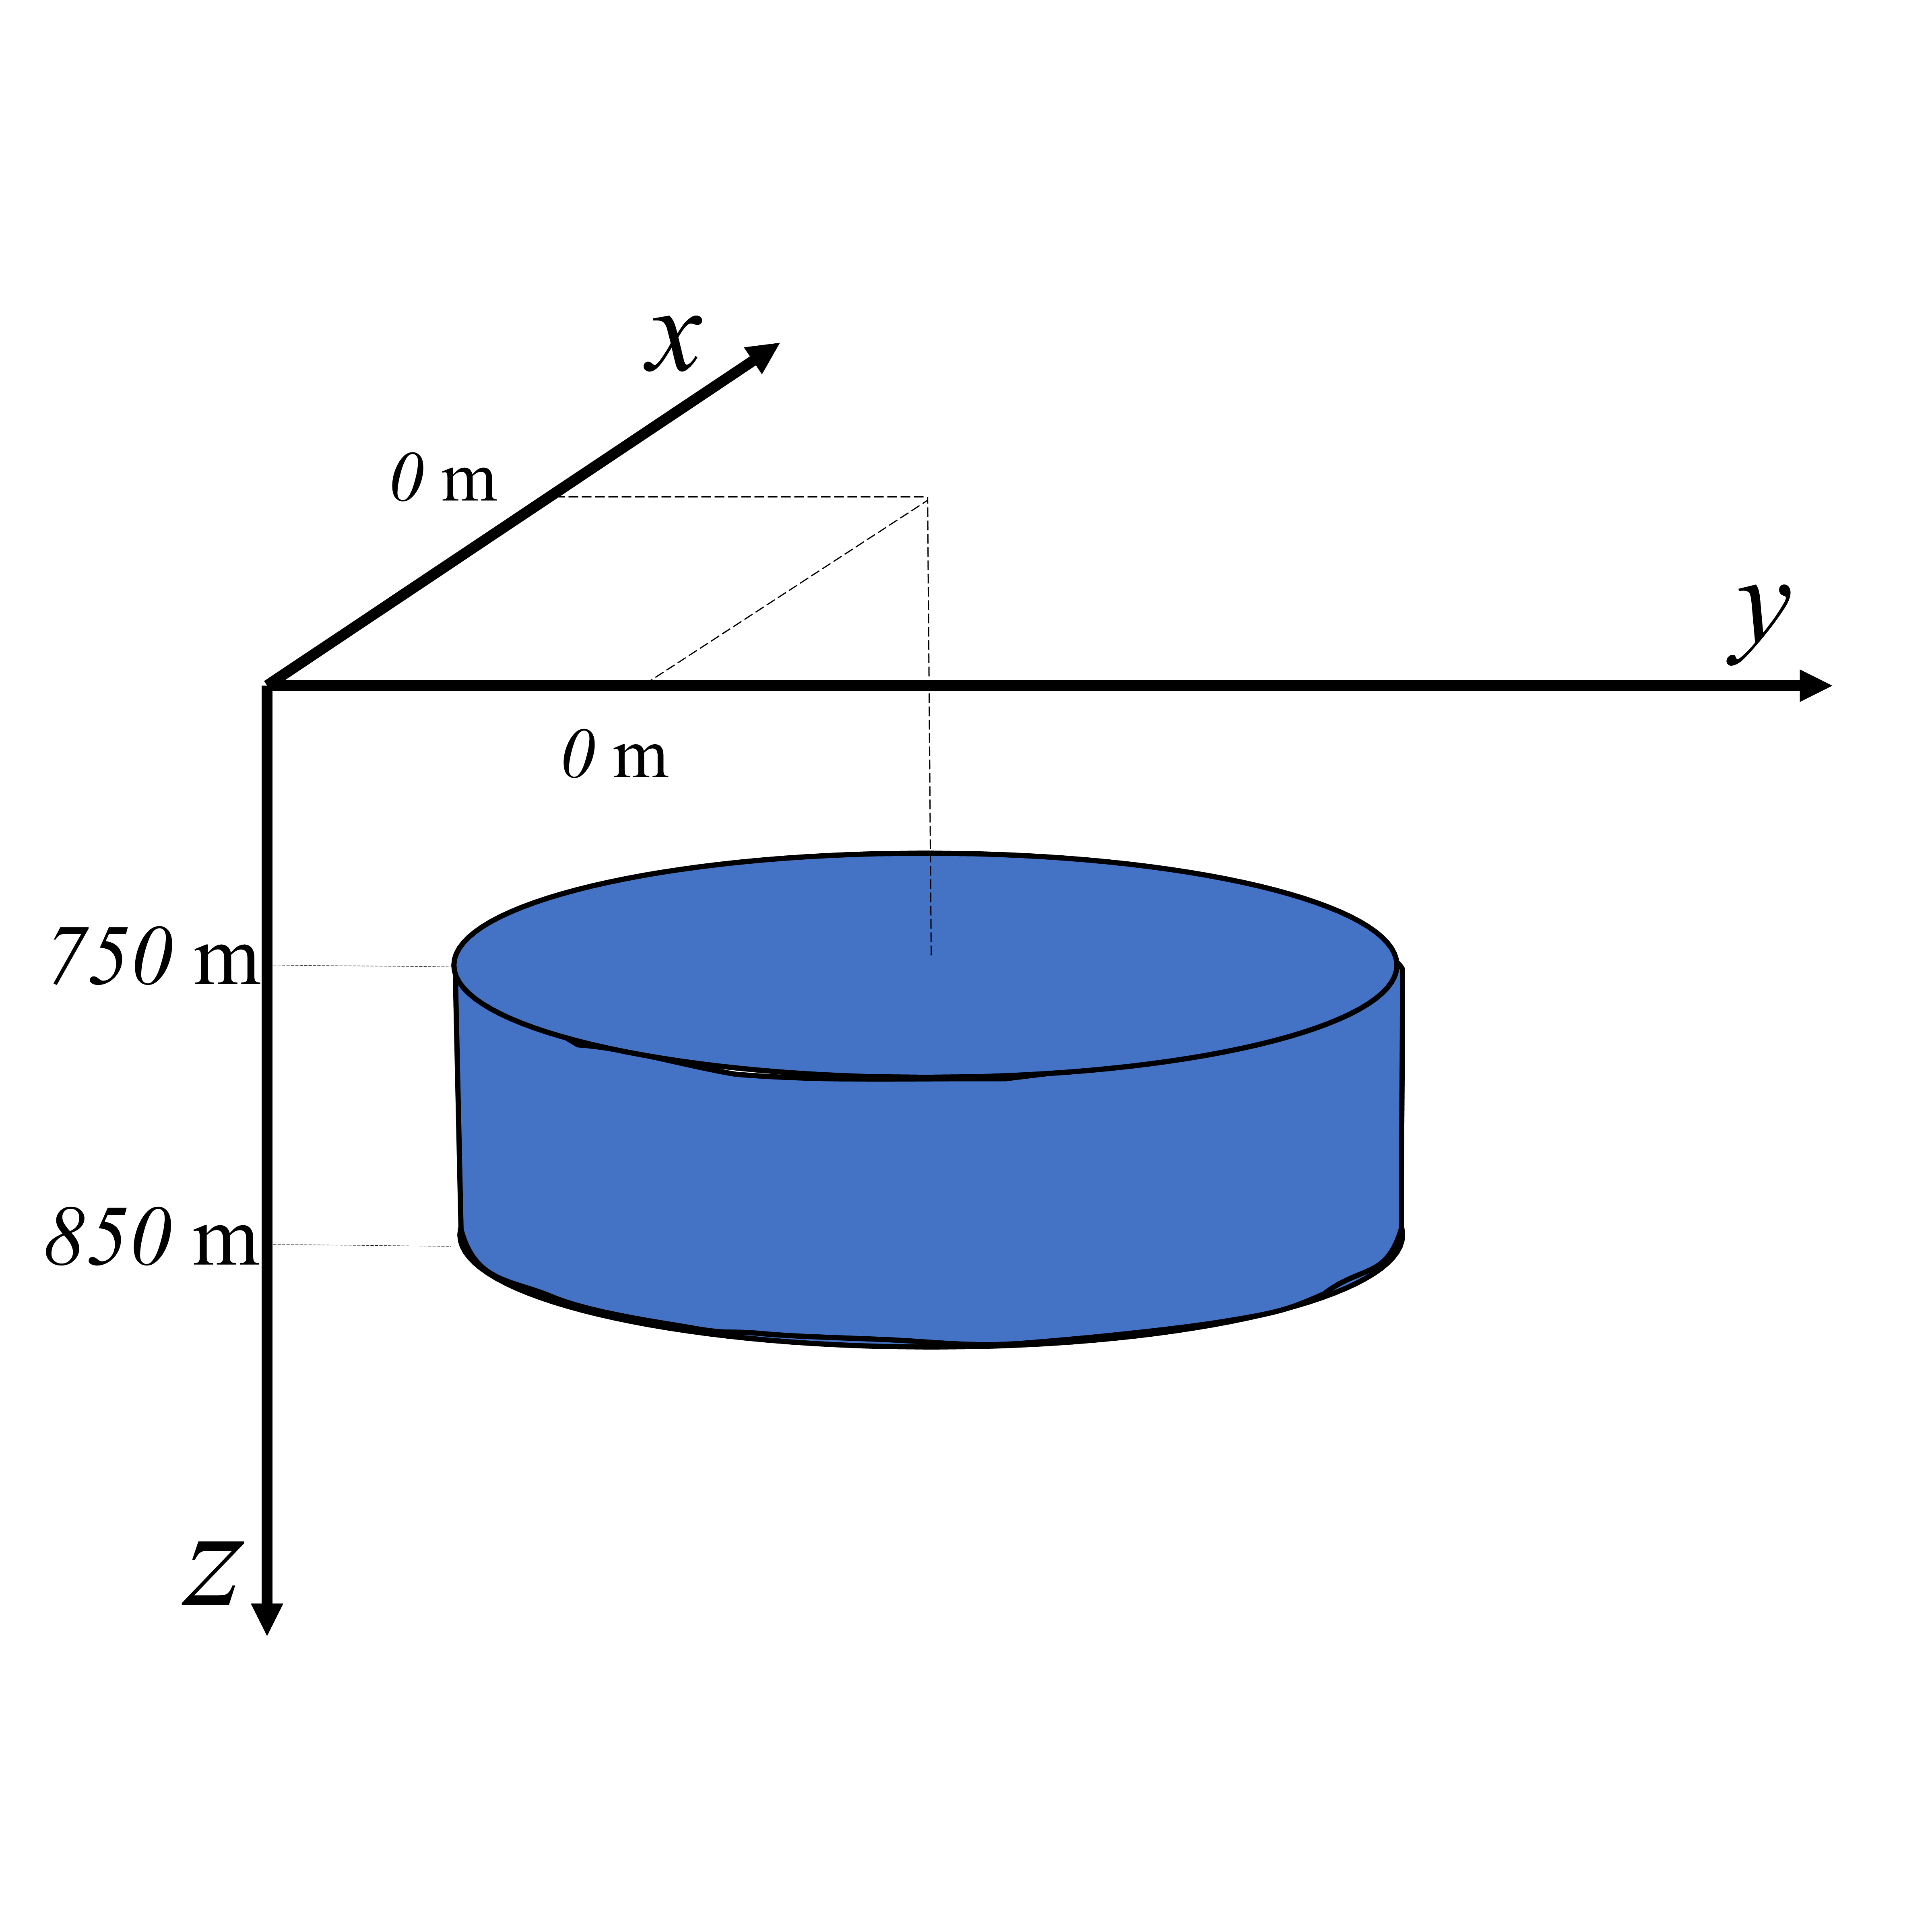
\includegraphics[width=8.3cm]{Fig/Figure_Cylinder.png}
\caption{Disk-shaped reservoir under uniform depletion with a radius of 500 m}
\label{fig:cylinder}
\end{figure}

\begin{figure}[ht]
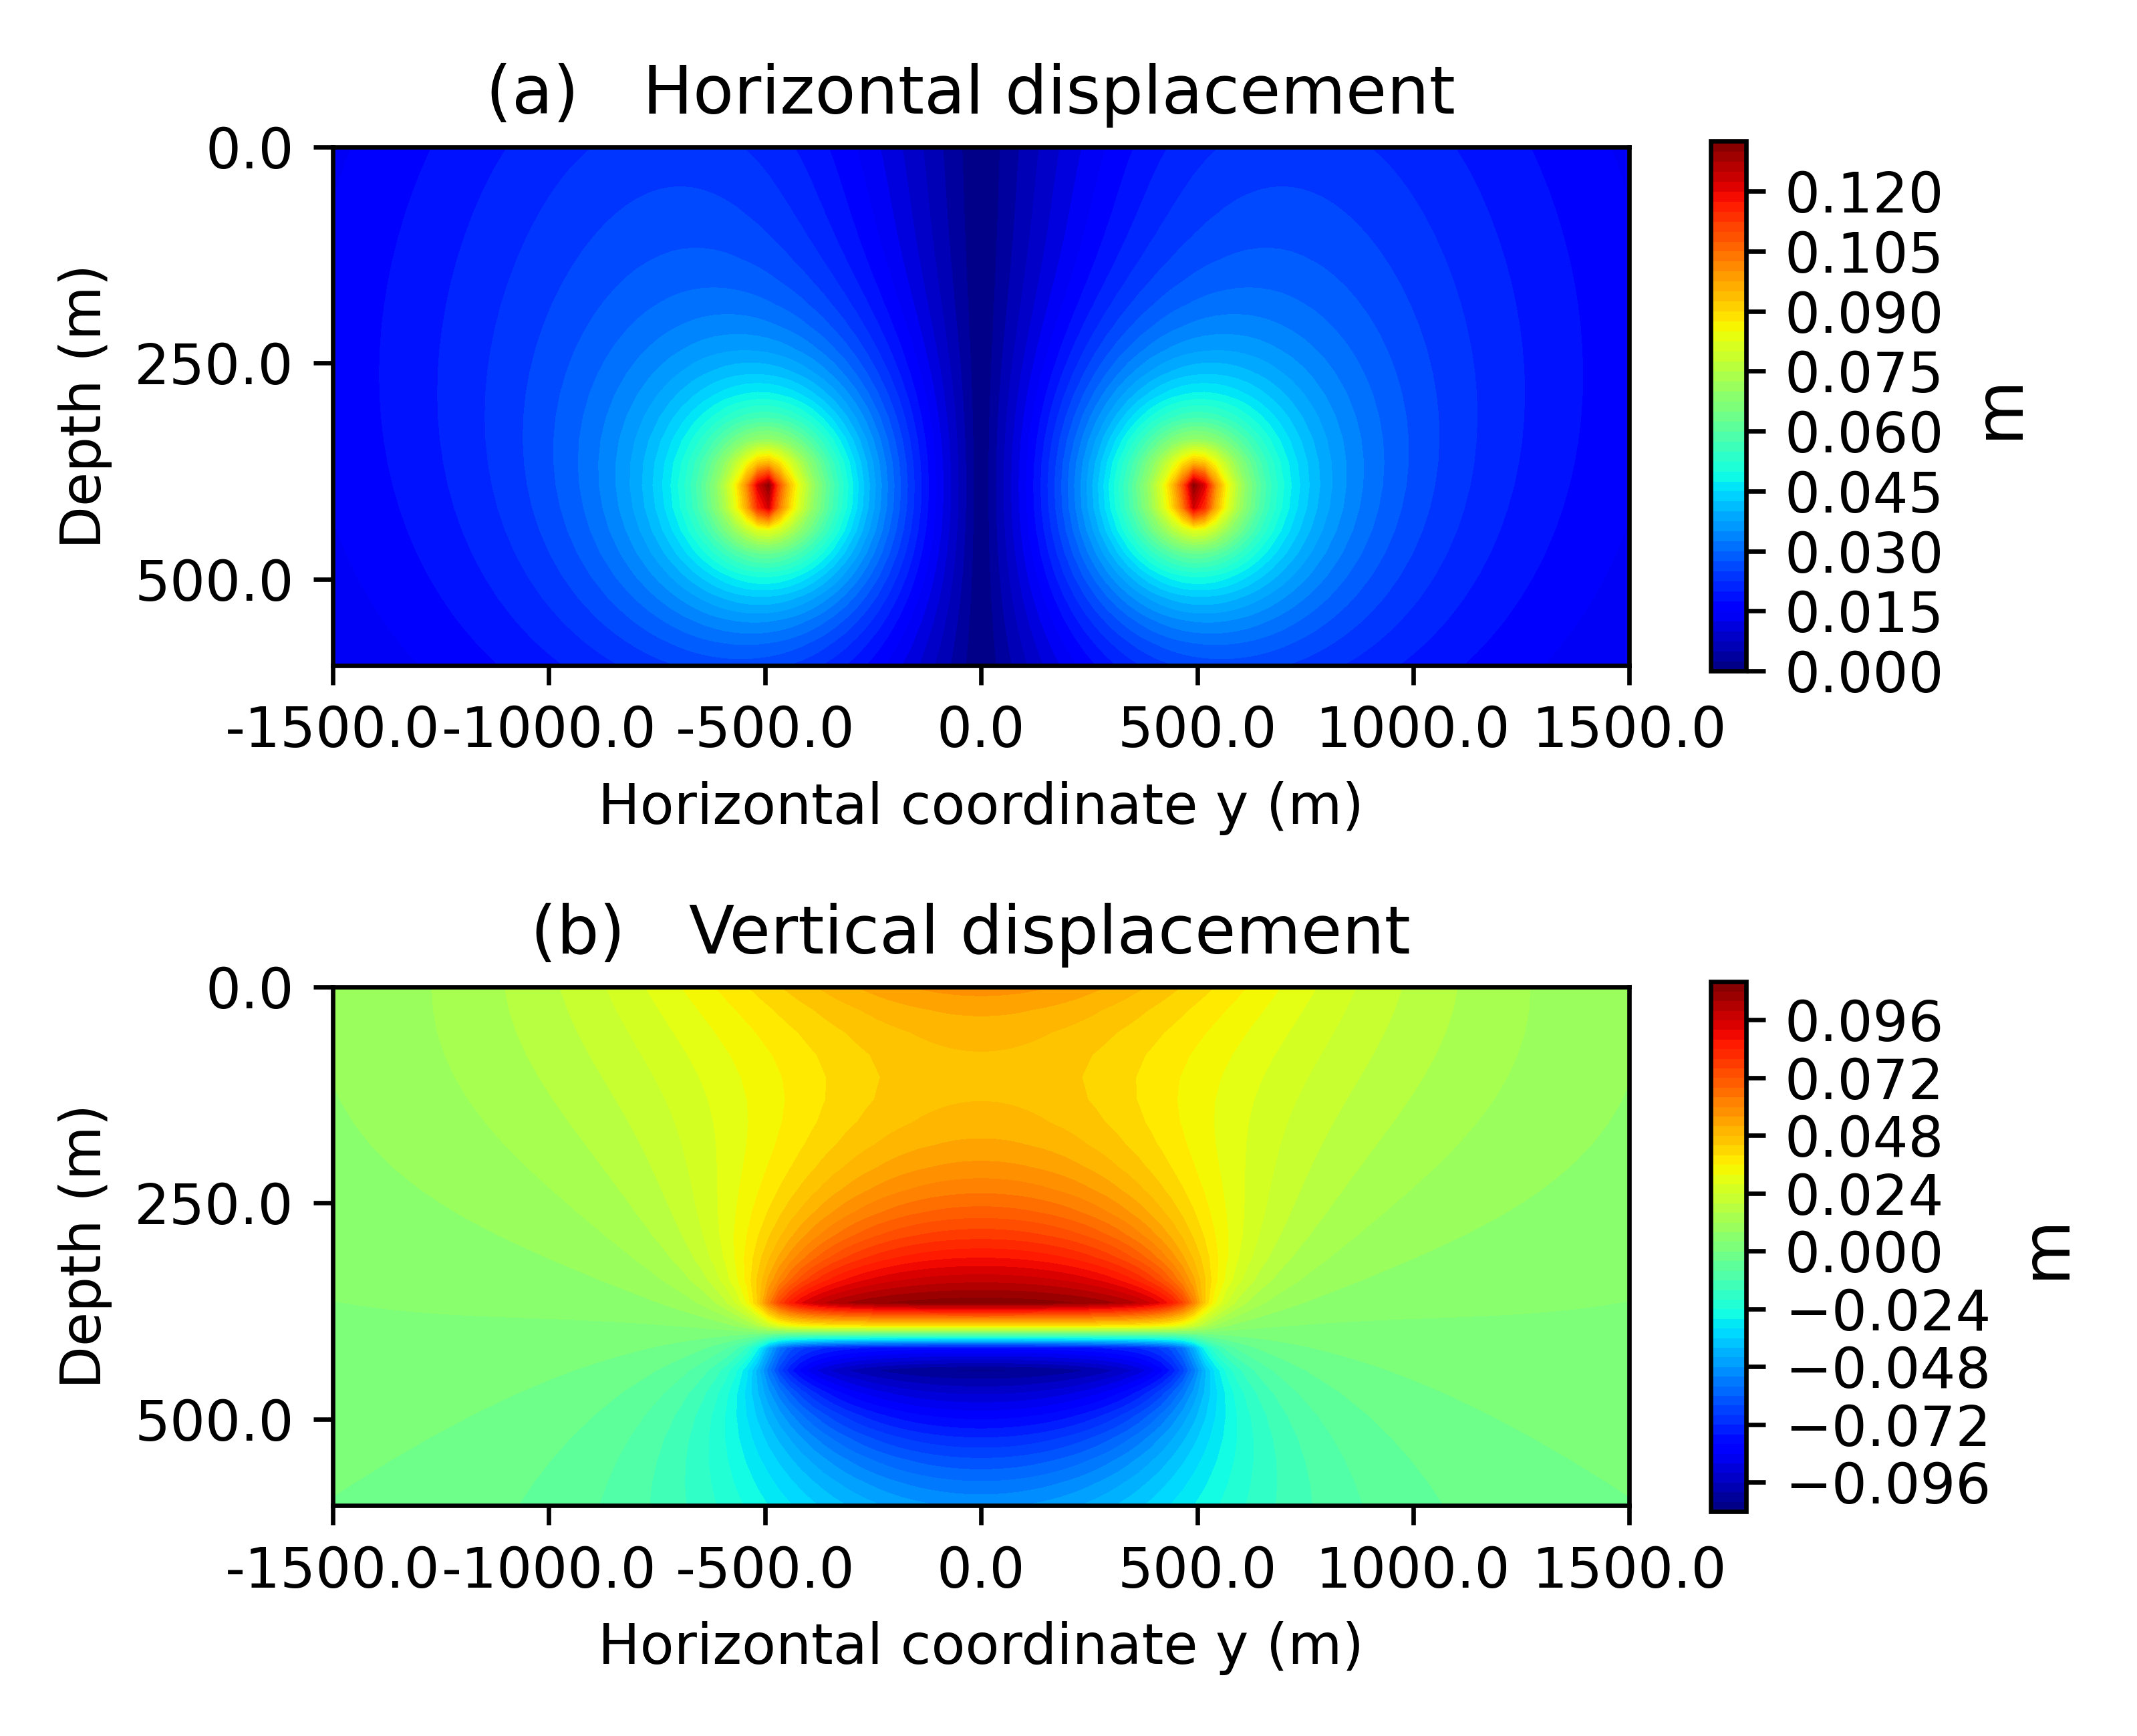
\includegraphics[width=8.3cm]{Fig/Figure_Displacement.png}
\caption{Reservoir under uniform depletion: (a) Horizontal displacement (equation \ref{eq:horizontal_displacement}) and (b) vertical displacement (equation \ref{eq:u_til_z}) by our methodology that uses the closed expressions of the volume integrations given by \cite{Nagyetal2000} and \cite{Nagyetal2002} (equations \ref{dx1}-\ref{dzz2})}
\label{fig:displacement}
\end{figure}

\begin{figure}[h]
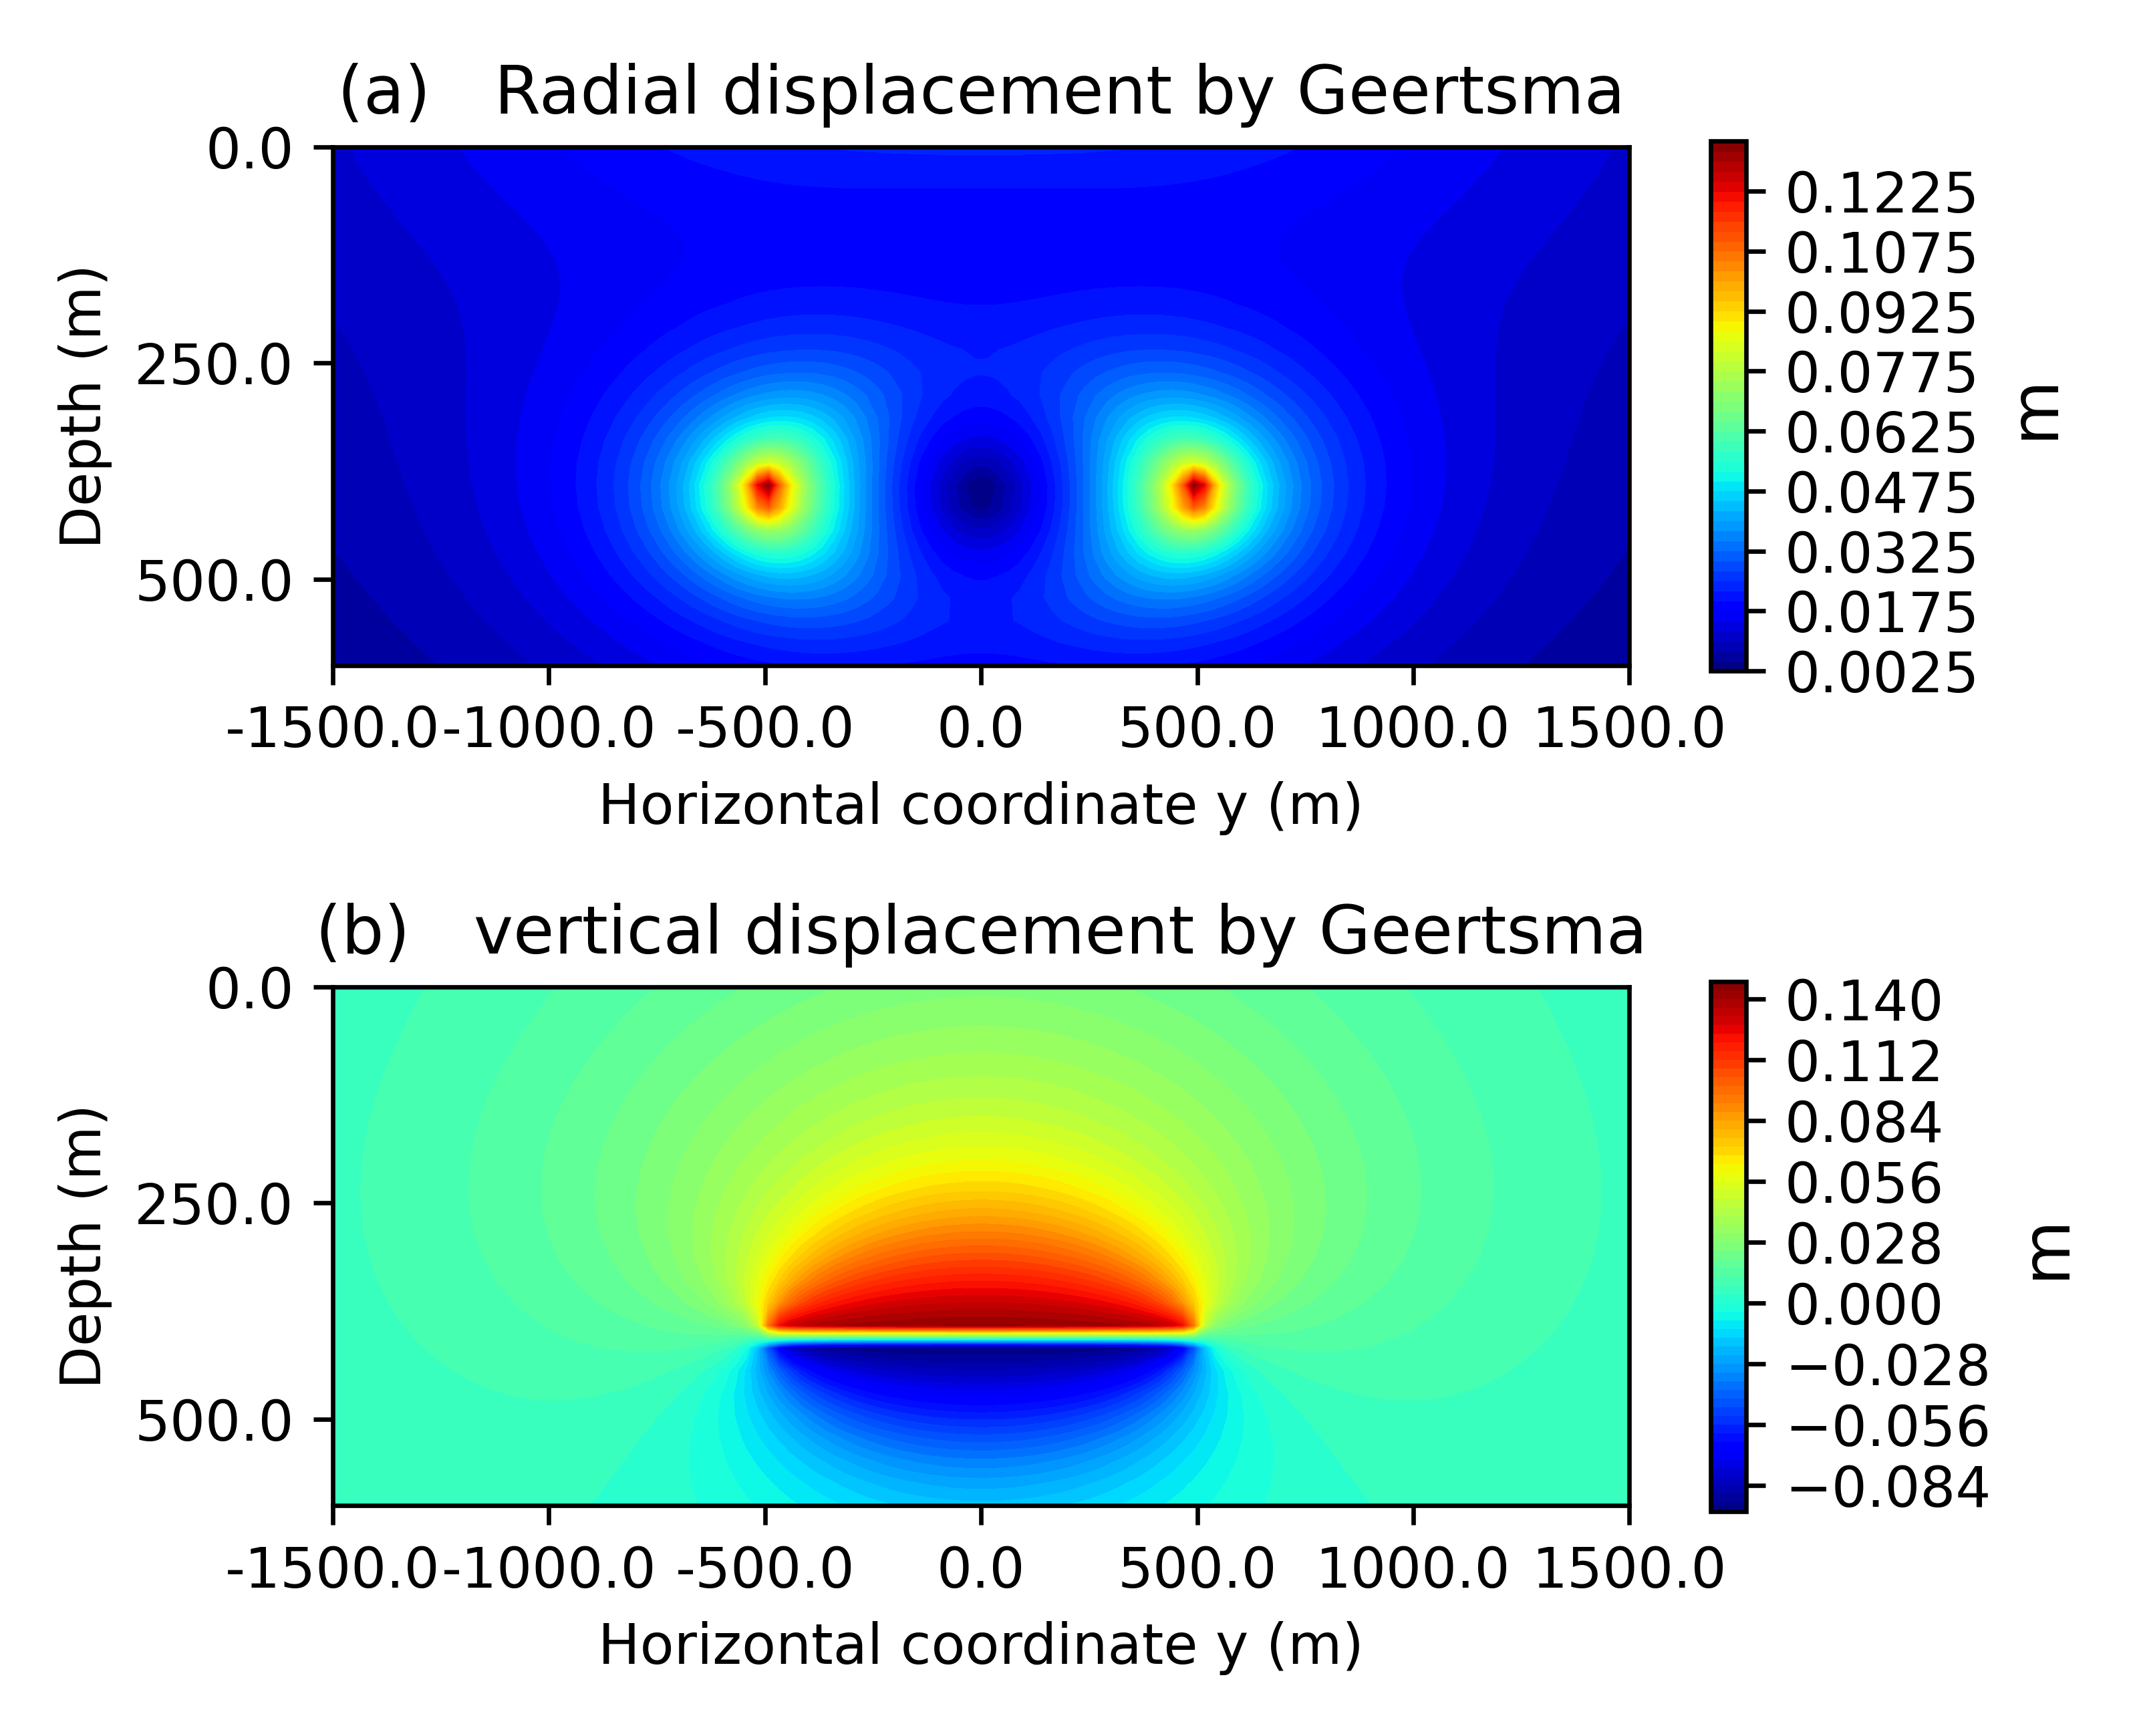
\includegraphics[width=8.3cm]{Fig/Figure_Displacement_Geertsma.png}
\caption{Reservoir under uniform depletion: (a) Radial displacement and (b) vertical displacement using Geertsma’s method \citep{Geertsma73}  considering an elastic homogeneous cylindrical reservoir under uniform depletion \citep{Fjaer08}}
\label{fig:displacement_Geertsma}
\end{figure}

\begin{figure}[ht]
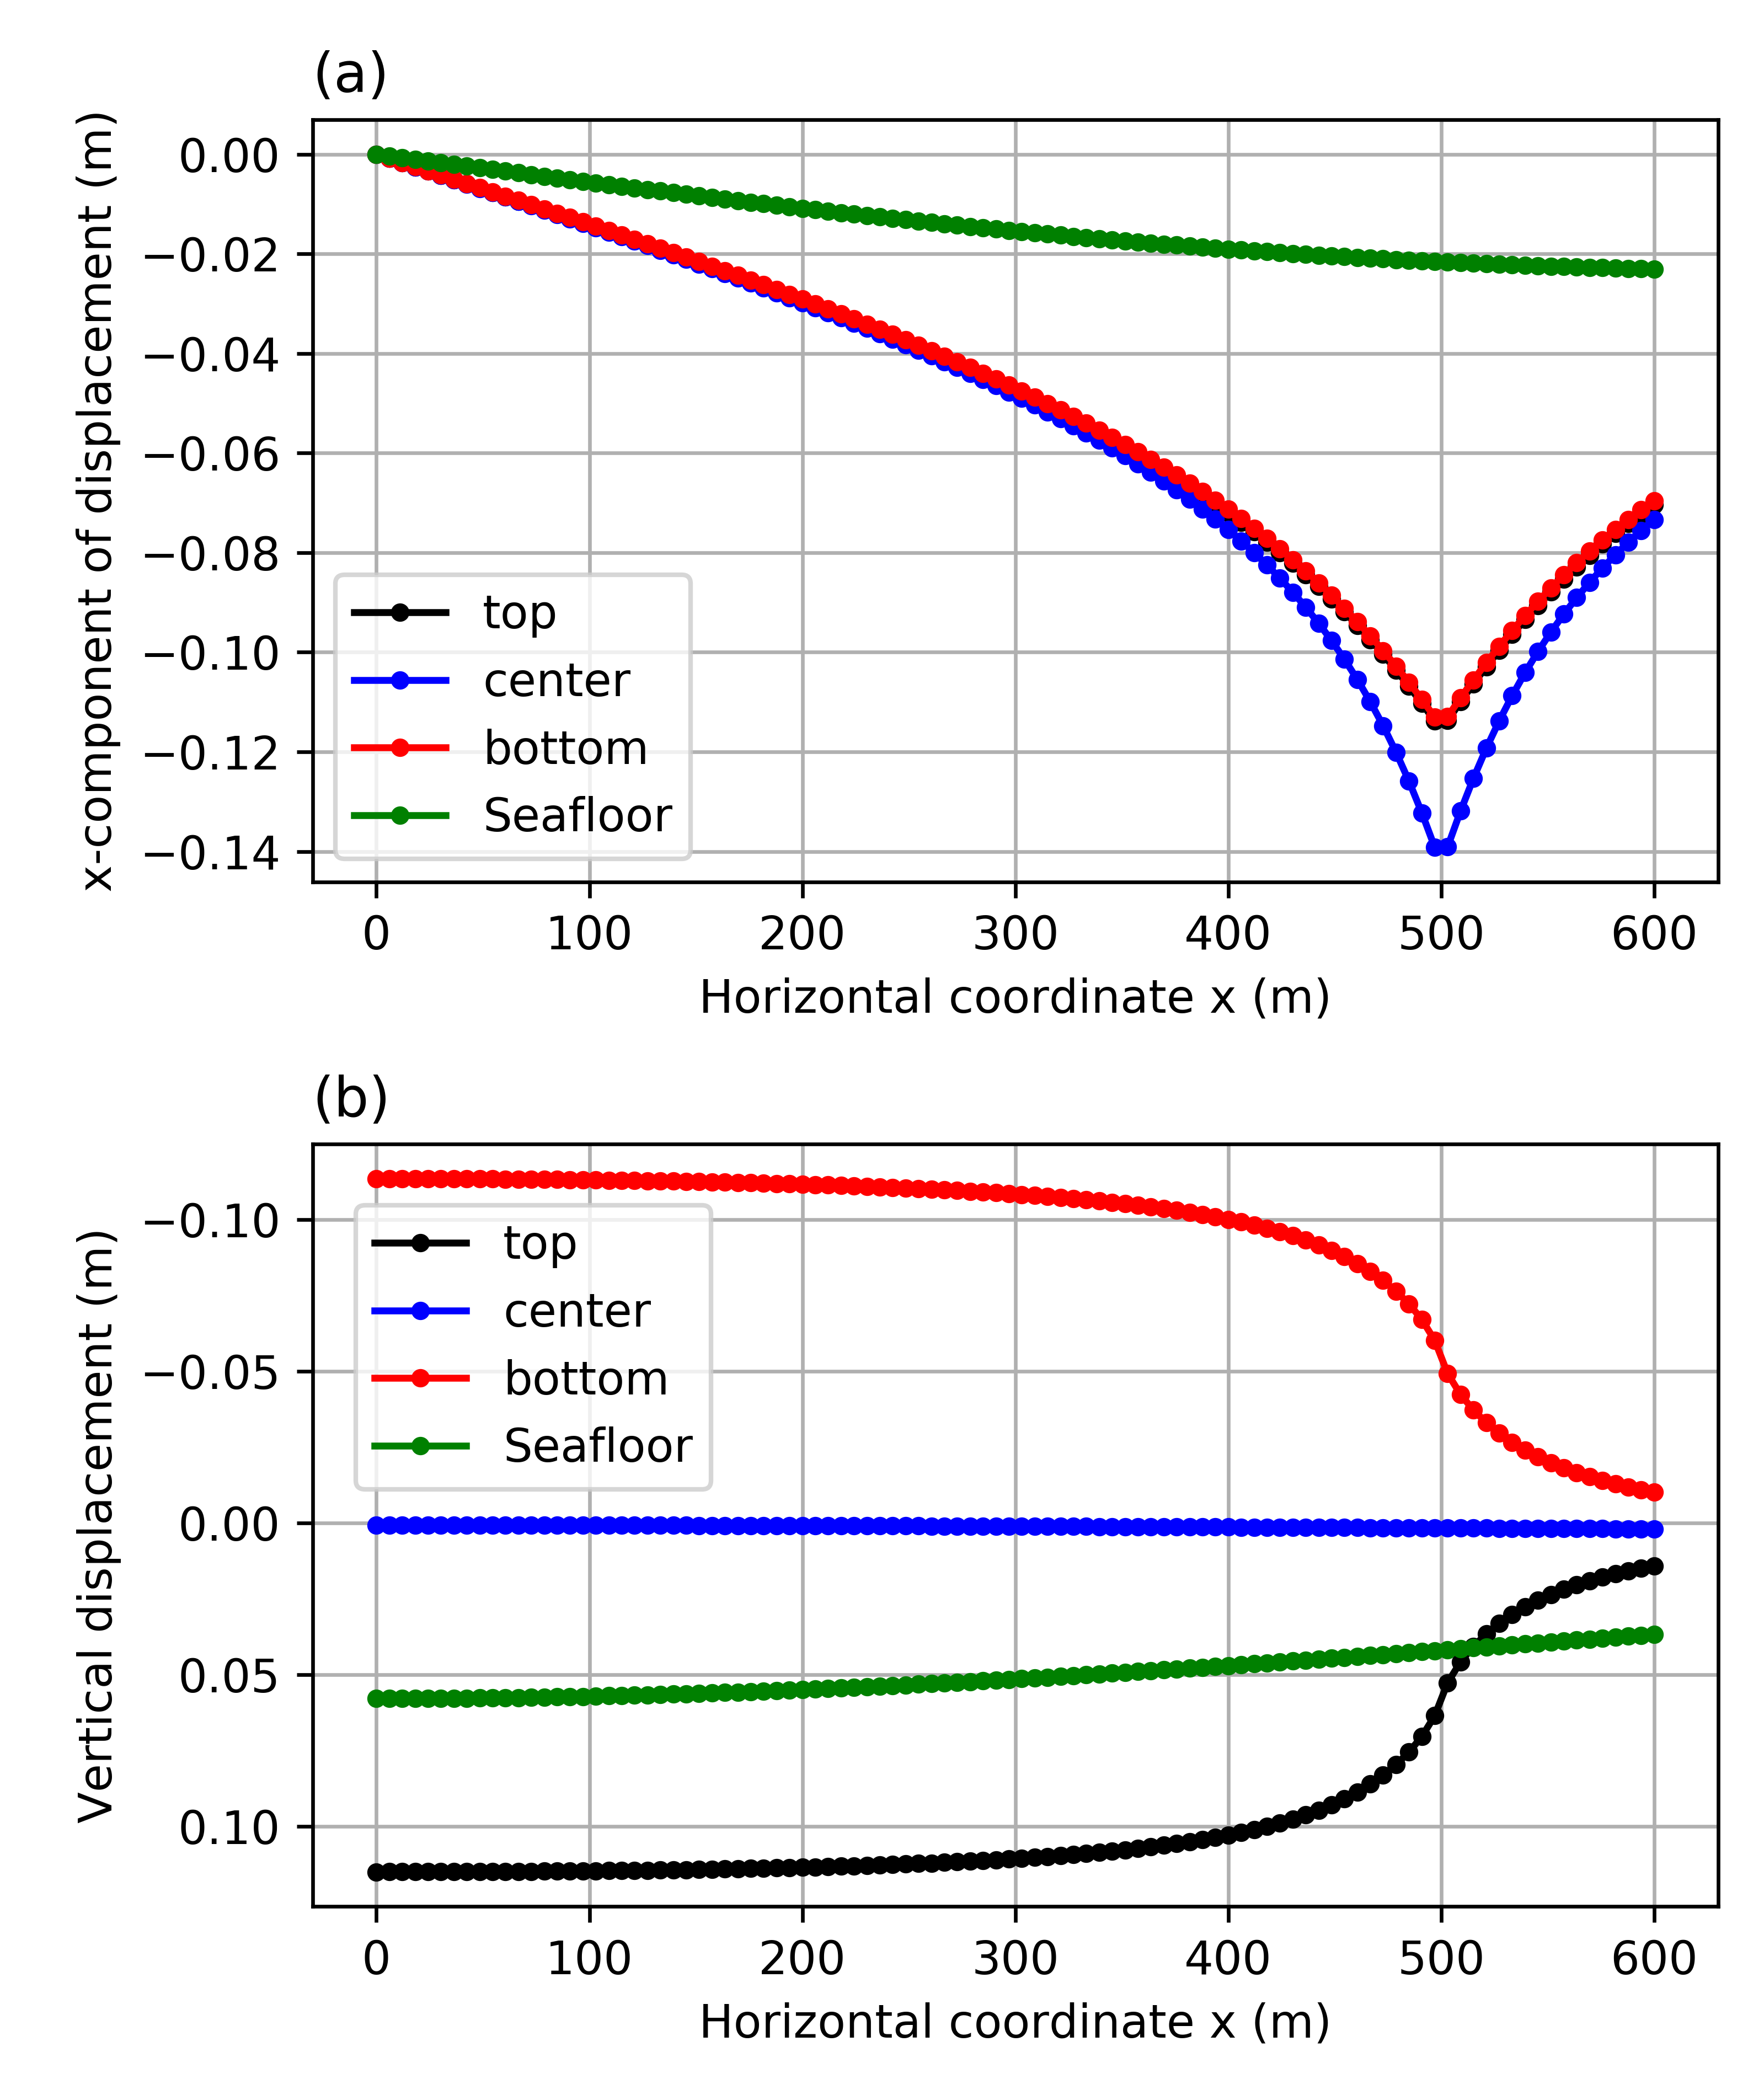
\includegraphics[width=8.3cm]{Fig/Figure_Displacement_z_levels.png}
\caption{Reservoir under uniform depletion: (a) Horizontal x-component displacement and (b) vertical displacement by our methodology that uses the closed expressions of the volume integrations given by \cite{Nagyetal2000} and \cite{Nagyetal2002} (equations \ref{dx1}-\ref{dzz2}).
These displacements are calculated along the x-axis, at $y = 0$ m and $z$ located at the depths of:  seafloor ($z = 0$ m), reservoir top ($z = 750$ m), reservoir center ($z = 800$ m) and reservoir bottom ($z = 850$ m).}
\label{fig:displacement_z_levels}
\end{figure}

\begin{figure}[ht]
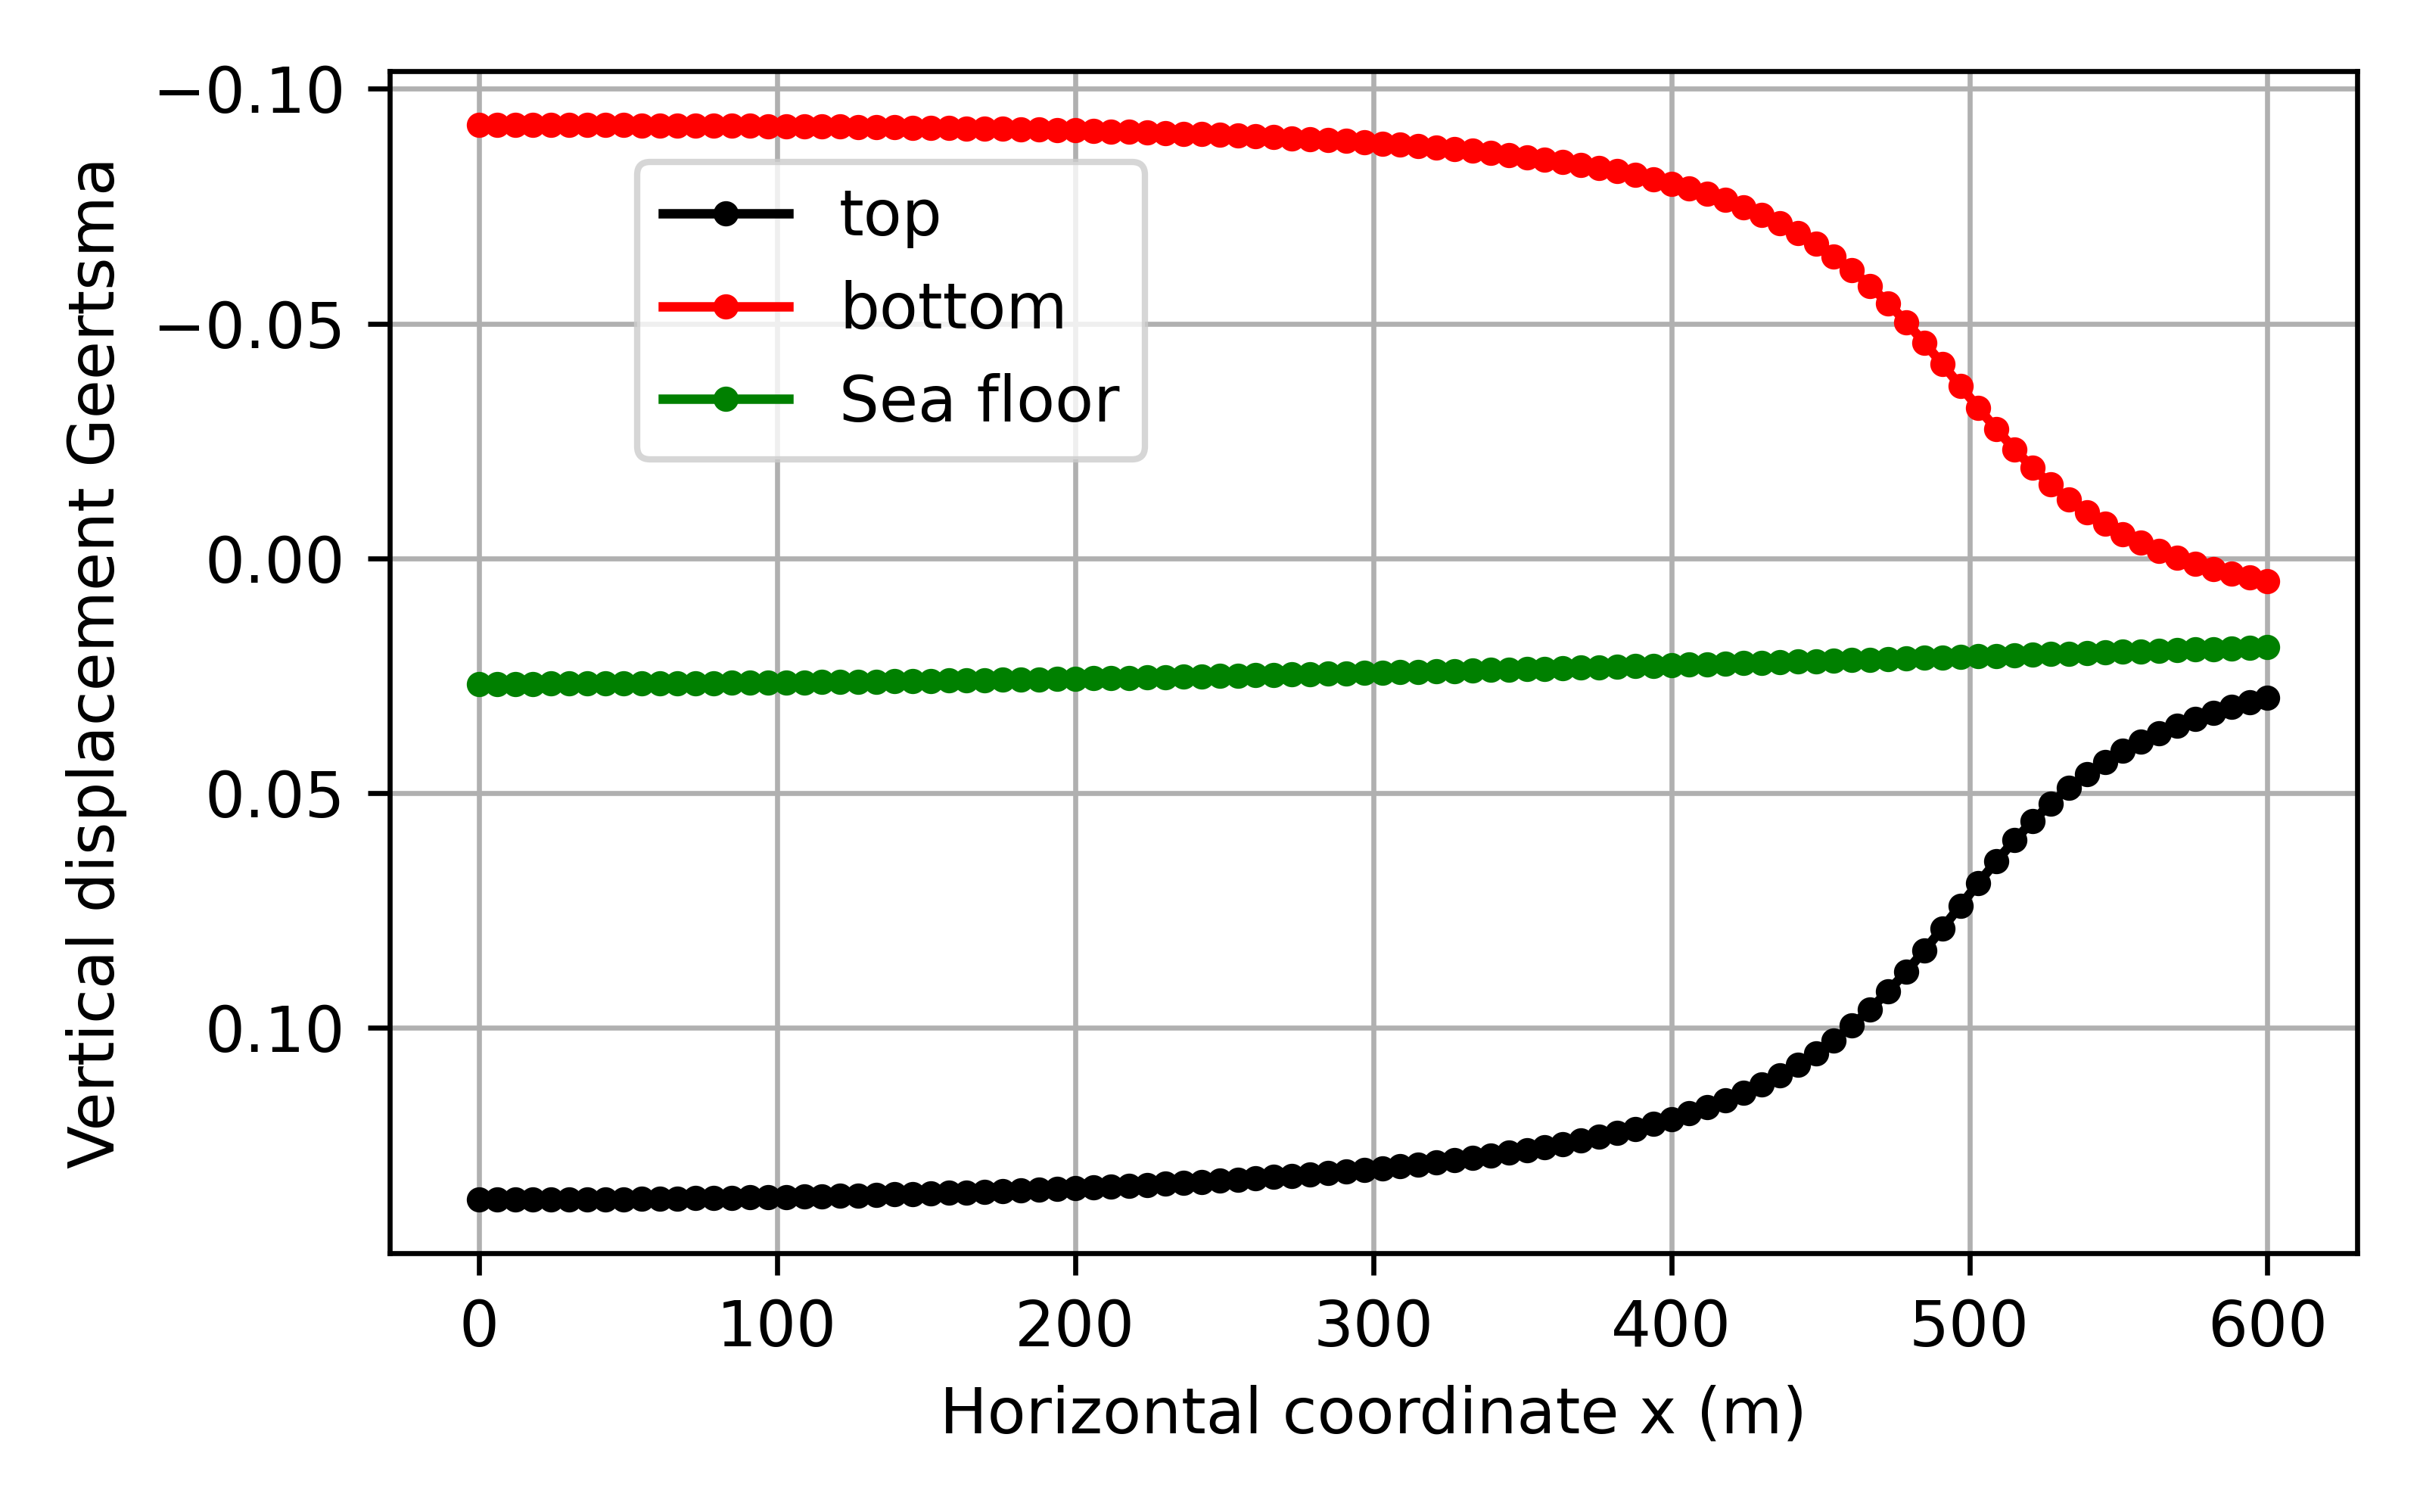
\includegraphics[width=8.3cm]{Fig/Figure_Displacement_z_levels_Geertsma.png}
\caption{Reservoir under uniform depletion: Vertical displacement using Geertsma’s method \citep{Geertsma73}  considering an elastic homogeneous cylindrical reservoir under uniform depletion \citep{Fjaer08}.
The displacement is calculated along the x-axis, at $y = 0$ m and $z$ located at the depths of:  seafloor ($z = 0$ m), reservoir top ($z = 750$ m), and reservoir bottom 
($z = 850$ m).}
\label{fig:displacement_z_levels_Geertsma}
\end{figure}


\begin{figure}[ht]
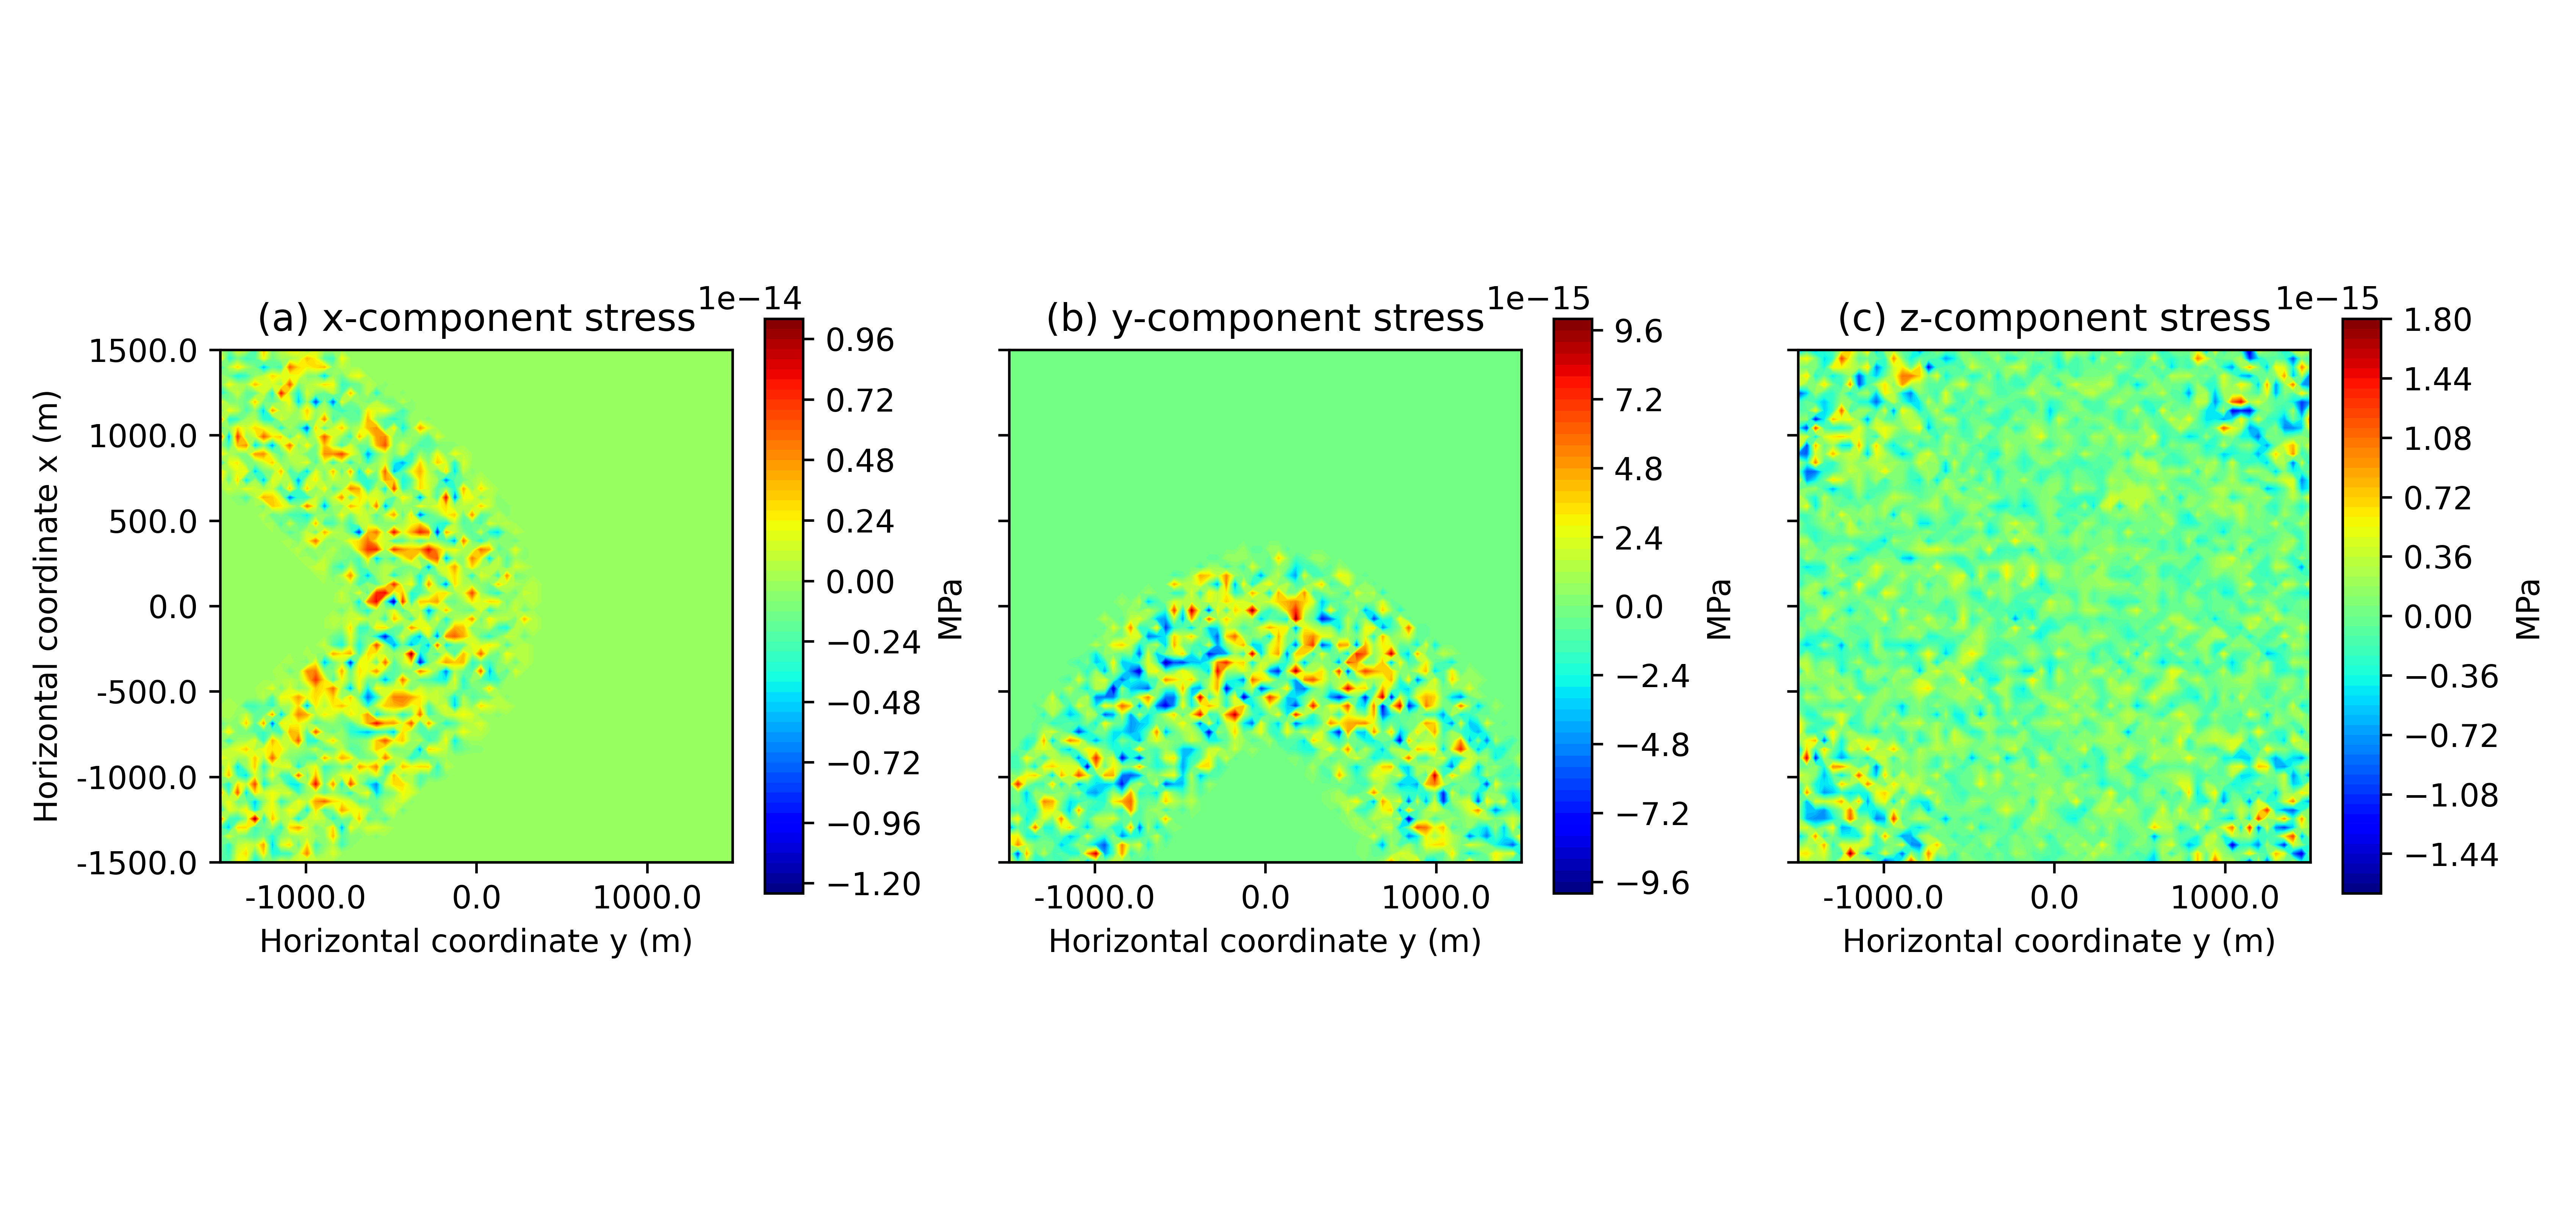
\includegraphics[width=12cm]{Fig/Figure_Null_stress.png}
\caption{Reservoir under uniform depletion: (a) $x-$, (b) $y-$, and (c) $z-$components of the stress at the free surface.}
\label{fig:Null_stress}
\end{figure}


%%% Second test: Disk-shaped reservoir under non uniform depletion


\begin{figure}[ht]
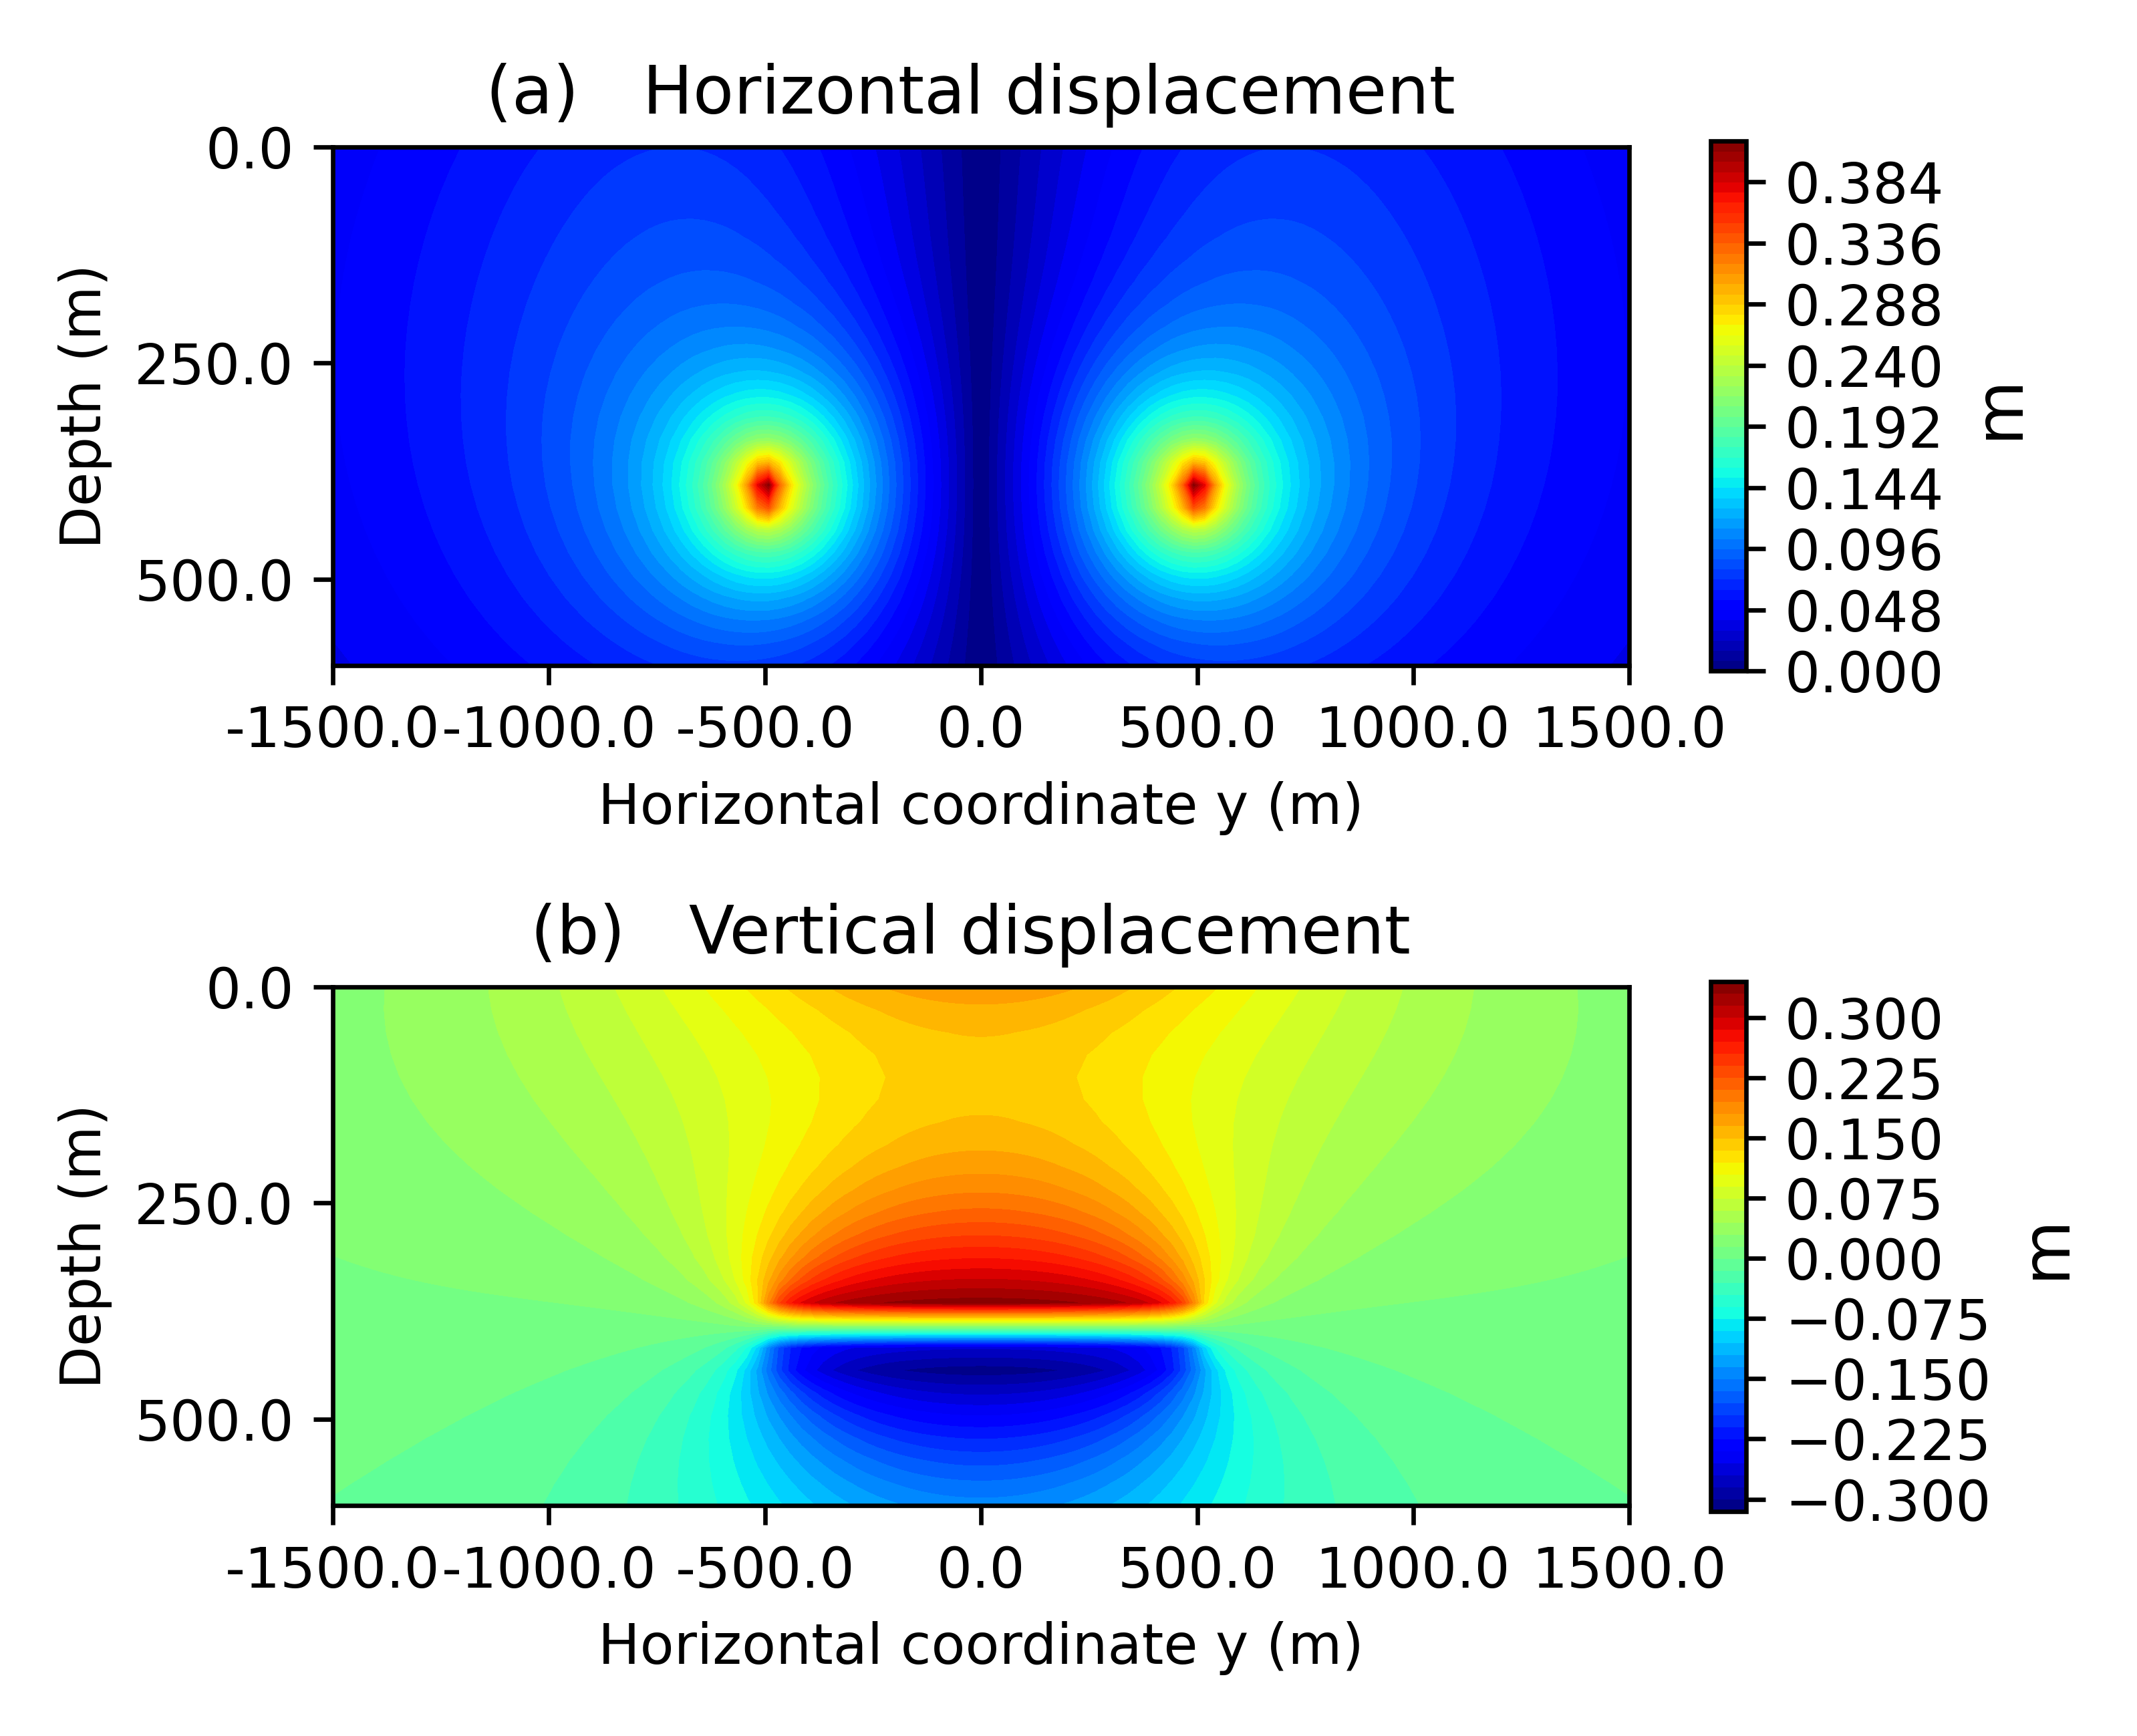
\includegraphics[width=8.3cm]{Fig/Figure_Displacement_non_uniform_depletion.png}
\caption{Reservoir under non uniform depletion: (a) Horizontal displacement (equation \ref{eq:horizontal_displacement}) and (b) vertical displacement (equation \ref{eq:u_til_z}) by our methodology that uses the closed expressions of the volume integrations given by \cite{Nagyetal2000} and \cite{Nagyetal2002} (equations \ref{dx1}--\ref{dzz2})}
\label{fig:displacement_non_uniform_depletion}
\end{figure}

\begin{figure}[ht]
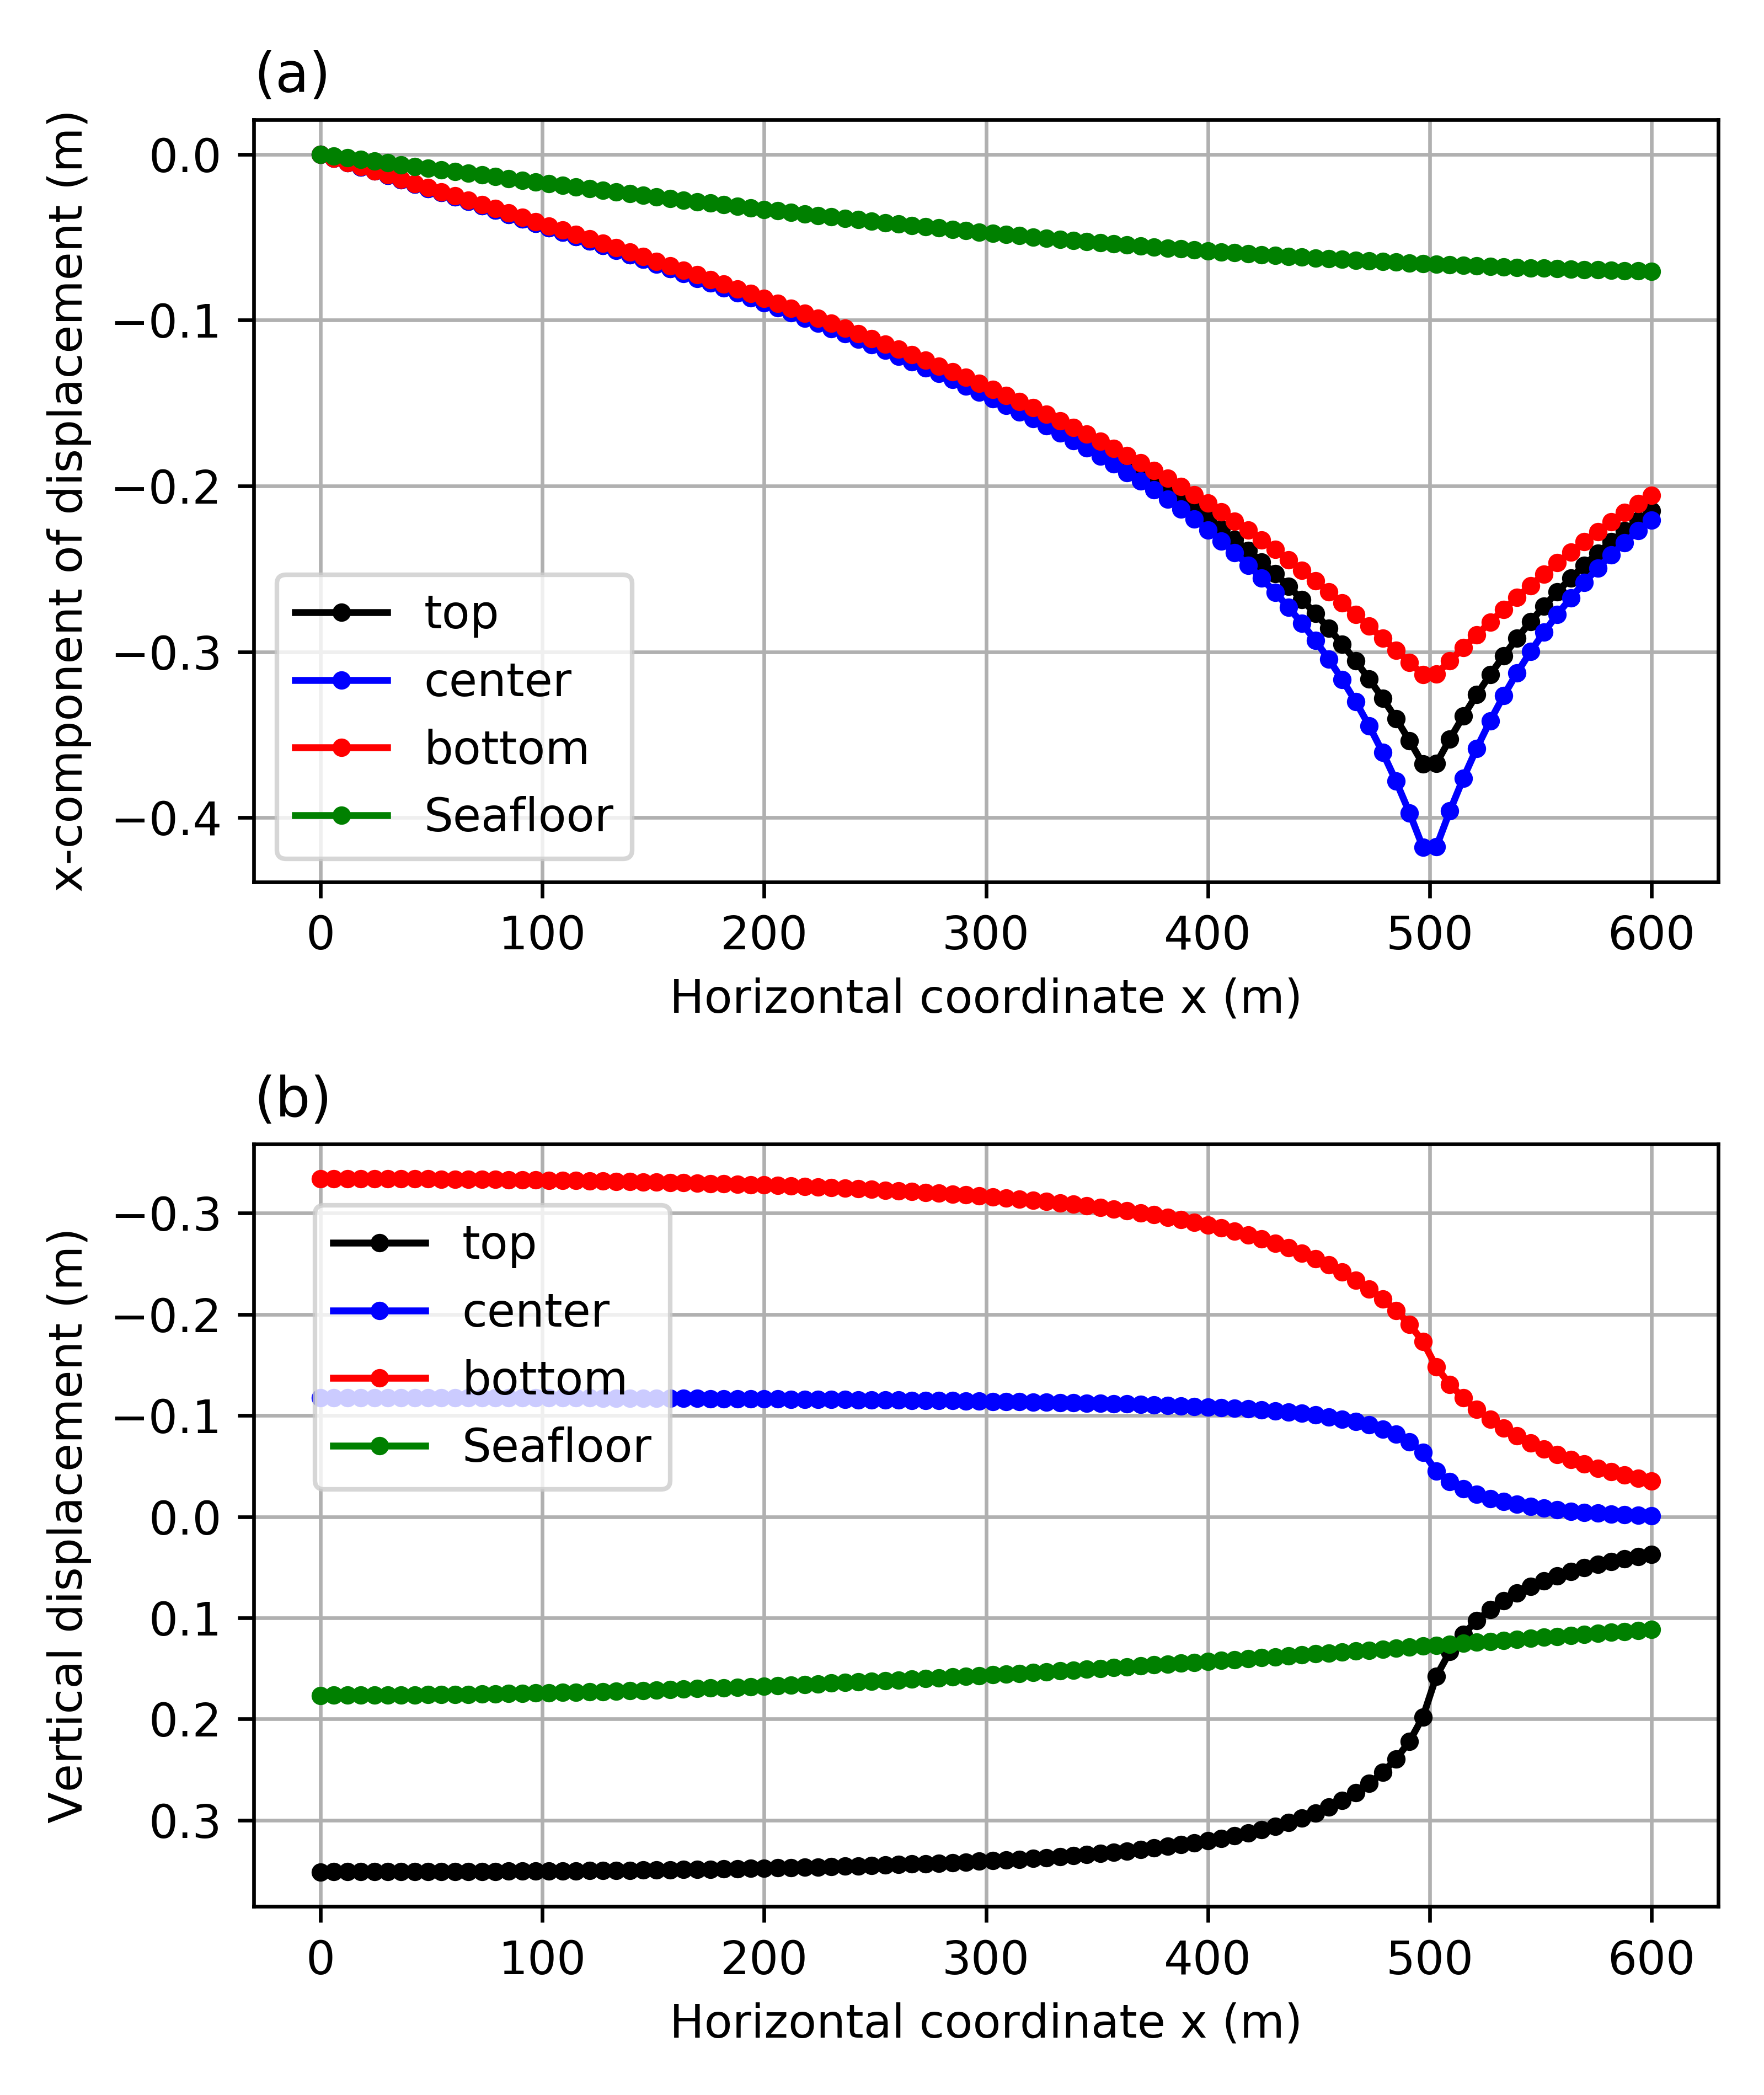
\includegraphics[width=8.3cm]{Fig/Figure_Displacement_z_levels_non_uniform_depletion.png}
\caption{Reservoir under non uniform depletion: (a) Horizontal x-component displacement and (b) vertical displacement by our methodology that uses the closed expressions of the volume integrations given by \cite{Nagyetal2000} and \cite{Nagyetal2002} (equations \ref{dx1}--\ref{dzz2}).
These displacements are calculated along the x-axis, at $y = 0$ m and $z$ located at the depths of:  seafloor ($z = 0$ m), reservoir top ($z = 750$ m), reservoir center ($z = 800$ m) and reservoir bottom ($z = 850$ m).}
\label{fig:displacement_z_levels_non_uniform_depletion}
\end{figure}


\begin{figure}[ht]
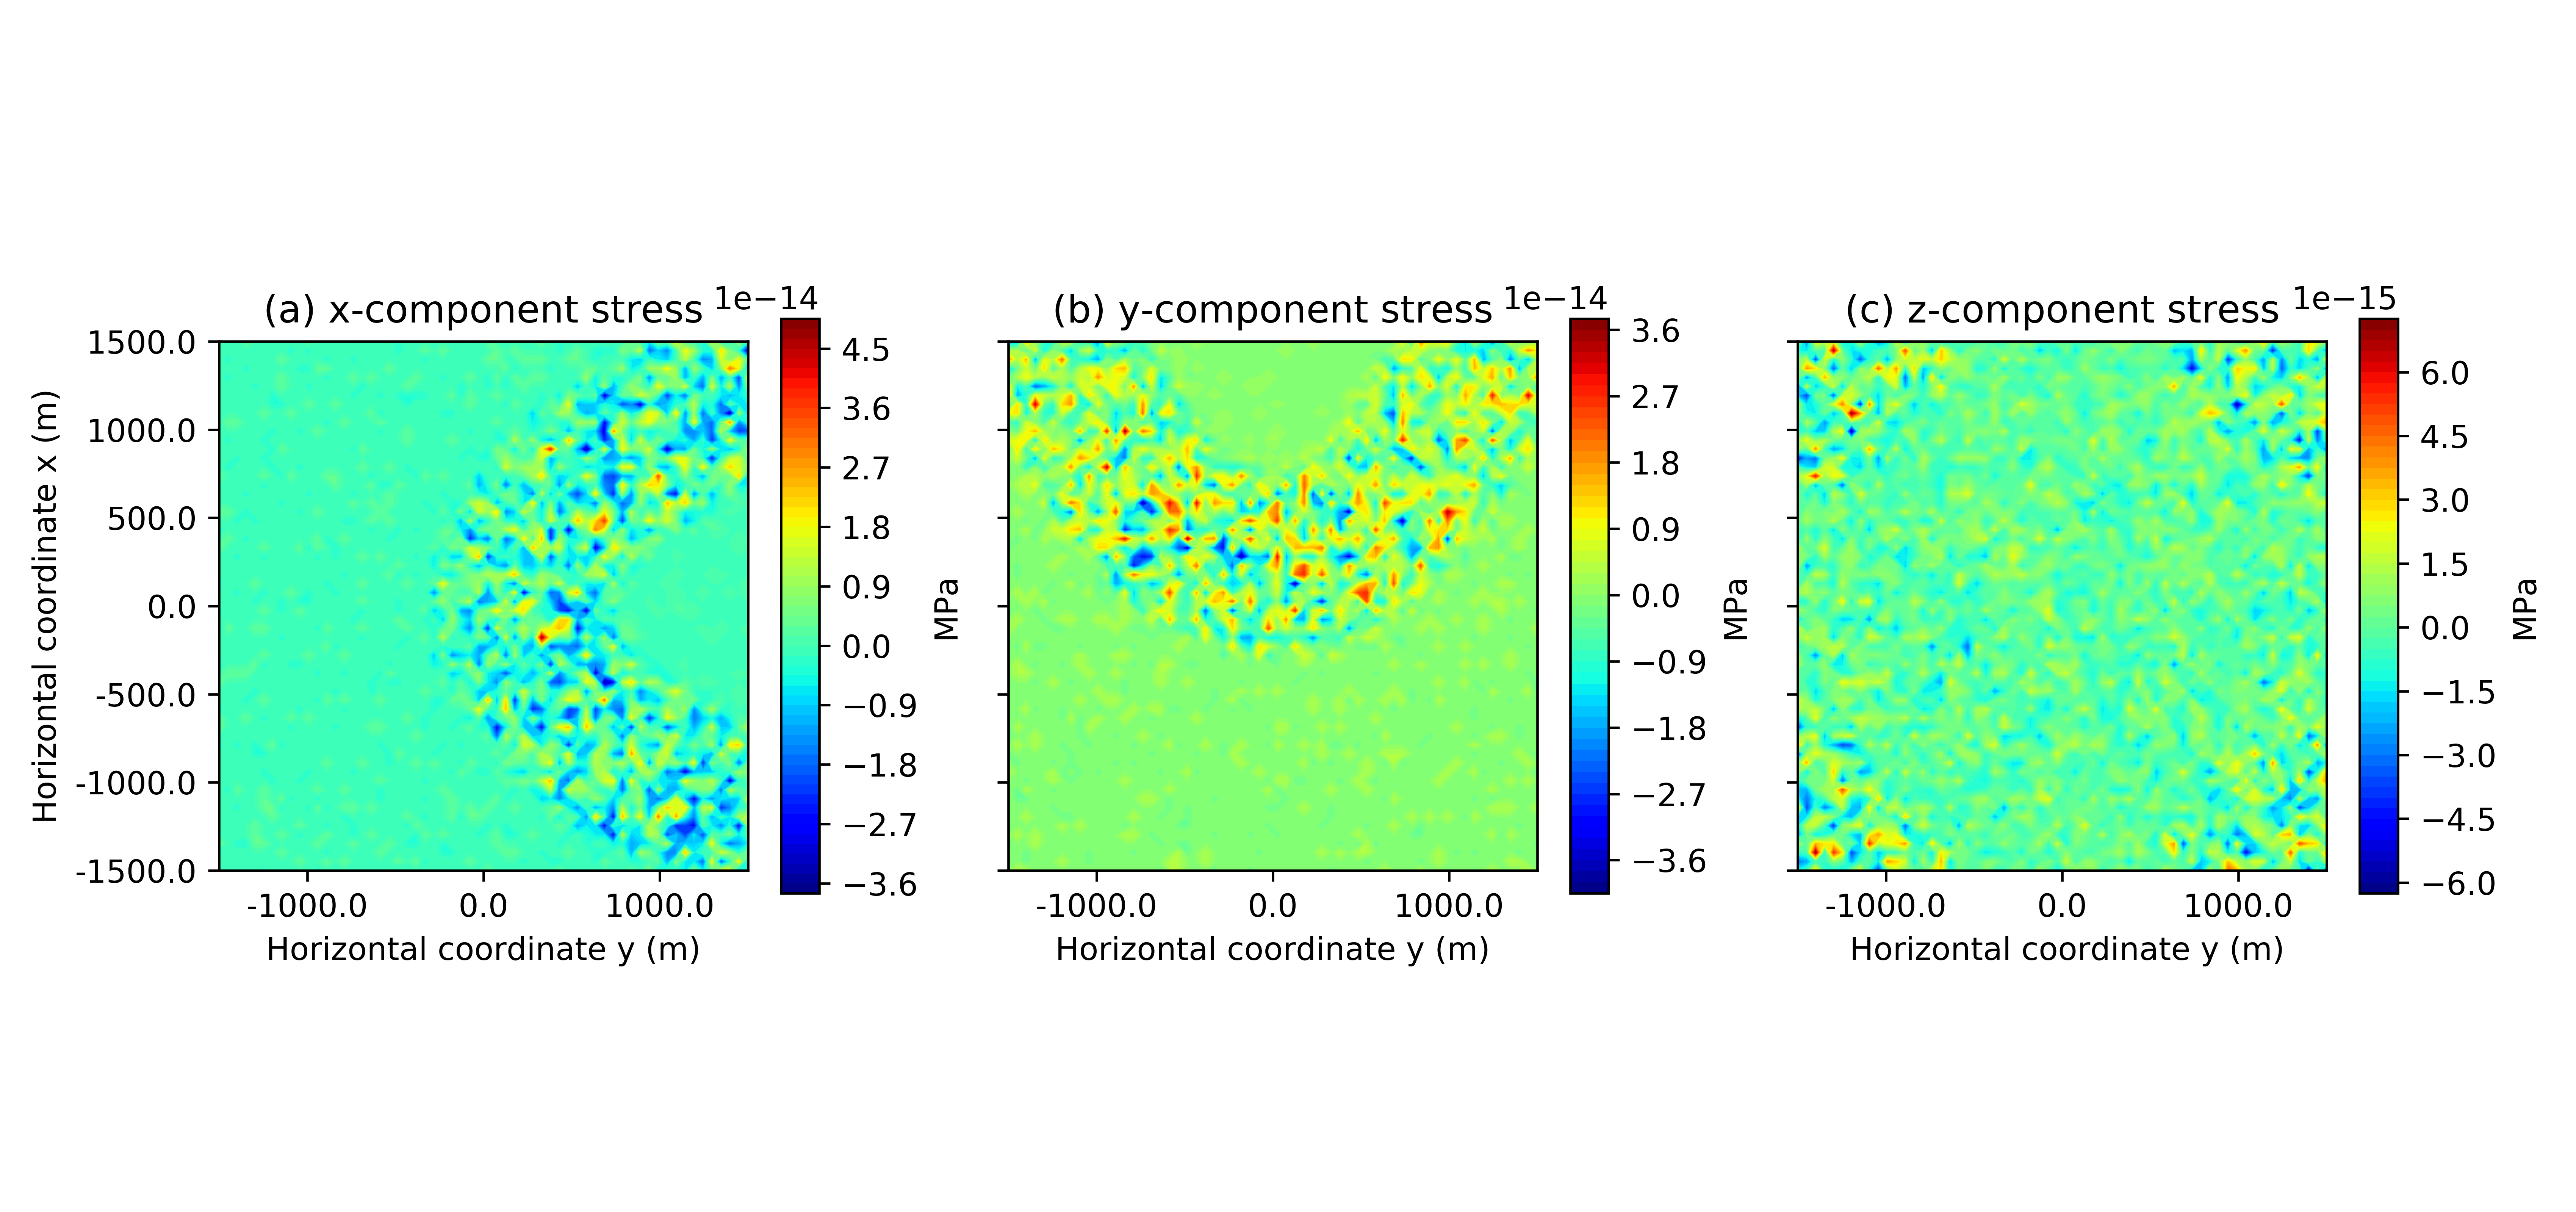
\includegraphics[width=12cm]{Fig/Figure_Null_stress_non_uniform_depletion.png}
\caption{Reservoir under non uniform depletion: (a) $x-$, (b) $y-$, and (c) $z-$components of the stress at the free surface.}
\label{fig:Null_stress_non_uniform_depletion}
\end{figure}

%% Third test: Reservoir with arbitrary geometry and under arbitrary pressure changes


\begin{figure}[ht]

\includegraphics[width=8.3cm]{Fig/Figure_Pressure_complex_reservoir.png}
\caption{Reservoir with arbitrary geometry and under arbitrary pressure changes: 3D perspective view of the pore pressure distribution of a realistic reservoir 
located in a production oil field in offshore Brazil.}
\label{fig:pressure_complex_reservoir}
\end{figure}

\begin{figure}[ht]
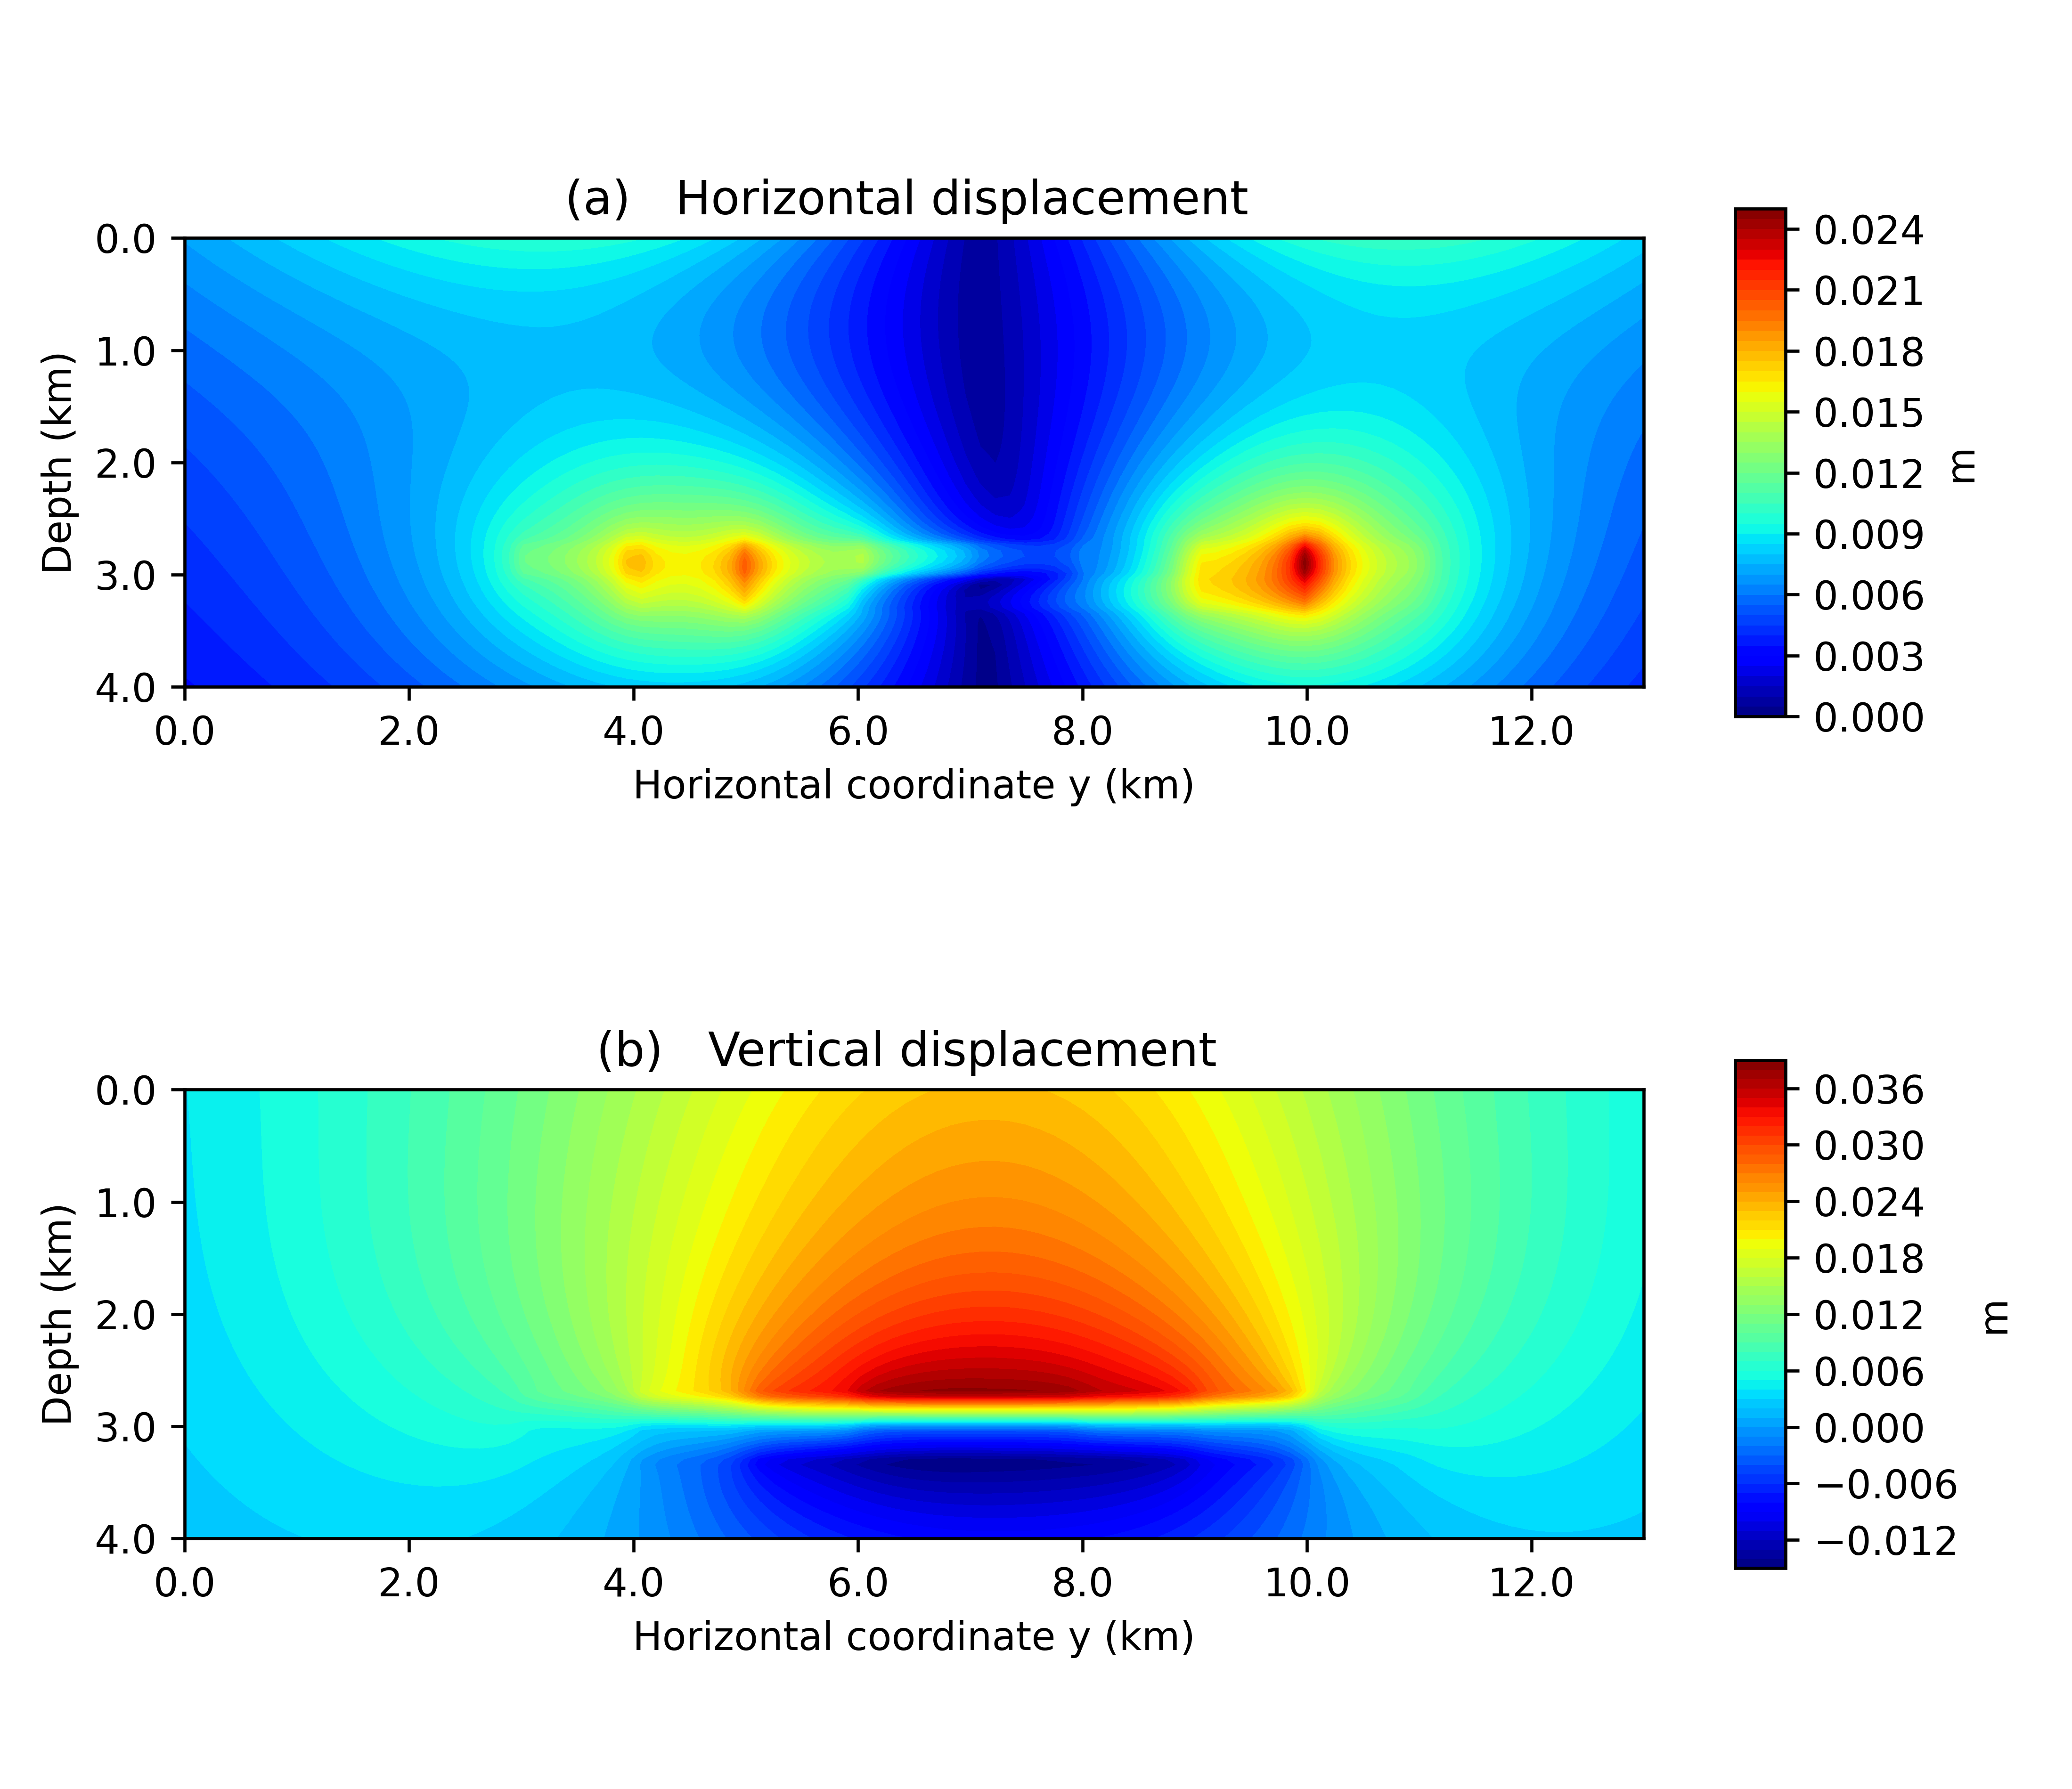
\includegraphics[width=8.3cm]{Fig/Figure_Displacement_complex_reservoir.png}
\caption{Reservoir with arbitrary geometry and under arbitrary pressure changes: (a) Horizontal displacement (equation \ref{eq:horizontal_displacement}) and (b) vertical displacement (equation \ref{eq:u_til_z}) by our methodology that uses the closed expressions of the volume integrations given by \cite{Nagyetal2000} and \cite{Nagyetal2002} (equations \ref{dx1}--\ref{dzz2})}
\label{fig:displacement_complex_reservoir}
\end{figure}

\begin{figure}[ht]
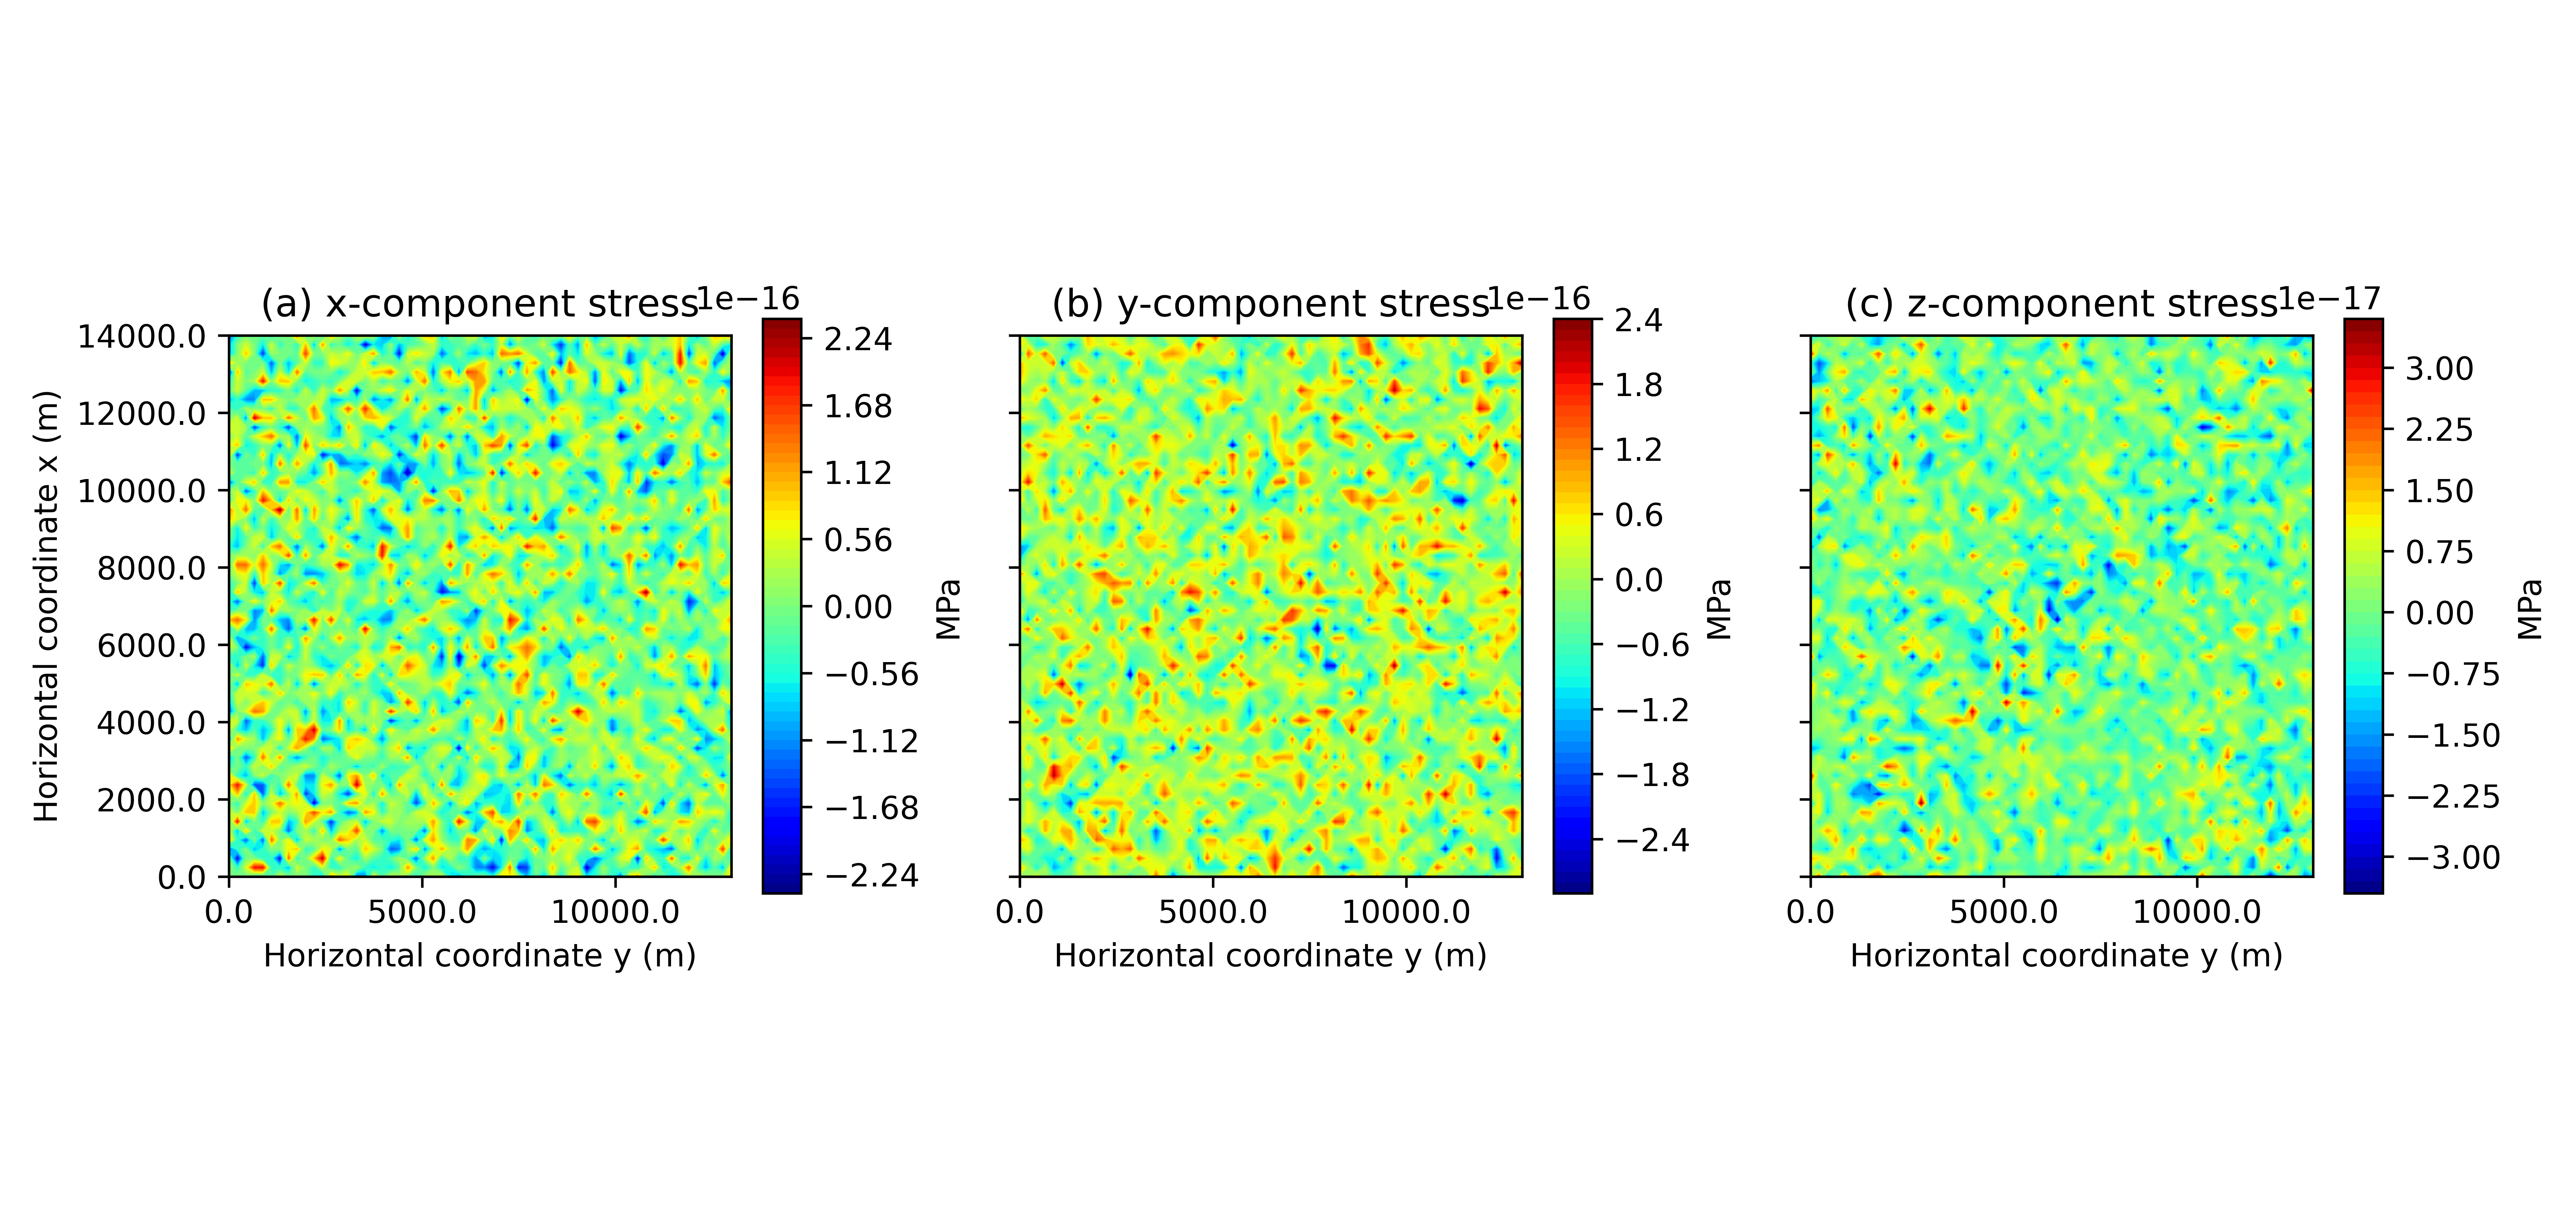
\includegraphics[width=12cm]{Fig/Figure_Null_stress_complex_reservoir.png}
\caption{Reservoir with arbitrary geometry and under arbitrary pressure changes: (a) $x-$, (b) $y-$, and (c) $z-$components of the stress at the free surface.}
\label{fig:Null_stress_complex_reservoir}
\end{figure}


%% Since the Copernicus LaTeX package includes the BibTeX style file copernicus.bst,
%% authors experienced with BibTeX only have to include the following two lines:
%%
%% \bibliographystyle{copernicus}
%% \bibliography{example.bib}
%%
%% URLs and DOIs can be entered in your BibTeX file as:
%%
%% URL = {http://www.xyz.org/~jones/idx_g.htm}
%% DOI = {10.5194/xyz}


%% LITERATURE CITATIONS
%%
%% command                        & example result
%% \citet{jones90}|               & Jones et al. (1990)
%% \citep{jones90}|               & (Jones et al., 1990)
%% \citep{jones90,jones93}|       & (Jones et al., 1990, 1993)
%% \citep[p.~32]{jones90}|        & (Jones et al., 1990, p.~32)
%% \citep[e.g.,][]{jones90}|      & (e.g., Jones et al., 1990)
%% \citep[e.g.,][p.~32]{jones90}| & (e.g., Jones et al., 1990, p.~32)
%% \citeauthor{jones90}|          & Jones et al.
%% \citeyear{jones90}|            & 1990


% Figures

%% FIGURES

%% When figures and tables are placed at the end of the MS (article in one-column style), please add \clearpage
%% between bibliography and first table and/or figure as well as between each table and/or figure.

% The figure files should be labelled correctly with Arabic numerals (e.g. fig01.jpg, fig02.png).


%% ONE-COLUMN FIGURES

%%f
%\begin{figure}[t]
%\includegraphics[width=8.3cm]{FILE NAME}
%\caption{TEXT}
%\end{figure}
%
%%% TWO-COLUMN FIGURES
%
%%f
%\begin{figure*}[t]
%\includegraphics[width=12cm]{FILE NAME}
%\caption{TEXT}
%\end{figure*}
%
%
%%% TABLES
%%%
%%% The different columns must be seperated with a & command and should
%%% end with \\ to identify the column brake.
%
%%% ONE-COLUMN TABLE
%
%%t
%\begin{table}[t]
%\caption{TEXT}
%\begin{tabular}{column = lcr}
%\tophline
%
%\middlehline
%
%\bottomhline
%\end{tabular}
%\belowtable{} % Table Footnotes
%\end{table}
%
%%% TWO-COLUMN TABLE
%
%%t
%\begin{table*}[t]
%\caption{TEXT}
%\begin{tabular}{column = lcr}
%\tophline
%
%\middlehline
%
%\bottomhline
%\end{tabular}
%\belowtable{} % Table Footnotes
%\end{table*}
%
%%% LANDSCAPE TABLE
%
%%t
%\begin{sidewaystable*}[t]
%\caption{TEXT}
%\begin{tabular}{column = lcr}
%\tophline
%
%\middlehline
%
%\bottomhline
%\end{tabular}
%\belowtable{} % Table Footnotes
%\end{sidewaystable*}
%
%
%%% MATHEMATICAL EXPRESSIONS
%
%%% All papers typeset by Copernicus Publications follow the math typesetting regulations
%%% given by the IUPAC Green Book (IUPAC: Quantities, Units and Symbols in Physical Chemistry,
%%% 2nd Edn., Blackwell Science, available at: http://old.iupac.org/publications/books/gbook/green_book_2ed.pdf, 1993).
%%%
%%% Physical quantities/variables are typeset in italic font (t for time, T for Temperature)
%%% Indices which are not defined are typeset in italic font (x, y, z, a, b, c)
%%% Items/objects which are defined are typeset in roman font (Car A, Car B)
%%% Descriptions/specifications which are defined by itself are typeset in roman font (abs, rel, ref, tot, net, ice)
%%% Abbreviations from 2 letters are typeset in roman font (RH, LAI)
%%% Vectors are identified in bold italic font using \vec{x}
%%% Matrices are identified in bold roman font
%%% Multiplication signs are typeset using the LaTeX commands \times (for vector products, grids, and exponential notations) or \cdot
%%% The character * should not be applied as mutliplication sign
%
%
%%% EQUATIONS
%
%%% Single-row equation
%
%\begin{equation}
%
%\end{equation}
%
%%% Multiline equation
%
%\begin{align}
%& 3 + 5 = 8\\
%& 3 + 5 = 8\\
%& 3 + 5 = 8
%\end{align}
%
%
%%% MATRICES
%
%\begin{matrix}
%x & y & z\\
%x & y & z\\
%x & y & z\\
%\end{matrix}
%
%
%%% ALGORITHM
%
%\begin{algorithm}
%\caption{...}
%\label{a1}
%\begin{algorithmic}
%...
%\end{algorithmic}
%\end{algorithm}
%
%
%%% CHEMICAL FORMULAS AND REACTIONS
%
%%% For formulas embedded in the text, please use \chem{}
%
%%% The reaction environment creates labels including the letter R, i.e. (R1), (R2), etc.
%
%\begin{reaction}
%%% \rightarrow should be used for normal (one-way) chemical reactions
%%% \rightleftharpoons should be used for equilibria
%%% \leftrightarrow should be used for resonance structures
%\end{reaction}
%
%
%%% PHYSICAL UNITS
%%%
%%% Please use \unit{} and apply the exponential notation


\end{document}
